% Synchronized to r29817
\include{fli4l}

\makeindex

\begin{document}

\newcommand{\titlename}{fli4l -- flexible internet router for linux}

\flhypersetup{pdftitle=\titlename}
\pdfbkmrk{-1}{\titlename}{title}
\title{\titlename\\ Version \version}

\author{Frank Meyer\\ \email{frank@fli4l.de} \and L'équipe fli4l\\ \email{team@fli4l.de}}

\maketitle
\pdfbkmrk{0}{\contentsname}{table}
\tableofcontents

% Last Update: $Id$
% Synchronized to r34514
\chapter{Documentation of the base package}

\section{Introduction}

fli4l is a Linux-based router, capable of handling ISDN, DSL, UMTS, and
ethernet connections, with little hardware requirements: an USB stick used for
booting, an Intel Pentium MMX processor, 64 MiB RAM as well as (at least) one
ethernet network adapter are completely sufficient. The necessary boot medium
can be created under Linux, Mac OS~X or MS~Windows. You don't need any specific Linux
knowledge, but it is definitely helpful. However, you should possess basic
knowledge about networking, TCP/IP, DNS, and routing. For developing your own
extensions exceeding the basic configuration, you will need a working Linux
system as well as Linux skills.

fli4l supports various boot media, among them USB sticks, hard disks, CDs, and
last but not least booting over the network. An USB stick is in many respects
ideal:  Today, almost every PC can boot from it, it is relatively cheap, it is
big enough, and installing fli4l onto it is relatively easy under both
MS~Windows and Linux. In contrast to a CD it is writable and thus additionally
able to hold non-volatile configuration data (as e.g. DHCP leases).

\begin{itemize}

\item General features

\begin{itemize}
\item Creation of boot media under \jump{sec:bootmedien_linux}{Linux},
      \jump{sec:bootmedien_linux}{Mac OS~X}, and
      \jump{sec:bootmedien_windows}{MS~Windows}
\item Configuration through flat ASCII/UTF-8 files
\item Support for IP masquerading and port forwarding
\item Least Cost Routing (LCR): automatic provider selection based on daytime
\item Displaying/Computing/Logging of connection times and costs
\item MS~Windows/Linux client imonc talking to imond and telmond
\item Upload of updated configuration files via MS~Windows client imonc or via
      SCP under Linux
\item Boot media use the VFAT file system as permanent storage
\item Packet filter: External access to blocked ports is logged
\item Uniform mapping of WAN interfaces to so-called circuits
\item Running ISDN and DSL/UMTS circuits in parallel is possible
\end{itemize}

\item Router basics

\begin{itemize}
\item Linux kernel 3.18 or 3.19
\item Packet filter and IP masquerading
\item Local DNS server in order to reduce the number of DNS queries to external
      DNS servers
\item Remotely accessible imond server daemon for monitoring and controlling
      Least Cost Routing
\item Remotely accessible telmond server daemon logging incoming phone calls
\end{itemize}

\item Ethernet support

\begin{itemize}
\item Up-to-date network device drivers: Support for more than 140 adapter types
\end{itemize}

\item DSL support

\begin{itemize}
\item Roaring Penguin PPPoE driver supporting Dial-on-Demand (can be switched
      off)
\item PPTP for DSL providers in Austria and the Netherlands
\end{itemize}

\item ISDN support

\begin{itemize}
\item Support for some 60 adapter types
\item Multiple possibilities for ISDN connectons: incoming/outgoing/callback,
      raw/point-to-point (ppp)
\item Channel bundling: automatic band width adaptation or manual activation of
      the second channel using MS~Windows/Linux client software
\end{itemize}

\item Optional software packages

\begin{itemize}
\item DNS server
\item DHCP server
\item SSH server
\item Simple online/offline display using a LED
\item Serial console
\item Minimalistic Web server for ISDN and DSL monitoring as well as
      for reconfiguring and/or updating the router
\item Ability to let external hosts access LAN hosts in a controlled manner
\item Support for PCMCIA cards (called PC cards nowadays)
\item Logging of system messages
\item Configuration of ISAPnP cards by the use of isapnp tools
\item Additional tools for debugging
\item Configuration of the serial port
\item Rescue system for remote administration over ISDN
\item Software for displaying configurable information on an LCD, e.g.
      transmission rates, CPU load etc.
\item PPP server/router over the serial port
\item ISDN modem emulator over the serial port
\item Print server
\item Time synchronization with external time servers
\item Execution of user-defined commands on incoming phone calls (e.g.
      to perform Internet dial-up)
\item Support for IP aliasing (multiple IP addresses per network interface)
\item VPN support
\item IPv6 support
\item WLAN support: fli4l can be an access point as well as a client
\item RRD tool for monitoring the fli4l
\item and much more\ldots
\end{itemize}

\item Hardware requirements

\begin{itemize}
\item Intel Pentium processor with MMX support
\item 64 MiB RAM, better 128 MiB
\item Ethernet network adapter
\item ISDN: supported ISDN adapter
\item an USB stick, an ATA hard disk or a CF card (which is accessed the same
      way as an ATA hard disk); alternatively, booting from a CD is also
      possible
\end{itemize}

\item Software requirements

The following tools are required on Linux systems:

\begin{itemize}
\item GCC and GNU make
\item syslinux
\item mtools (mcopy)
\end{itemize}

No additional tools are required on MS~Windows systems, all necessary tools are
provided by fli4l.

\end{itemize}

Last but not least, the client utility imonc exists for controlling the router
and for displaying the router's state. This tool is available for MS~Windows
(windows/imonc.exe) and also for Linux (unix/gtk-imonc).

And now \ldots \bigskip

Have fun with fli4l!\bigskip

Frank Meyer and the fli4l team

\email{team@fli4l.de}

% Last Update: $Id$
\chapter{Installation und Konfiguration}

\section{Entpacken der Archive}

Unter Linux:

\begin{verse}\texttt{tar xvfz fli4l-\version.tar.gz}\end{verse}

\noindent Funktioniert dies nicht, geht's auch so:

\begin{verse}\texttt{gzip -d < fli4l-\version.tar.gz | tar xvf -}\end{verse}

Wer die aktuelle Version in einem bereits existierenden
fli4l-Verzeichnis installiert, sollte anschließend
\texttt{mkfli4l.sh -c} aufrufen, also:

\begin{verse}
    \texttt{cd fli4l-\version}\\
    \texttt{sh mkfli4l.sh -c}
\end{verse}

Es wird jedoch empfohlen, ein neues Verzeichnis für eine neue Version
zu benutzen~-- die Konfiguration kann durch ein entsprechendes Werkzeug zum
Dateivergleich sehr einfach übernommen werden.

Unter MS~Windows kann das komprimierte Tar-Archiv zum Beispiel mit WinZip
extrahiert werden. Dabei ist jedoch zu beachten, dass die Dateien
\emph{mit} Unterverzeichnissen (Einstellung in WinZip überprüfen!)
ausgepackt werden. Außerdem ist in \emph{Optionen \pfeil
  Konfiguration} die so genannte "`Smart TAR CR conversion"'
abzuschalten. Ist diese eingeschaltet, werden einige wichtige
Dateien von WinZip falsch extrahiert.

Alternativ ist das OpenSource-Programm 7-Zip (\altlink{http://www.7-zip.org/})
sehr zu empfehlen, welches ebenso mächtig wie WinZip ist.

Es werden folgende Dateien im Unterverzeichnis
\texttt{fli4l-\version/} installiert:

\begin{itemize}
\item Dokumentation:
  \begin{itemize}
  \item doc/deutsch/* Deutsche Dokumentation
  \item doc/english/* Englische Dokumentation
  \item doc/french/*  Französische Dokumentation
  \end{itemize}

\item Konfiguration:
  \begin{itemize}
  \item config/*.txt Konfigurationsdateien, diese müssen bearbeitet
    werden
  \end{itemize}

\item Skripte/Prozeduren:
  \begin{itemize}
  \item mkfli4l.sh Boot-Medium oder Dateien erzeugen: Linux/Unix-Version
  \item mkfli4l.bat Boot-Medium erzeugen: Windows-Version
  \end{itemize}

\item Kernel/Boot-Dateien:
  \begin{itemize}
  \item img/kernel Linux-Kernel
  \item img/boot*.msg Bootscreen Texte
  \end{itemize}

\item Zusatzpakete:
  \begin{itemize}
  \item opt/*.txt Diese Dateien beschreiben, was bei welchen Einstellungen in
  das Archiv opt.img gelangt.
  \item opt/... Optionale Kernel-Module, Dateien und Programme
  \end{itemize}

\item Quellcode:
  \begin{itemize}
  \item src/* Quellcode/Werkzeuge für Linux, siehe src/README
  \end{itemize}

\item Programme:
  \begin{itemize}
  \item unix/mkfli4l* Erzeugen des Bootmediums: Unix/Linux-Version
  \item windows/* Erzeugen des Bootmediums: Windows-Version
  \item unix/imonc* imond-Client für Unix/Linux
  \item windows/imonc/* imond-Client für Windows
  \end{itemize}
\end{itemize}

\section{Konfiguration}
\subsection{Editieren der Konfigurationsdateien}

Zur Konfiguration von fli4l müssen lediglich die Dateien config/*.txt
angepasst werden. Um im Nachhinein die eigenen Konfiguration mit der
ausgelieferten vergleichen zu können oder um mehrere Konfigurationen
verwalten zu können, empfiehlt es sich, eine Kopie des
config-Verzeichnisses anzulegen und die Konfiguration in dieser Kopie
durchzuführen. Ein Vergleich der Konfigurationen ist dann durch
Verwendung eines geeigneten Werkzeugs (z.B. ``diff'' unter *nix) relativ
einfach möglich. Nehmen wir einmal an, die eigene config liegt in einem
Verzeichnis mit Namen ``meine\_config'' ebenfalls im fli4l-Verzeichnis
dann wäre der Aufruf wie folgt:
\begin{example}
\begin{verbatim}
    ~/src/fli4l> diff -u {config,meine_config}/build/rc.cfg | grep '^[+-]'
    --- config/build/rc.cfg    2014-02-18 15:34:39.085103706 +0100
    +++ meine_config/build/rc.cfg        2014-02-18 15:34:31.094317441 +0100
    -PASSWORD='/P6h4iOIN5Bbc'
    +PASSWORD='3P8F3KbjYgzUc'
    -NET_DRV_1='ne2k-pci'
    +NET_DRV_1='pcnet32'
    -START_IMOND='no'
    +START_IMOND='yes'
    -OPT_PPPOE='no'
    +OPT_PPPOE='yes'
    -PPPOE_USER='anonymer'
    -PPPOE_PASS='surfer'
    +PPPOE_USER='ich'
    +PPPOE_PASS='mein-passwd'
    -OPT_SSHD='no'
    +OPT_SSHD='yes'
\end{verbatim}
\end{example}

Man sieht hier auch sehr schön, dass ein einfacher DSL-Router mit
wenigen Handgriffen konfiguriert ist, auch wenn einen die
Konfigurationsdateien auf den ersten Blick mit ihrer Fülle von
Einstellungsmöglichkeiten erschlagen.

\subsection{Konfiguration über eine spezielle Konfigurationsdatei}

Da sich die Konfiguration durch das Modul-Konzept auf verschiedene
Dateien verteilt, und das Bearbeiten dadurch unter Umständen etwas
mühsam wird, kann man die Konfiguration auch in einer einzelnen Datei
namens \emph{$<$config~verzeichnis$>$/\_fli4l.txt} ablegen, deren Inhalt
dann zusätzlich zu den normalen Konfigurationsdateien eingelesen wird
und deren Inhalt dominiert. Um beim obigen Beispiel zu bleiben: Um
einen einfachen DSL-Router zu konfigurieren, könnten wir einfach
folgendes in diese Datei schreiben:

\begin{example}
\begin{verbatim}
    PASSWORD='3P8F3KbjYgzUc'
    NET_DRV_N='1'
    NET_DRV_1='pcnet32'
    START_IMOND='yes'
    OPT_PPPOE='yes'
    PPPOE_USER='ich'
    PPPOE_PASS='mein-passwd'
    OPT_SSHD='yes'
\end{verbatim}
\end{example}

Man sollte vermeiden, beide Konfigurationsvarianten zu mischen.

\subsection{Variablen}

  Sie werden merken, dass einige Variablen auskommentiert sind. Wenn das der 
  Fall ist, erhält sie eine sinnvolle Standard-Belegung. Diese Standard-Belegung 
  ist für jede Variable dokumentiert. Wünschen Sie einen anderen Wert für diese 
  Variable, sollten Sie das Kommentarzeichen am Anfang der Variablendefinition ('\#') 
  entfernen und den entsprechenden Wert zwischen den Hochkommata einfügen.

\marklabel{VARIANTEN}{\section{Installationsvarianten}}

In den vorhergehenden Versionen von fli4l wurde lediglich das Booten
von einer Diskette unterstützt. Dies ist aus oben genannten Gründen nun
nicht mehr möglich, aber die Alternative mittels eines USB-Sticks ist 
gegeben.

Es sind auch eine Vielzahl anderer Bootmedien (CD, HD, Netzwerk,
Compact-Flash, DoC, \ldots) möglich und fli4l kann auch auf diversen
Medien installiert (HD, Compact-Flash, DoC) werden. Dazu kann fli4l auf
drei verschiedenen Wegen gebootet werden:

\begin{description}
\item [Single Image] Der Bootloader lädt den Linux-Kern und dann fli4l
als ein einziges Image --- danach kann fli4l ohne weiteren Zugriff auf
andere Medien booten. Beispiele dafür sind die Boottypen \emph{integrated}, 
\emph{attached}, \emph{netboot} und \emph{cd}.
\item [Split Image] Der Bootloader lädt den Linux-Kern und dann ein
rudimentäres fli4l-Image, dass die Bootmedien einbindet und die
Konfiguration und restlichen Dateien aus einem dort liegenden Archiv
holt. Beispiele dafür sind diese Boottypen: \emph{hd (Typ A)}, \emph{ls120},
\emph{attached} und \emph{cd-emul}.
\item [Installation auf einem Medium] Der Bootloader lädt den
Linux-Kern und dann ein rudimentäres fli4l-Image, das eine bereits
vorhandene fli4l-Installation in sein Dateisystem einbindet und damit
keine weiteren Archive auspacken muss. Eine HD-Installation vom Typ B
ist ein Beispiel dafür.
\end{description}

Man sollte jedoch zunächst erst einmal fli4l in einer minimalen Version 
installieren und damit Erfahrungen sammeln. Möchte man später fli4l 
zusätzlich als Anrufbeantworter und als HTTP-Proxy einsetzen, so hat 
man vorher schon mal Erfahrungen mit einem grundsätzlich laufenden Router.

Für die Installation ergeben sich daraus die folgenden fünf Varianten:

\begin{description}
\item[USB-Stick] Router auf einem USB-Stick
\item[CD-router] Router auf einer CD
\item[Netzwerk] Netzwerkboot
\item[HD-Installation Typ A] Router auf Festplatte, CF, DoC~-- nur eine FAT-Partition
\item[HD-Installation Typ B] Router auf Festplatte, CF, DoC~-- je eine FAT- und ext3-Partition
\end{description}

\marklabel{INSTALLTYP0}{\subsection{Router auf einem USB-Stick}}

USB-Sticks werden von Linux als Festplatten angesprochen, daher gelten hier
die Ausführungen zur Festplatteninstallation entsprechend. Bitte beachten Sie,
dass mittels des \var{OPT\_\-USB} die entspechenden Treiber geladen werden
müssen, damit der Stick mittels \var{OPT\_\-HDINSTALL} eingebunden werden kann.

\marklabel{INSTALLTYP0}{\subsection{Router auf einer CD oder Netzwerkboot}}

Alle benötigten Dateien liegen auf dem Bootmedium und werden beim
Booten in eine dynamische RAM-Disk entpackt.  In einer
Minimalkonfiguration ist damit ein Betrieb des Routers mit nur 64 MiB
RAM möglich. Die maximale Konfiguration wird nur durch die Kapazität
des Bootmediums und des Hauptspeichers limitiert.

\marklabel{INSTALLTYPA}{\subsection{Typ A: Router auf Festplatte~-- nur eine FAT-Partition}}

Dies entspricht der CD-version, nur dass die Dateien hierbei auf
einer Festplatte liegen, wobei der Begriff \glqq{}Festplatte\grqq{} hier auch
Compact-Flash-Medien ab 8 MiB und andere Geräte, welche Linux als
Festplatte ansprechen kann, mit einschließt. Seit fli4l 2.1.4 können
auch DiskOnChip Flash-Speicher von M-Sys oder SCSI-Festplatten benutzt
werden.

Die Beschränkung des Archivs opt.img durch die
Diskettenkapazität wird aufgehoben, aber alle diese Dateien müssen in
einer RAM-Disk mit der entsprechenden Größe beim Boot installiert werden.
Dies erhöht den RAM-Bedarf beim Einsatz vieler Pakete.

Für ein Update der Softwarepakete (d.h. des Archivs opt.img und der
rc.cfg über das Netzwerk) muss die FAT-Partition genügend Platz für den
Kernel, das RootFS und die DOPPELTE Größe des opt.img haben!
Falls auch die Notfall-Option genutzt werden soll, erhöht sich der
Platzbedarf noch einmal um die Größe des opt.img.

\marklabel{INSTALLTYPB}{\subsection{Typ B: Router auf Festplatte~-- je eine FAT- und ext3-Partition}}

Im Gegensatz zum Typ A werden hier nicht alle Dateien in die Ramdisk
gepackt, sondern bei dem erstmaligen Start nach der Installation oder
nach einem Update aus dem Archiv opt.img direkt auf eine
ext3-Partition kopiert und im späteren Betrieb von dort geladen. Bei
dieser Version ist der Speicherbedarf für die RAM-Disk am geringsten
und damit meist auch ein Betrieb mit sehr wenig RAM möglich.

Weitere Informationen zur Installation auf Festplatten finden Sie in
der Dokumentation des Pakets HD (separat herunterzuladen)-
beginnend bei der Beschreibung der Variablen \var{OPT\_\-HDINSTALL}.

% Last Update: $Id$
\chapter{Basiskonfiguration}

Ab Version 2.0 ist die fli4l-Distribution modular aufgebaut und in
mehrere Pakete aufgeteilt, die extra heruntergeladen werden müssen. Im
Paket \texttt{fli4l-\version.tar.gz} ist lediglich die
Basis-Software für einen Ethernet-Router enthalten. Für DSL, ISDN und
weitere Software müssen die Pakete separat heruntergeladen werden und
ausgehend vom Verzeichnis \texttt{fli4l-\version/} (!) installiert
werden. Durch die Auswahlmöglichkeit des Betriebssystemkerns von fli4l
sind diese in die Kernel Pakete ausgelagert worden. Somit ist als Minimum
Basis und ein Kernel Paket erforderlich.
In Tabelle \ref{tab:zusatzpakete} finden Sie einen
Überblick über die Zusatzpakete.

\begin{table}[ht!]
 \caption{Übersicht über die (Zusatz-)Pakete}\marklabel{tab:zusatzpakete}{}
  \begin{center}
    \begin{tabular}{ll}
      \textbf{Download-Archiv}        &    \textbf{Paket} \\
      \hline
      \texttt{fli4l-\version}         &    BASIS, erforderlich!\\
      \verb*zkernel_4_19z             &    Linux-Kernel, erforderlich!\\
      \texttt{fli4l-\version-doc}     &    Komplette Dokumentation\\
      \verb*zadvanced_networkingz     &    Erweiterte Netzwerkkonfiguration\\
      \verb*zcertz                    &    Zertifikatsverwaltung\\
      \verb*zchronyz                  &    Time-Server/Client\\
      \verb*zdhcp_clientz             &    Verschiedene DHCP-Clients\\
      \verb*zdns_dhcpz                &    DNS- und DHCP-Server\\
      \verb*zdslmodemz                &    Unterstützung für interne DSL-Modems (z.B. AVM Fritz!DSL)\\
      \verb*zdyndnsz                  &    Unterstützung von DYNDNS-Diensten\\
      \verb*zeasycronz                &    Zeitplandienst\\
      \verb*zhdz                      &    Installation auf Festplatte\\
      \verb*zhttpdz                   &    Mini-Webserver für Status-Ausgaben\\
      \verb*zhwsuppz                  &    Unterstützung von Hardware\\
      \verb*zimonc_windowsz           &    Der Windows-Imonc\\
      \verb*zimonc_unixz              &    Der GTK-Unix-Imonc\\
      \verb*zipv6z                    &    Internet Protokoll Version 6\\
      \verb*zisdnz                    &    ISDN-Router\\
      \verb*zopenvpnz                 &    OpenVPN-Unterstützung\\
      \verb*zpcmciaz                  &    Unterstützung von PCMCIA-Karten\\
      \verb*zpppz                     &    PPP-Basispaket\\
      \verb*zpppoez                   &    DSL-Router (PPPoE)\\
      \verb*zproxyz                   &    Proxy-Server\\
      \verb*zqosz                     &    Quality of Service\\
      \verb*zsshdz                    &    SSH-Server\\
      \verb*ztoolsz                   &    Diverse Linux-Werkzeuge\\
      \verb*zumtsz                    &    Anbindung mittels UMTS an das Internet\\
      \verb*zusbz                     &    Unterstützung der USB-Schnittstelle\\
      \verb*zvpnz                     &    VPN (PPTP)\\
      \verb*zwlanz                    &    Unterstützung von WLAN-Karten
    \end{tabular}
  \end{center}
\end{table}

Die zur Konfiguration des fli4l-Routers verwendeten Dateien
befinden sich im Verzeichnis \texttt{config/} und werden hier im Folgenden
beschrieben.

Diese Dateien können mit einem \emph{einfachen} Text-Editor oder auch
mit einem speziell an fli4l angepassten Editor verändert werden. Diverse
Editoren sind unter

\par

\altlink{http://www.fli4l.de/download/zusatzpakete/addons/} zu finden.

Sind spezielle Anpassungen/Erweiterungen erforderlich, die über die
unten aufgeführten Einstellungsmöglichkeiten hinausgehen, benötigt man
ein lauffähiges Linux-System, um Anpassungen im RootFS vorzunehmen. In
diesem Fall hilft \verb+src/README+ weiter.

\newpage

% Do not remove the next line
% Synchronized to r29818

\marklabel{beispielbase}{\section{Exemple de fichier}}\index{Exemple de fichier (base.txt)}\index{base.txt}

L'exemple fichier de \verb+base.txt+ qui est dans le répertoire \verb+config/+ a
le contenu suivant:~:

\begin{example}
\verbatimfile{\basedir/config/base.txt}
\end{example}

\medskip

Ce fichier est enregistré sous le format DOS. Cela signifie, qu'à l'extrémité
de chaque ligne, il y a un retour chariot (CR). J'ai décidé d'utiliser ce format
car la plupart des éditeurs Unix ne rencontreront aucun problème avec. Le
bloc-notes de Windows, ne peut pas manipuler ces fichiers sans CRs~!

Si vous avez, des problèmes avec votre éditeur Unix/Linux favori, vous pouvez
employer la commande suivante avant d'éditer le fichier au format Unix~:

\begin{example}
\begin{verbatim}
        sh unix/dtou config/base.txt
\end{verbatim}
\end{example}

Lors de la création du support de boot, il n'y a aucune importance si le fichier
contient ou pas des CRs en fin de lignes. Lorsque le fichier sera écrit sur le
support de boot ou sur le disque dur, tout les CRs et tous les commentaires,
seront complètement ignorés.

Maintenant nous pouvons commencer \ldots
% Synchronized to r51346

\section{General settings}

\begin{description}

  \config{HOSTNAME}{HOSTNAME}{HOSTNAME}

  Default Setting: \var{HOSTNAME='fli4l'}
  
  At the very beginning you should choose a name for your fli4l router.


  \config{PASSWORD}{PASSWORD}{PASSWORD}

  Default Setting: \var{PASSWORD='fli4l'}
  
  This password is needed for logging on to the router---regardless whether
  you use a keyboard attached to the router or a remote SSH console
  (for the latter you will need the sshd package). The minimum password
  length is 1, the maximum 126 characters.

  \config{BOOT\_TYPE}{BOOT\_TYPE}{BOOTTYPE}

  Default setting: \var{BOOT\_TYPE='hd'}

  \var{BOOT\_TYPE} determines the boot medium in the broadest sense and
  affects the drivers (kernel modules) and start scripts being included in
  the RootFS. A short description of the boot process for
  better understanding:

  \begin{itemize}
  \item The BIOS of the computer loads and starts the boot loader on the boot
        medium.
  \item The boot loader (typically syslinux) extracts, loads, and starts the
        kernel.
  \item The kernel extracts the RootFS (= the basic file system containing
        tools and scripts needed for booting), mounts the RootFS and begins to
        execute the start scripts.
  \item Depending on \var{BOOT\_TYPE}, the start scripts loads the kernel modules
        for the boot medium, mounts the boot partition, and extracts the OPT
        archive (\texttt{opt.img}) containing additional programs.
  \item Subsequently, fli4l starts to configure the individual services.
  \end{itemize}

  The following values are valid for \var{BOOT\_TYPE} at the moment:

  \begin{description}
  \item[ls120] Choose this to boot from LS120/240 and ZIP disks.
  \item[hd] Choose this to boot from a hard disk. You will find more information in the
    \jump{sec:hdinstall}{Documentation} of the HD package.
  \item[cd] Choose this to boot from CD-ROM. With this setting, the ISO image fli4l.iso will be created which
    you have to burn onto CD with your favourite CD burning application.
    Please pay attention to choosing the right driver for your CD drive.
  \item[integrated] Choose this if you do not plan to use a conventional boot
    medium but e.g. want to boot over a network. This setting integrates the
    OPT archive into the RootFS so the kernel can extract everything at once
    and does not need not mount a boot medium.\\
    \textbf{Note: } You cannot perform a remote update of your fli4l router in
    this case.
  \item[attached]
    This setting is similar to \textbf{integrated} but it does not integrate the
    contents of the OPT archive into the RootFS; rather, the OPT archive is
    put ``as is'' into the \texttt{/boot} directory. From there it will be
    extracted during the boot process.\\
    Apart from that, the caveats described for \texttt{integrated} apply to this
    boot type as well.
  \item[netboot]
    This setting corresponds to \textbf{integrated}. However, the script
    \texttt{mknetboot.sh} is additionally run to create an image for booting
    over the local network. Please read the wiki
    \altlink{https://ssl.nettworks.org/wiki/display/f/fli4l+und+Netzboot}
    for further information.\\
  \item[pxeboot]
    Two images are generated, kernel and rootfs.img. These are the two files to be loaded
    by the PXE bootloader. During execution the local tftp directory may be specified and
    in addition a subdirectory in the tftp directory (--pxesubdir).
    Refer to the Wiki here as well:
    \altlink{https://ssl.nettworks.org/wiki/display/f/fli4l+und+Netzboot}.
  \end{description}

   \textbf{Note:} How to configure fli4l as a boot-server (pxe/tftp) you 
    can find in the documentation of opt dns\_dhcp!
  
  \config{LIBATA\_DMA}{LIBATA\_DMA}{LIBATADMA}
  
  Default Setting: \var{LIBATA\_DMA='disabled'}

  This options selects if DMA is used for libata based Devices. It is needed 
  for example for incompletely wired IDE to CompactFlash Adapters. Select
  'enabled' to use DMA.

  \config{MOUNT\_BOOT}{MOUNT\_BOOT}{MOUNTBOOT}
  
  Default Setting: \var{MOUNT\_\-BOOT='rw'}
  
  {This variable specifies how to mount the boot medium. There are three
  possibilities:

    \begin{description}
    \item[rw]~-- Read/Write~-- Writing and reading is possible
    \item[ro]~-- Read-Only~-- Only reading is possible
    \item[no]~-- None~-- Medium will be unmounted after booting and can then
      be removed if desired
    \end{description}

    Some configurations require mounting the boot medium read/write, e.g. if
    you want to run a DHCP server or if you want the imond log file to be
    stored on the boot medium.}

  \config{BOOTMENU\_TIME}{BOOTMENU\_TIME}{BOOTMENUTIME}

  Default setting: \var{BOOTMENU\_TIME='20'}

  {This variable controls how LONG the syslinux boot loader should wait
   until the default installation is booted automatically.

    The \var{OPT\_RECOVER} variable of the HD package allows you to activate
    a function which enables you to create a recovery installation from a
    working installation. This recovery installation can be activated in the
    boot menu by choosing the recovery version.

    If this variable contains the value '0', the syslinux boot loader will
    wait indefinitely until the user chooses either the default or the
    recovery installation!}

  \config{TIME\_INFO}{TIME\_INFO}{TIMEINFO}
  
  Default Setting: \var{TIME\_INFO='MEZ-1MESZ,M3.5.0,M10.5.0/3'}

  Normally, Unix operating systems use the UTC (Coordinated Universal Time)
  for clocks running under their control, and so does fli4l. The UTC is
  consistent around the world and has to be converted to local time before
  use. By using \var{TIME\_\-INFO}, you provide the necessary information for
  fli4l about your time zone, its difference to UTC, and about daylight
  saving time. Your local hardware clock must be set to UTC (corresponds to
  London Standard Time) in order to make these settinge effective.
  Alternatively, you may use the chrony Package which allows fli4l to
  synchronize its clock with an external time server (time servers always
  provide the current time in UTC).

  The meaning of the possible settings \var{TIME\_\-INFO} are as
  follows:
\begin{example}
\begin{verbatim}
        TIME_INFO='MEZ-1MESZ,M3.5.0,M10.5.0/3'
\end{verbatim}
\end{example}
  \begin{itemize}
  \item \emph{MEZ-1:} ``MEZ'' is the German abbreviation for ``Central European
  Time'' (you could also use ``CET'' here). The ``-1'' means that \emph{MEZ-1=UTC},
  i.e. the MEZ is one hour ahead of UTC.
  \item \emph{MESZ:} ``MESZ'' is the abbreviation for ``Central European Summer
  Time'' and means that fli4l has to handle daylight saving changes.
  Because no further information (``+x'' or ``-x'') is given, the clock is
  adjusted forward one hour when reaching the daylight saving time.
  \item \emph{M3.5.0,M10.5.0/3:} This means that the change to the daylight
  saving time occurs on the last Sunday in March at two o'clock and that the
  change to standard time occurs on the last Sunday in October at three
  o'clock.
  \end{itemize}

  Normally you do not have to touch these settings, unless your fli4l router
  resides in another time zone. In this case you have to adjust these settings 
  accordingly. In order to do this properly, it is helpful to take a look at the
  specification of the TZ environment variable which can be found at the
  following URL:

  \altlink{http://pubs.opengroup.org/onlinepubs/009695399/basedefs/xbd_chap08.html}

  \config{RTC\_SYNC}{RTC\_SYNC}{RTCSYNC}{
  Default Setting: \var{RTC\_SYNC='hwclock'}

  Many computers have a battery-backed hardware clock, which is also supplied with power
  while the system is powered off. This enables the system time to be running continuously
  even then in order to have a valid system time at the next system startup.
  At this point it is important to differentiate between the \emph{system time}
  and the \emph{hardware time}:
 
  \begin{itemize}
  \item \emph{Hardware time} is the time stored in the hardware clock
  and kept up to date by the device. It is usually read at system startup and
  becomes system time then.

  \item \emph{System time} is the time used by the linux system, i.e. if executing
  the command \texttt{date -u}. It is kept up to date by the Linux kernel, for example
  using hardware interrupts on a regular basis (timer interrupts) and always
  indicates a time in coordinated Universal Time (UTC). Hence it is not affected
  by any time zone settings.
 
  \item \emph{localized system time} is only the conversion of system time to
  another time zone. On the fli4l router it is configured by the environment
  variable \texttt{TZ} (see \jump{TIMEINFO}{\var{TIME\_INFO}}). This is not of
  any intertest for the further explanations below.
  \end{itemize}
  
  With the help of this variable you may configure how fli4l handles the adjustment
  between hardware time and system time, meaning if and how often hardware time
  should be set to the system time. Such an adjustment is necessary because even
  the best hardware clock is not 100 percent accurate and tends to systematic
  drifting, in the long run it will be a bit too slow or too fast.
  
  There are basically two ways of synchronization:
  
  \begin{itemize}
  \item ``kernel'' mode: An NTP client is used to get the real time from outside
  (usually via the Internet or an external (radio) clock) and keep the system 
  time of the fli4l router up to date. The Linux kernel takes care of updating
  the hardware time, so no further synchronization is needed. The update by the
  Linux kernel is a little less accurate than updating by \texttt{hwclock}
  (see `` hwclock '' mode below), however, the quality of the update is
  less important because errors are compensated by the NTP client.
  
  This mode must also be used if no hardware clock at all exists. The Linux kernel
  will not keep hardware time up-to-date in this case simply because there is none. In
  order to have a realistic system time at all, the use of a NTP client should
  be mandatory.
   
  \item Modus ``hwclock'': At shutdown of the system (when running the stop-script\\
  \texttt{/etc/rc0.d/rc950.hwclock}) and in regular intervals (every 24 hours) a
  synchronization using the \texttt{hwclock} program will take place. Not only the
  hardware time is set, but \texttt{hwclock} also measures to what extent the system
  time differs from the hardware time. When starting the system the system time is 
  not taken directly from the hardware time, the time drift is also taken into account
  in order to minimize drifting of the system time. The drift is stored in the file
  \texttt{/etc/adjtime}. If a writable persistent medium is available, the drift is
  stored in \texttt{/var/lib/persistent/base/adjtime}, in this case \texttt{/etc/adjtime}
  is a symbolic link pointing there.
  
  This mode is incompatible with updating the system time by the help of an NTP client.
  That's because an NTP client automatically enables updating the hardware clock by
  the Linux kernel. It is however, of little sense or problematic that both \texttt{hwclock}
  and the Linux kernel at the same time try to keep the hardware time up to date.
  \end{itemize}
  
  It should be noted that if a hardware clock is available, the time stored there
  is \emph{always} interpreted as coordinated world time (UTC). The time zone
  defined by the variable \var{TIME\_INFO} does not affect the time stored
  in the hardware clock. Saving a localized non-UTC time in the hardware clock
  is \emph{not} supported by fli4l.
  
  Loading the system time from the hardware time is done only once at system startup.
  The Linux kernel then reads the time stored in the hardware clock and sets system
  right at the beginning f the boot process. In ``hwclock'' mode the time will be
  set again later when running the boot script \texttt{/etc/rc.d/rc100.hwclock},
  this time taking into account the system's time drift.}

  \config{KERNEL\_VERSION}{KERNEL\_VERSION}{KERNELVERSION}

  Chooses the version of the kernel to be used. According to the contents of
  this variable, the kernel and the kernel modules are selected from
  \emph{img/kernel-$<$kernel version$>$.$<$compression extension$>$} and
  \emph{opt/lib/modules/$<$kernel version$>$}, respectively.

  \config{KERNEL\_BOOT\_OPTION}{KERNEL\_BOOT\_OPTION}{KERNELBOOTOPTION}
  
  Default Setting: \var{KERNEL\_BOOT\_OPTION=''}

  The contents of this variable is appended to the kernel's command line
  defined in syslinux.cfg. Some systems require 'reboot=bios' for proper 
  rebooting, i.e. WRAP systems.

  \config{COMP\_TYPE\_ROOTFS}{COMP\_TYPE\_ROOTFS}{COMPTYPEROOTFS}

  Default setting: \var{COMP\_TYPE\_ROOTFS='xz'}

  This variable selects the compression method to be used for the RootFS
  archive. Possible values are 'xz', 'lzma', and 'bzip2'.

  \config{COMP\_TYPE\_OPT}{COMP\_TYPE\_OPT}{COMPTYPEOPT}

  Default setting: \var{COMP\_TYPE\_OPT='xz'}

  This variable selects the compression method to be used for the OPT archive.
  Possible values are 'xz', 'lzma', and 'bzip2'.

  \config{POWERMANAGEMENT}{POWERMANAGEMENT}{POWERMANAGEMENT} 
  
  Default Setting: \var{POWERMANAGEMENT='acpi'}
  
  {
  The kernel supports different flavours of power management: the somewhat aged
  APM and the newer ACPI. This variable lets you choose which flavour is to be
  used. Possible values are 'none' (no power management), 'acpi', and the two
  APM variants 'apm' and 'apm\_rm'. The latter uses a special processor mode
  before switching the router off.}

  \config{FLI4L\_UUID}{FLI4L\_UUID}{FLI4LUUID}
  
  Default Setting: \var{FLI4L\_UUID=''}

    {This variable contains an universally unique identifier (UUID) which is used
    to point to a place where persistent data can be stored, e.g. on a USB
    stick. The UUID can be generated on any Linux system (e.g. on the fli4l
    router) by executing \verb*?'cat /proc/sys/kernel/random/uuid'?.
    Each execution of this command above produces a new UUID which you can
    use in \var{FLI4L\_UUID} variable. If you create a directory on
    a persistent medium by the name of this UUID, this directory will
    be used to store configuration changes as well as persistent run-time data
    (e.g. DHCP leases). However, the corresponding packages has to support
    this persistence mechanism (see the documentation to check this).
    Typically, use 'auto' for the according storage location, instead 
    of a hard-coded path.

    If fli4l already stored data using this mechanism before configuring an
    UUID and creating the directory, this data can be found under
    /boot/persistent. In this case, you will have to manually move the data to
    the new location. We advice that you generate and configure
    the UUID at the very beginning, avoiding the migration later on.

    Additionally, please note that \var{MOUNT\_BOOT}='rw' is needed
    if the storage directory is located on the /boot partition.

    We suggest using the /data partition (with the UUID-named directory being a
    top-level directory there) or an USB stick for the storage location of
    persistent configuration and run-time data. The file systems allowed are
    VFAT or, if you use OPT\_HD all read-writable filesystems supported there.}

  \config{IP\_CONNTRACK\_MAX}{IP\_CONNTRACK\_MAX}{IPCONNTRACKMAX}
  
  Default Setting: \var{IP\_CONNTRACK\_MAX=''}

  This variable enables you to change the maximum number of simultaneously existing
  connections. Normally, a sensible value for this setting is computed
  automatically, based on the amount of your router's physical RAM. Table
  \ref{tab:connectiontracking} shows the defaults used.

    \begin{table}[ht!]
        \centering
        \caption{Automtically generated maximum number of simultaneous connections}\marklabel{tab:connectiontracking}{}
        \begin{tabular}{p{6cm}p{6cm}}
            RAM in MiB               &    simultaneous connections \\\hline
            16                       &    1024 \\
            24                       &    1280 \\
            32                       &    2048 \\
            64                       &    4096 \\
            128                      &    8192 \\
        \end{tabular}
    \end{table}

   If you use file sharing programs behind or on the router and your router
   has only little RAM, you will hit the maximum number of simultaneous
   connections fastly. This will prevent further connections to be
   established.\\
   This causes error messages as

\begin{example}
\begin{verbatim}
        ip_conntrack: table full, dropping packet
\end{verbatim}
\end{example}

or

\begin{example}
\begin{verbatim}
        ip_conntrack: Maximum limit of XXX entries exceeded
\end{verbatim}
\end{example}

    The variable \var{IP\_\-CONNTRACK\_\-MAX} changes the maximum
    number of simultaneously existing connections to a fixed value.
    Each possible connection consumes 350 bytes of RAM, which
    cannot be used for other things. If you e.g. choose the value '10000',
    you reserve about 3,34 MB RAM that are lost for any other usage
    (kernel, RAM disks, programs).

    If your router has 32 MiB RAM, it should not be much of a problem to
    reserve 2 or 3 MiB for the ip\_conntrack table. If only 16 MiB RAM or less
    are available you should be more conservative to prevent your router from
    running out of RAM.

    The setting currently being used can be display on the console by executing

\begin{example}
\begin{verbatim}
        cat /proc/sys/net/ipv4/ip_conntrack_max
\end{verbatim}
\end{example}

    and can be set on-the-fly by executing

\begin{example}
\begin{verbatim}
        echo "XXX" > /proc/sys/net/ipv4/ip_conntrack_max
\end{verbatim}
\end{example}

    where XXX denotes the number of entries.
    The entries of the \var{IP\_CONNTRACK} table can be displayed on the
    console by executing

\begin{example}
\begin{verbatim}
        cat /proc/net/ip_conntrack
\end{verbatim}
\end{example}

    and can be counted by executing

\begin{example}
\begin{verbatim}
        cat /proc/net/ip_conntrack | grep -c use
\end{verbatim}
\end{example}

  \config{LOCALE}{LOCALE}{LOCALE}

  Default setting: \var{LOCALE}='de'

  Meanwhile, some fli4l components support multiple languages, for example
  the console menu and the Web GUI. This variable lets you choose your
  preferred language. In addition, some components support a private setting
  to override this global setting if necessary. English is used as a fallback
  if the language chosen is not supported for some component.

  \var{KEYBOARD\_LOCALE}='auto' tries to find a keyboard layout that is
  compatible with the \var{LOCALE} setting.

  By now, the following values are possible: de, en, fr.

\end{description}

% Synchronized to r54214

\marklabel{CONSOLESETTINGS}{\section{Console settings}}

fli4l can be operated on different hardware platforms. On many of these
platforms it is possible to have a keyboard and a monitor connected to 
interact with fli4l; this inpu/output combination is generally \emph{console}.

fli4l can also be used completely without keyboard and graphics card. 
In order to use the router as well without network access to it and 
to see all kernel boot messages, it is possible to use a console on a 
serial port catching inputs from the serial interface or sending output there. 
This requires the variables
\jump{SERCONSOLE}{\var{SER\_CONSOLE}},
\jump{SERCONSOLEIF}{\var{SER\_CONSOLE\_IF}} und
\jump{SERCONSOLERATE}{\var{SER\_CONSOLE\_RATE}} to be set resp. adapted.

It is also possible to use a console on both keyboard and monitor as well as 
via the serial port.

In general, fli4l provides the option to login and thus a \emph{Shell} on
\emph{any} console giving you the ability to login as the user ``fli4l'' 
with the password defined in \jump{PASSWORD}{\var{PASSWORD}}.

\begin{description}
  \config{CONSOLE\_BLANK\_TIME}{CONSOLE\_BLANK\_TIME}{CONSOLEBLANKTIME}
  
  Defaut Setting: \var{CONSOLE\_BLANK\_TIME=''}
  
  Typically, the Linux kernel activates the console's screen saver after some
  time without console input activity. The variable \var{CONSOLE\_BLANK\_TIME}
  allows you to configure the timeout to be used or to disable the screen saver
  completely (\var{CONSOLE\_BLANK\_TIME}='0').

  \config{BEEP}{BEEP}{BEEP}
  
  Defaut Setting: \var{BEEP='yes'}
  
  {Causes a beep at the end of the boot or shutdown process.

    If you enter `yes' here, there will be a beep at the end of the boot or
    shutdown process. If you suffer from an extreme shortage of space on your
    boot media or if you don't like your router to beep, use `no' instead.}

  \config{SER\_CONSOLE}{SER\_CONSOLE}{SERCONSOLE}
  
    Default Setting: \var{SER\_CONSOLE='no}'

    This variable enables or disables a console on a serial port. The serial 
    console can be operated in three modes:

      \begin{tabular}[h!]{|l|p{9cm}|}
        \hline
        \var{SER\_CONSOLE} & console input/outpute \\
        \hline
        no & Input and output (only) via keyboard and monitor (tty0) \\
        yes & Input and output (only) via serial interface (ttyS0) \\
        primary & Input and output via serial console as well as via 
        keyboard and monitor, output of kernel messages tty0 \\
        secondary & Input and output via serial console as well 
        as via keyboard and monitor, output of kernel messages ttyS0 \\
        \hline
      \end{tabular}
    
    Changing the value of \var{SER\_CONSOLE} affects the router only if you
    also update your boot media or if you perform a remote update of the
    syslinux.cfg file.

    \wichtig{When turning off the serial console, be sure to keep an alternate
    access to the router (SSH or directly from the keyboard and monitor)!}

    You will find further information in the appendix under
    \jump{SERIALCONSOLE}{Serial console}.


  \config{SER\_CONSOLE\_IF}{SER\_CONSOLE\_IF}{SERCONSOLEIF}
  
    Default Setting: \var{SER\_CONSOLE\_IF='0'}
  
  {
    Number of the serial interface for the serial console.

    Enter the number of the interface to which the serial console is connected.
    0 corresponds to ttyS0 under Linux or COM1 under Microsoft Windows.
  }

  \config{SER\_CONSOLE\_RATE}{SER\_CONSOLE\_RATE}{SERCONSOLERATE}
  
  Default Setting: \var{SER\_CONSOLE\_RATE='9600'}
  
  {Transmission rate of the serial port for console output.

    This variable contains the Baud rate to use for transmitting data over
    the serial port. Reasonable values are: 4800, 9600, 19200, 38400, 57600,
    115200.}

\end{description}

% Last Update: $Id$
\section{Hilfen zum Einkreisen von Problemen und Fehlern}

fli4l loggt die gesamten Ausgaben des Bootvorganges in einer Datei
(\emph{/var/tmp/boot.log}). Diese Datei kann man sich am Ende des
Bootvorganges auf der Konsole oder über den entsprechenden
Menüpunkt im Web-Interface ansehen.

Manchmal ist es jedoch sinnvoll, bei Problemen einen ausführlicheren
Ablauf der Start-Sequenz zu generieren, um den Bootvorgang hinterher auf
Probleme untersuchen zu können. Dazu dient \var{DEBUG\_STARTUP}. Andere
Einstellungen unterstützen Entwickler beim Finden von Fehlern in bestimmten
Situationen; auch diese Einstellungen werden in diesem Abschnitt dokumentiert.

\begin{description}

  \config{DEBUG\_STARTUP}{DEBUG\_STARTUP}{DEBUGSTARTUP}
    
    Standard-Einstellung: \var{DEBUG\_STARTUP='no'}

    Steht dieser Wert auf `yes', wird beim Booten jedes ausgeführte
    Kommando vor seiner Ausführung auf den Schirm geschrieben. Da für
    das korrekte Funktionieren Änderungen an der syslinux.cfg
    vorgenommen werden müssen, gilt das für \var{SER\_CONSOLE}
    Gesagte auch hier. Wenn man die syslinux.cfg von Hand ergänzen will,
    ist es nötig, ein \verb+fli4ldebug=yes+ einzufügen. \var{DEBUG\_STARTUP} muss
    dann aber trotzdem auf `yes' stehen.

    \config{DEBUG\_MODULES}{DEBUG\_MODULES}{DEBUGMODULES} 
    
    Standard-Einstellung: \var{DEBUG\_MODULES='no'}
    
    Einige Module werden automatisch vom Kern geladen, ohne dass man das
    vorher erkennen kann. \var{DEBUG\_MODULES='yes'} aktiviert einen
    Modus, der einem die kompletten Modulladesequenzen zeigt, egal, ob
    sie von einem Skript oder vom Kern angestoßen werden.

    \config{DEBUG\_ENABLE\_CORE}{DEBUG\_ENABLE\_CORE}{DEBUGENABLECORE}
    
    Standard-Einstellung: \var{DEBUG\_ENABLE\_CORE='no'}
    
    Wird diese Option aktiviert, verursacht jeder Programmabsturz auf dem
    Router das Erzeugen einer so genannten ``core''-Datei, also eines
    Speicherabbilds des Prozesses direkt vor dem Absturz. Diese Dateien sind
    auf dem Router im Verzeichnis \texttt{/var/log/dumps} zu finden. Diese
    Dateien können dann genutzt werden, um den Programmfehler besser zu finden.
    Genaueres finden Sie hierzu im Abschnitt \jump{sec:debugging}{``Entwanzen
    von Programmen auf dem fli4l''} in der Dokumentation des SRC-Pakets.

    \config{DEBUG\_MDEV}{DEBUG\_MDEV}{DEBUGMDEV}
    
    Standard-Einstellung: \var{DEBUG\_MDEV='no'}
    
    Mit \var{DEBUG\_MDEV='yes'} werden alle Aktionen, die in Zusammenhang mit
    dem \texttt{mdev}-Dämon stehen und somit mit dem Hinzufügen oder Entfernen
    von Geräteknoten in \texttt{/dev} oder dem Laden von Firmware zu tun haben,
    in der Datei \texttt{/dev/mdev.log} protokolliert.

    \config{DEBUG\_IPTABLES}{DEBUG\_IPTABLES}{DEBUGIPTABLES}
    
    Standard-Einstellung: \var{DEBUG\_IPTABLES='no'}
    
    Mit \var{DEBUG\_IPTABLES='yes'} werden alle \texttt{iptables}-Aufrufe
    inklusive dem Rückgabewert in \texttt{/var/log/iptables.log} protokolliert.

    \config{DEBUG\_IP}{DEBUG\_IP}{DEBUGIP}
    
    Standard-Einstellung: \var{DEBUG\_IP='no'}
    
    Diese Variable aktiviert bei \var{DEBUG\_IP='yes'} das Protokollieren aller
    Aufrufe des Programms \texttt{/sbin/ip} in der Datei
    \texttt{/var/log/wrapper.log}.

\end{description}

% Do not remove the next line
% Synchronized to r39620

\section{Réglage personnel dans opt/etc/inittab}

  On peut lancés au démarrage du système des programmes supplémentaires,
  ou ajouter des commandes supplémentaires à partir de la console ou changer
  les commandes standard dans le fichier de configuration inittab. Voici
  une description~:

  \begin{example}
  \begin{verbatim}
    device:runlevel:action:command
  \end{verbatim}
  \end{example}

  \emph{device} est le périphérique, sur lequel le programme doit faire
  ses Entrées/Sorties. Pour les terminaux normaux tty1 tty4 ou pour les terminaux
  serie ttyS0 ttySn avec $n <$ le numéro du ports serie.

  \emph{action} décrit l'action à exécuter comme par exemple \emph{askfirst}
  ou \emph{respawn}. askfirst fonctionne comme respawn à la différence prêt
  qu'il demande à l'utilisateur d'appuyer sur une touche  avant l'exécution
  d'un programme. respawn permet d'exécuter automatiquement un programme à la fin
  de l'initialisation.

  \emph{command} est le programme qui doit être exécuté. On doit spécifier le
  chemin d'accès complet.

  Voici la documentation de Busybox \altlink{http://www.busybox.net} le site contient
  une description exacte du format inittab.

  Cela pourrait ressembler à ce qui suit~:

  \begin{example}
  \begin{verbatim}
::sysinit:/etc/rc
::respawn:cttyhack /usr/local/bin/mini-login
::ctrlaltdel:/sbin/reboot
::shutdown:/etc/rc0
::restart:/sbin/init
  \end{verbatim}
  \end{example}

  On pourrait par exemple rajouter ceux-ci

  \begin{example}
  \begin{verbatim}
tty2::askfirst:cttyhack /usr/local/bin/mini-login
  \end{verbatim}
  \end{example}

  Pour obtenir un deuxième login sur le terminal numéro deux. Il suffit
  simplement de rechercher le fichier opt/etc/inittab puis de copier la
  $<$ligne de config$>$ ci-dessus dans le fichier/etc/inittab avec un
  éditeur de texte.


% Synchronized to r29817

\section{Localized keyboard layouts}

\begin{description}

  \config{KEYBOARD\_LOCALE}{KEYBOARD\_LOCALE}{KEYBOARDLOCALE}
  
  Default Setting: \var{KEYBOARD\_LOCALE='auto'}

  If you sometimes work directly at the router's console you will appreciate a
  localized keyboard layout. With \var{KEYBOARD\_LOCALE='auto'}, fli4l tries
  to find a keyboard layout that is compatible with the \var{LOCALE} setting.
  With \var{KEYBOARD\_LOCALE=''}, no keyboard layout will be installed on the
  fli4l router, causing the kernel's default layout to be used. Alternatively,
  you may set the variable to the name of a local keyboard layout map. If you
  e.g. use \var{KEYBOARD\_LOCALE='de-latin1'}, the build process checks whether
  there is a file named de-latin1.map in the directory opt/etc. If this is the
  case, this file will be used when configuring the keyboard layout.

  \config{OPT\_MAKEKBL}{OPT\_MAKEKBL}{OPTMAKEKBL}
  
  Default Setting: \var{OPT\_MAKEKBL='no'}

  If you want to create a map file for your keyboard, you have to proceed as
  follows:

\begin{itemize}

  \item Set \var{OPT\_MAKEKBL} to `yes'.

  \item Invoke 'makekbl.sh' on the router. Preferably, you use a SSH connection
  as the keyboard layout changes and this can be quite annoying.

  \item Follow the instructions.

  \item You will find your new $<$locale$>$.map file in /tmp.

  The tasks to be done directly on the router are now completed.

  \item Copy the keyboard layout map you have just created to your fli4l
  directory under opt/etc/$<$locale$>$.map. If you now set
  \var{KEYBOARD\_LOCALE}='$<$locale$>$', your freshly created keyboard layout
  will be used when building the fli4l images the next time.

  \item Don't forget to set \var{OPT\_MAKEKBL} to `no' again.

\end{itemize}

\end{description}

% Synchronized to r49626

\section{Pilotes des cartes réseaux Ethernet}

\begin{description}
    \config{NET\_DRV\_N}{NET\_DRV\_N}{NETDRVN}

    Configuration par défaut~: \var{NET\_DRV\_N='1'}

    {Indiquer ici le nombre de pilote de cartes réseau.

    Si le routeur est utilisé pour l'ISDN (ou numéris), il y a habituellement
    une seule carte réseau, la valeur par défaut est donc '1'.

    Avec l'utilisation d'un modem DSL, on installe souvent deux cartes réseau.

    Il faut distingue deux cas~:
    \begin{enumerate}
    \item Les deux cartes réseaux sont du même type (identique). On doit
      indiquer un seul pilote pour charger les deux cartes donc
      \var{NET\_DRV\_N}='1'.
    \item Les deux cartes réseaux sont de type différent, vous indiquez
      '2' et spécifier un pilote pour chaque carte.
    \end{enumerate}
    }

  \config{NET\_DRV\_x}{NET\_DRV\_x}{NETDRVx}

    Configuration par défaut~: \var{NET\_DRV\_1='ne2k-pci'}

    {On indique ici le pilote pour la ou les cartes réseaux. Dans la variable
    \var{NET\_DRV\_1} le pilote par défaut est NE2000 = carte réseau compatible
	elle sera chargée à l'installation, vous pouvez modifier le pilote selon votre
	configuration. L'ensemble des cartes réseaux sont indiquées dans les tableaux suivant
	\ref{tabkartentreiber} et \ref{tabwlankartentreiber}.

    Au sujet de la carte 3COM EtherLinkIII (3c509) vous avez un outil sous DOS, 3c509cfg.exe
    pour modifier les paramètre de la carte (téléchargeable ici
    \altlink{ftp://ftp.ihg.uni-duisburg.de/Hardware/3com/3C5x9n/3C5X9CFG.EXE})

    Vous pouvez éventuellement configurer l'IRQ et le port I/O pour les
    connecteurs (BNC/TP).}

    \config{NET\_DRV\_x\_OPTION}{NET\_DRV\_x\_OPTION}{NETDRVxOPTION}

    Configuration par défaut~: \var{NET\_DRV\_x\_OPTION=''}

    {En général la variable peut rester vide.

    Les pilotes de certaines cartes ISA ont besoin d'informations supplémentaires
    pour que le système trouve la carte, par exemple, l'adresse I/O. C'est
    le cas de la carte compatible NE2000 ISA et de EtherExpress16.
    Par exemple~:

\begin{example}
\begin{verbatim}
        NET_DRV_x_OPTION='io=0x340'
\end{verbatim}
\end{example}

    Indiquer (la valeur numérique correspondante).

    Si aucun paramètre est nécessaire, la variable peut rester vide.

    Si plusieurs paramètres sont nécessaires, ceux-ci sont à séparer par un espace
    (ou un blanc), par exemple~:
\begin{example}
\begin{verbatim}
        NET_DRV_x_OPTION='irq=9 io=0x340'
\end{verbatim}
\end{example}

    Si deux cartes réseaux identiques sont utilisées, par exemple avec la
    NE2000-ISA, les valeurs des adresses I/O des cartes seront donc différentes
    et doivent être séparées par une virgule.

\begin{example}
\begin{verbatim}
        NET_DRV_x_OPTION='io=0x240,0x300'
\end{verbatim}
\end{example}

    Les deux valeurs I/O doivent être séparées par une virgule sans espace~!

    Cela ne fonctionne pas avec tous les pilotes de carte réseau. Sur quelques
    une vous devez doubler le chargement du pilote, donc \var{NET\_\-DRV\_\-N}='2'.
    Dans ce cas, vous devez attribuer l'option "-o" avec un nom différent,
    par exemple

    \begin{example}
    \begin{verbatim}
          NET_DRV_N='2'
          NET_DRV_1='3c503'
          NET_DRV_1_OPTION='-o 3c503-0 io=0x280'
          NET_DRV_2='3c503'
          NET_DRV_2_OPTION='-o 3c503-1 io=0x300'
    \end{verbatim}
    \end{example}

    Notre conseil~: essayez la première méthode, puis essayez la seconde méthode
    avec l'option "-o".

    Quelques exemples pour la configuration des cartes réseaux~:

    \begin{itemize}
    \item 1 x NE2000 ISA
\begin{example}
\begin{verbatim}
          NET_DRV_1='ne'
          NET_DRV_1_OPTION='io=0x340'
\end{verbatim}
\end{example}

    \item 1 x 3COM EtherLinkIII (3c509)
\begin{example}
\begin{verbatim}
          NET_DRV_1='3c509'
          NET_DRV_1_OPTION=''
\end{verbatim}
\end{example}
      Voir aussi les faq sur les cartes (en Allemand)~:

    \begin{raggedright}
      \altlink{http://extern.fli4l.de/fli4l_faqengine/faq.php?display=faq&faqnr=132&catnr=7&prog=1}\\
      \altlink{http://extern.fli4l.de/fli4l_faqengine/faq.php?display=faq&faqnr=133&catnr=7&prog=1}\\
      \altlink{http://extern.fli4l.de/fli4l_faqengine/faq.php?display=faq&faqnr=135&catnr=7&prog=1}\par
    \end{raggedright}

    \item 2 x NE2000 ISA
\begin{example}
\begin{verbatim}
          NET_DRV_1='ne'
          NET_DRV_1_OPTION='io=0x320,0x340'
\end{verbatim}
\end{example}

      Les valeurs IRQ doivent être placées ici~:

\begin{example}
\begin{verbatim}
          NET_DRV_1_OPTION='io=0x320,0x340 irq=3,5'
\end{verbatim}
\end{example}

      Vous devriez d'abord essayer de booter sans indiquer des interruptions.
      Si le pilote réseau n'est pas identifié, alors ajouter les interruptions.

    \item 2 x NE2000 PCI
\begin{example}
\begin{verbatim}
          NET_DRV_1='ne2k-pci'
          NET_DRV_1_OPTION=''
\end{verbatim}
\end{example}
    \item  1 x NE2000 ISA, 1 x NE2000 PCI
\begin{example}
\begin{verbatim}
          NET_DRV_1='ne'
          NET_DRV_1_OPTION='io=0x340'
          NET_DRV_2='ne2k-pci'
          NET_DRV_2_OPTION=''
\end{verbatim}
\end{example}
    \item 1 x SMC WD8013, 1 x NE2000 ISA
\begin{example}
\begin{verbatim}
          NET_DRV_1='wd'
          NET_DRV_1_OPTION='io=0x270'
          NET_DRV_2='ne2k'
          NET_DRV_2_OPTION='io=0x240'
\end{verbatim}
\end{example}
    \end{itemize}

    Vous pouvez voir la liste de tous les pilotes qui peuvent être installés dans
    la documentation du paquetage kernel.

    \emph{Si vous avez besoin d'un périphérique factice, vous pouvez indiquer
    'dummy' dans la variable \var{NET\_DRV\_x} et\\
    dans la variable \jump{IPNETxDEV}{\var{IP\_NET\_x\_DEV}}='dummy$<$Numéro$>$'
    pour le nom du périphérique.}

    }
\end{description}

% Do not remove the next line
% Synchronized to r29883

\section{Réseaux}

\begin{description}
  \config{IP\_NET\_N}{IP\_NET\_N}{IPNETN}

  Configuration par défaut~: \var{IP\_NET\_N='1'}

  {Dans cette variable on indique le nombre de réseaux qui sera associé au 
  Pro\-to\-cole IP, en général '1' réseau est déjà indiqué. S'il n'y a pas de
  réseaux ou s'ils sont configurés sur un autre chemin, alors la variable
  \var{IP\_NET\_N} sera placé sur '0'. Un message d'avertissement sera indiqué
  lors de la construction de archive, on peut annuler cette avertissement avec
  la variable \marklabel{IGNOREIPNETWARNING}{\var{IGNOREIPNETWARNING}='yes'}.}

  \config{IP\_NET\_x}{IP\_NET\_x}{IPNETx}

  Configuration par défaut~: \var{IP\_NET\_1='192.168.6.1/24'}

  {Présentation du dispositif pour l'adressage IP et du masque de sous-réseau
  avec CIDR\footnote{Classless inter-domaine Routing} dans le routeur fli4l. Si
  l'adresse IP est attribuée dynamiquement par le client DHCP, la valeur \texttt{'dhcp'}
  sera alors indiquer dans cette variable.

  Dans le tableau ci-dessous, vous pouvez voir les relations entre CIDR, le masque
  de sous-réseau et le nombre d'adresse IP

   \marklabel{tab:cidr}{
     \begin{tabular}[h!]{rcc}
       CIDR &  Masque réseau  & Nombre d'IPs \\
       \hline
       \hline
       /8   & 255.0.0.0       & 16777216   \\
       /16  & 255.255.0.0     & 65536      \\
       /23  & 255.255.254.0   & 512        \\
       /24  & 255.255.255.0   & 256        \\
       /25  & 255.255.255.128 & 128        \\
       /26  & 255.255.255.192 & 64         \\
       /27  & 255.255.255.224 & 32         \\
       /28  & 255.255.255.240 & 16         \\
       /29  & 255.255.255.248 & 8          \\
       /30  & 255.255.255.252 & 4          \\
       /31  & 255.255.255.254 & 2          \\
       /32  & 255.255.255.255 & 1
     \end{tabular}
  }

  \textbf{Remarque~:} Puisque l'on réserve respectivement une adresse IP pour
    le Broadcast et une pour le réseau, le calcul du nombre maximal des hôtes
    dans le réseau est le suivant~: \texttt{Nombre\_Hôtes = Nombre\_IPs - 2}.
    Le plus petit masque de sous-réseau est \texttt{/30}, correspondant à 4
    adresses IP - 2 reste 2 adresses IP pour les hôtes.
  }

  \config{IP\_NET\_x\_DEV}{IP\_NET\_x\_DEV}{IPNETxDEV}

  Configuration par défaut~: \var{IP\_\-NET\_\-1\_\-DEV='eth0'}

  {Requis~: le nom du périphérique de la carte réseau.

    Dès la version 2.1.8, le nom du périphérique utilisé est nécessaire~!
    Les noms des périphériques commencent dans la plupart des cas par
    \texttt{'eth'} et suivi par d'un chiffre. La première carte réseau
    reconnue par le système reçoit le nom \texttt{'eth0'}, la deuxième \texttt{'eth1'} etc...\\

    Exemple~:

\begin{example}
\begin{verbatim}
        IP_NET_1_DEV='eth0'
\end{verbatim}
\end{example}

    fli4l maîtrise aussi l'IP Aliasing, c'est l'attribution de plusieurs adresses
    IPs sur une carte réseau. on définit d'autre réseaux sur une même
    interface avec simplement des IPs supplémentaires. Lors de la vérification
    des information de configuration, "mkfli4l" indique qu'un alias est défini~--
    vous pouvez ignorer cet avertissement.

    Exemple~:

\begin{example}
\begin{verbatim}
        IP_NET_1='192.168.6.1/24'
        IP_NET_1_DEV='eth0'
        IP_NET_2='192.168.7.1/24'
        IP_NET_2_DEV='eth0'
\end{verbatim}
\end{example}
    }

  \config{IP\_NET\_x\_MAC}{IP\_NET\_x\_MAC}{IPNETxMAC}

  Configuration par défaut~: \var{IP\_\-NET\_\-1\_\-MAC=''}

  {Optionnel~: adresse MAC de la carte réseau.

    Avec cette variable on peut installer l'adresse (MAC) de la carte réseau.
    Par exemple, si vous voulez utiliser un fournisseur d'accès DHCP qui attend
    uniquement une adresse MAC déterminée. Si la variable \var{IP\_NET\_x\_MAC}
    est vide ou pas installée l'adresse MAC de la carte réseau préréglée sera
    installée automatiquement. La plupart des utilisateurs n'auront pas besoin
    de cette variable.

    Exemple~:

\begin{example}
\begin{verbatim}
        IP_NET_1_MAC='01:81:42:C2:C3:10'
\end{verbatim}
\end{example}
    }

  \config{IP\_NET\_x\_NAME}{IP\_NET\_x\_NAME}{IPNETxNAME}

  Configuration par défaut~: \var{IP\_\-NET\_\-x\_\-NAME=''}

  {Optionnelle~: On peut donner un nom à la carte réseau.

    Lors de la résolution de nom inverse, un nom apparaîtra à la place de
    l'adresse IP selon le nom par défaut sous la forme 'fli4l-ethx.$<$domain$>$'.
    Avec la variable \var{IP\_NET\_x\_NAME} vous pouvez indiquer le nom que
    vous voulez. Ce nom sera vu dans la résolution de nom inverse. Avec une
    adresse IP publique, on peut accéder au nom public de celle-ci,
    voir ci-dessous.

    Exemple~:

\begin{example}
\begin{verbatim}
        IP_NET_2='80.126.238.229/32'
        IP_NET_2_NAME='ajv.xs4all.nl'
\end{verbatim}
\end{example}
    }

  \config{IP\_NET\_x\_TYPE}{IP\_NET\_x\_TYPE}{}

  \config{IP\_NET\_x\_COMMENT}{IP\_NET\_x\_COMMENT}{IPNETxCOMMENT}

  Configuration par défaut~: \var{IP\_NET\_x\_COMMENT=''}

    {Optionnelle~: Cette variable sert à donner une indication à un
    périphérique avec un nom 'parlant'. Celui-ci peut être utilisé pour
    l'identification du réseau dans des paquetages comme par exemple opt rrdtool.
    }

\end{description}

% Do not remove the next line
% Synchronized to r48928

\section{Configuration du réseau (IPv6)}

\subsection{Introduction}

En plus de la configuration présentée dans le dernier paragraphe du réseau IPv4,
il est également possible à bien des égards de rendre le routeur fli4l compatible IPv6.
La configuration les adresses IPv6 sur le routeur gère les sous-réseaux IPv6, les routes IPv6
prédéfinis et les règles de pare-feu des paquets IPv6. L'IPv6 est le successeur de protocole
Internet IPv4. Il a été conçu principalement pour augmenter sans équivoque la quantité
relativement faible des adresses Internet~: Alors que l'IPv4 supporte environ \(2^{32}\) 
adresses,\footnote{certaines adresses servent à des fins spécifiques, comme pour le Broad et
le Multicasting,} pour l'IPv6 il y a déjà \(2^{128}\) adresses. Ainsi chaque hôte peut être
associé à une adresse IPv6 unique et on n'est plus dépendant des techniques d'instructions.
tels que NAT, PAT, masquage, etc.

Outre cet aspect, des questions telles que l'auto-configuration et la sécurité joue un rôle
dans le développement du protocole IPv6. Ce sera repris dans les paragraphes suivantes.

Le plus gros problème avec l'IPv6 est la diffusion~: Actuellement l'IPv6 est~-- par rapport
à l'IPv4 très peu utilisé. La raison est que l'IPv6 et l'IPv4 ne sont pas techniquement
compatibles les une avec les autres et donc tous les composants logiciels et matériels qui
sont impliqués dans la transmission de paquets sur Internet, doivent être modernisés pour
l'IPv6. En outre, certains services tels que le DNS (Domain Name System) doivent être améliorés
en conséquence pour l'IPv6.

Un cercle vicieux est ouvert~: La faible utilisation de l'IPv6 par les fournisseurs d'accès
sur Internet conduisent au désintérêt de la part des fabricants de routeur pour équiper leurs
appareils pour des fonctionnalités IPv6, qui à leur tour, les fournisseurs d'accès évitent
la transition vers l'IPv6, car ils craignent que cet effort n'en vaut pas la peine. Lentement
le vent tourne en faveur de l'IPv6, car le stock des adresses IPv4 se fait rare.\footnote{Pendant
ce temps, les derniers blocs d'adresses IPv4 ont été attribuées par l'IANA.}

\subsection{Format de l'adresse}

Une adresse IPv6 se compose de huit groupes de deux octets, ils sont écrit dans le format
hexadécimal~:

\emph{Exemple 1~:} \verb*?2001:db8:900:551:0:0:0:2?

\emph{Exemple 2~:} \verb*?0:0:0:0:0:0:0:1? (adresse IPv6 de bouclage)

Pour rendre les adresses un peu plus clair, les zéros consécutifs sont fusionnés, en les
retirant il nous restera seulement deux points consécutif. Les adresses ci-dessus peuvent
donc également être écrites comme ceci~:

\emph{Exemple 1 (compacté)~:} \verb*?2001:db8:900:551::2?

\emph{Exemple 2 (compacté)~:} \verb*?::1?

Cependant, une telle réduction est permise seulement une fois, c'est pour éviter des ambiguïtés.
L'adresse \verb*?2001:0:0:1:2:0:0:3? peut être compacté soit \verb*?2001::1:2:0:0:3? ou soit
\verb*?2001:0:0:1:2::3?, mais pas \verb*?2001::1:2::3?, il serait difficile de savoir comment
distribué respectivement les quatres zéros, de manière à rassembler chaque partie de l'adresse.

Une autre ambiguïté quand une adresse IPv6 est combiner avec un port (TCP ou UDP)~: Dans ce
cas, vous ne devez pas coller directement les deux-points avec la valeur du port, parce que
les deux-points sont déjà utilisés dans l'adresse et donc dans certains cas cela ne seraient
pas claires, cars l'indication du port représente peut-être un élément de l'adresse. Par conséquent,
dans ce cas là, l'adresse IPv6 doit être spécifié entre des crochets. C'est également la syntaxe,
pour une demande d'URL (par exemple lorsque vous utilisez une adresse IPv6 numérique dans
le navigateur).

\emph{Exemple 3~:} \verb*?[2001:db8:900:551::2]:1234?

Sans l'utilisation des crochets, l'adresse \verb*?2001:db8:900:551::2:1234?, est produite
intégralement, l'adresse \verb*?2001:db8:900:551:0:0:2:1234? correspond donc à aucune
spécification du port.

Si vous ne pouvez pas utiliser un accès Internet avec une connexion IPv6 native, vous allez
avoir besoin d'un tunnel IPv6 avec un fournisseur IPv6. Ceci est rendue possible avec le paquetage
"IPv6". S'il vous plaît lire la documentation du paquetage "ipv6" pour plus de détails.

\subsection{Configuration}

\subsubsection{Paramètre général}

Il comprend tout d'abord dans le paramètre général l'activation du support IPv6 et d'autre part,
la distribution optionnelle d'une adresse IPv6 par le routeur.

\begin{description}
\config{OPT\_IPV6}{OPT\_IPV6}{OPTIPV6}{
Cette variable active le support IPv6.

Paramètre par défaut~:
}
\verb*?OPT_IPV6='no'?

\config{HOSTNAME\_IP6}{HOSTNAME\_IP6}{HOSTNAMEIP6}{(Optionnelle)
Avec cette variable vous rendez explicite l'adresse IPv6 du routeur. Si la variable n'est pas
paramétrée, l'adresse IPv6 sera configurée avec l'adresse du premier sous-réseau IPv6 paramétrée
dans la variable (\var{IPV6\_NET\_x}, voir ci-dessous).

Exemple~:
}
\verb*?HOSTNAME_IP6='IPV6_NET_1_IPADDR'?
\end{description}

\subsubsection{Configuration du sous-réseau}

Ce paragraphe décrit la configuration d'un ou plusieurs sous-réseaux IPv6 présent. On appelle
un sous-réseau IPv6, un espace d'adressage IPv6 qui est spécifié par un préfixe qui est lié
à une interface réseau spécifique. d'autres paramètres affectent la publication du préfixe,
le service DNS pour le sous-réseau et le nom du routeur facultatif pour le sous-réseau.

\begin{description}
\config{IPV6\_NET\_N}{IPV6\_NET\_N}{IPV6NETN}{

Dans cette variable vous indiquez le nombre de sous-réseaux IPv6. Au moins un sous-réseau IPv6
doit être défini pour pouvoir utiliser l'IPv6 sur le réseau local.

Paramètre par défaut~:
}
\verb*?IPV6_NET_N='0'?

\config{IPV6\_NET\_x}{IPV6\_NET\_x}{IPV6NETx}{
Dans cette variable vous indiquez l'adresse IPv6 du routeur ainsi que la taille du masque de
sous-réseau en notation CIDR pour un sous-réseau IPv6 spécifique. Si le sous-réseau routé est
public, il provient généralement du fournisseur d'accès Internet ou d'un tunnel.

\wichtig{Si l'auto-configuration sans état est activé pour le sous-réseau, (voir le
paragraphe de la variable \var{IPV6\_NET\_x\_ADVERTISE} ci-dessous), le préfixe du sous-réseau
doit avoir une longueur de 64 bits~!}

Si le sous-réseau est connecté à un tunnel ou si vous utilisez un DHCPv6 pour obtenir le préfixe,
dans ce cas la partie de l'adresse du routeur peut être spécifié ici, mais le préfixe du sous-réseau
ne doit \emph{pas} appartenir à la classe du tunnel ou du serveur DHCPv6, car le préfixe et cette
adresse seront combinées~! Consultez la documentation du (Tunnel) "ipv6" ou du "dns\_dhcp"
dans le paquerage (DHCPv6) pour plus de détails.

Exemple~:
}

\begin{example}
\begin{verbatim}
IPV6_NET_1='2001:db8:1743:42::1/64'       # Statique~: adresse complète
IPV6_NET_2='{he}+0:0:0:42::1/64'          # Tunnel-HE~: adresse partielle
IPV6_NET_3='{dhcpv6}+0:0:0:43::1/64'      # DHCPv6~: adresse partielle
\end{verbatim}
\end{example}

\config{IPV6\_NET\_x\_DEV}{IPV6\_NET\_x\_DEV}{IPV6NETxDEV}{
Dans cette variable vous indiquez le nom de l'interface réseau sur lequel le réseau IPv6 sera
attaché, pour le sous-réseau IPv6 spécifique. Ce nom n'est \emph{pas} incompatible avec les
interfaces réseaux attribués dans la configuration de la base (\texttt{base.txt}), une interface
réseau peuvent être affectée à la fois pour les adresses IPv4 et IPv6.

Exemple~:
}
\verb*?IPV6_NET_1_DEV='eth0'?

\config{IPV6\_NET\_x\_ADVERTISE}{IPV6\_NET\_x\_ADVERTISE}{IPV6NETxADVERTISE}{
Avec cette variable vous déterminez, si vous voulez utiliser attribution par le "Router Advertisements"
du préfixe pour le sous-réseau sélectionné dans le LAN (ou réseau local). Cette méthode utilise une
soi-disante "auto-configuration" (configuration automatique sans état), il ne doit pas être confondue
avec le DHCPv6. Les valeurs possibles sont "yes" ou "no".

Il est recommandé d'activer cette variable, à moins que toutes les adresses du réseau soient affectées
de manière statique ou qu'un autre routeur est déjà responsable de l'attribution du préfixe pour
le sous-réseau.

\wichtig{La distribution automatique du sous-réseau ne fonctionne que si le masque de sous-réseau
est à /64, cela veut dire que la longueur du préfixe du sous-réseau est de 64 bits~! La raison est,
que les adresses IPv6 sont calculées à partir du préfixe et de l'adresse MAC de chaque hôte sur le
réseau, cela ne fonctionne pas, si la partie hôte n'est pas à 64 bits. Si l'auto-configuration échoue,
vous devez vérifier si le préfixe du sous-réseau est peut-être incorrectement spécifié (par exemple, /48).}

Paramètre par défaut~:
}
\verb*?IPV6_NET_1_ADVERTISE='yes'?

\config{IPV6\_NET\_x\_ADVERTISE\_DNS}{IPV6\_NET\_x\_ADVERTISE\_DNS}{IPV6NETxADVERTISEDNS}{
Avec cette variable vous déterminez, si vous voulez activer le service DNS local sur le sous-réseau
IPv6 en utilisant le "Router Advertisements" (option RDNSS) pour l'attribution du préfixe. Cela
fonctionne que si le service DNS IPv6 est activé avec la variable \var{DNS\_SUPPORT\_IPV6}='yes'.
Les valeurs possibles sont "yes" ou "no".

Paramètre par défaut~:
}
\verb*?IPV6_NET_1_ADVERTISE_DNS='no'?

\config{IPV6\_NET\_x\_NAME}{IPV6\_NET\_x\_NAME}{IPV6NETxNAME}{(optional)
Dans cette variable vous pouvez indiquer un nom d'hôte spécifique à l'interface du routeur pour
le sous-réseau IPv6 correspondante.

Exemple~:
}
\verb*?IPV6_NET_1_NAME='fli4l-subnet1'?

\end{description}

% Last Update: $Id$
% Synchronized to r50375

\section{Configuration du préfixe réseau}

\begin{description}
  \config{OPT\_NET\_PREFIX}{OPT\_NET\_PREFIX}{OPTNETPREFIX}{
  Avec cette variable vous activez la prise en charge personnalisée du préfixe réseau.

  Techniquement un préfixe réseau n'est rien de plus qu'une adresse réseau,
  il désigne généralement un réseau qui doit être subdivisé davantage.
  Ceci est particulièrement utile si le routeur fli4l ne gère pas seul le réseau,
  mais laisse la gestion des sous-réseaux à un autre routeur. Par cette définition
  et aussi par cette désignation le réseau sera disponible et distribué en totalité,
  il est possible d'utiliser l'adresse réseau en plusieurs endroits sans avoir à
  réécrire le préfixe à chaque fois.

  Vous trouverez ci-dessous des exemples concrets sur la définition du préfixe
  réseau et pour les différents types de préfixes réseau.

  Paramètre par défaut~:
  }
  \verb*?OPT_NET_PREFIX='yes'?

  \config{NET\_PREFIX\_x}{NET\_PREFIX\_x}{NETPREFIXx}{

  Ce tableau définit les différents préfixes du réseau. Les composants
  sont expliqués individuellement ci-dessous.
  }

  \config{NET\_PREFIX\_x\_NAME}{NET\_PREFIX\_x\_NAME}{NETPREFIXxNAME}{
  Nom du préfixe réseau.

  Vous indiquez dans cette variable le nom du préfixe. Ce nom peut ensuite être
  utilisé dans les informations de l'adresse réseau et pour l'utilisation le préfixe.
  Le nom est utilisé comme un nom de circuit, c'est-à-dire qu'il doit être écrit
  entre les accolades.
  }

  \config{NET\_PREFIX\_x\_TYPE}{NET\_PREFIX\_x\_TYPE}{NETPREFIXxTYPE}{
  Type de préfixe de réseau.

  Vous indiquez dans cette variable le type de préfixe. Les types supportés
  sont indiqués dans le tableau~\ref{base:net:prefix:types}.

  \begin{center}
      \begin{longtable}{|l|p{0.7\textwidth}|}
          \hline
          \multicolumn{1}{|l}{\textbf{Type}} &
          \multicolumn{1}{|l|}{\textbf{Signification}} \\
          \hline
          \endhead
          \hline
          \endfoot
          \endlastfoot
          static        & Le préfixe réseau est spécifié directement
						  en tant qu'adresse fixe.
                          \\
          generated-ula & Le préfixe de réseau est généré par fli4l en tant
						  que ULA\footnote{"Unique Local Address"} selon RFC 4193.
						  \footnote{\altlink{https://tools.ietf.org/html/rfc4193}}
						  Si fli4l a accès à un stockage persistant, le préfixe est
						  généré qu'une seule fois, il reste donc intact même après
						  un redémarrage du routeur.
                          \\
          \hline
          \caption{Types de préfixes réseau}\label{base:net:prefix:types}
      \end{longtable}
  \end{center}
  }
\end{description}

\subsection{Préfixe réseau de type "stable"}
Pour les préfixes réseau "static", les paramètres suivants sont disponibles~:

\begin{description}
  \configlabel{NET\_PREFIX\_x\_STATIC\_IPV6}{NETPREFIXxSTATICIPV6}
  \config{NET\_PREFIX\_x\_STATIC\_IPV4 NET\_PREFIX\_x\_STATIC\_IPV6}{NET\_PREFIX\_x\_STATIC\_IPV4}{NETPREFIXxSTATICIPV4}{
  Adresse(n) du préfixe réseau.

  Vous indiquez dans ces variables les paramètres de l'adresse IPv4 et/ou IPv6
  du préfixe réseau que vous allez utiliser.

  Exemple~:
  }
  \begin{example}
  \begin{verbatim}
    NET {
      PREFIX {
        [] {
          NAME='site'
          TYPE='static'
          STATIC {
            IPV4='10.1.0.0/16'
            IPV6='fdce:1c35:301f::/48'
          }
        }
      }
    }
  \end{verbatim}
  \end{example}

\end{description}

\subsection{Préfixe réseau de type "generated-ula"}
Pour les préfixes réseau "generated-ula", les paramètres suivants sont disponibles~:

\begin{description}
  \config{NET\_PREFIX\_x\_ULA\_DEV}{NET\_PREFIX\_x\_ULA\_DEV}{NETPREFIXxULADEV}{
  Interface Ethernet.

  Vous indiquez dans cette variable l'interface Ethernet, ainsi l'adresse MAC sera
  utilisée pour générer l'ULA.

  Exemple~:
  }
  \begin{example}
  \begin{verbatim}
    NET {
      PREFIX {
        [] {
          NAME='site'
          TYPE='generated-ula'
          ULA {
            DEV='eth0'
          }
        }
      }
    }
  \end{verbatim}
  \end{example}

\end{description}

% Do not remove the next line
% Synchronized to r29817

\section{Route supplémentaire (optionnel)}

\begin{description}
  \config{IP\_ROUTE\_N}{IP\_ROUTE\_N}{IPROUTEN}

    Configuration par défaut~: \var{IP\_\-ROUTE\_\-N}='0'

    {Vous indiquez ici le nombre de routes supplémentaires pour le réseau. Une
    route supplémentaire est nécessaire par exemple, lorsqu'on a dans le
    LAN un routeur supplémentaire ou une passerelle sur lequel est connecté un
    autre réseau, ce réseau doit être accessibles par le routeur fli4l.

    Normalement il n'est pas nécessaire d'indiquer de route supplémentaire
    pour le réseau.
    }

    \config{IP\_ROUTE\_x}{IP\_ROUTE\_x}{IPROUTEx}

    {Les routes supplémentaires \var{IP\_\-ROUTE\_\-1}, \var{IP\_\-ROUTE\_\-2},
    \ldots ont la structure suivante~:

\begin{example}
\begin{verbatim}
        network/netmaskbits gateway
\end{verbatim}
\end{example}

    Pour se connecter il faut l'adresse du réseau \texttt{network} et son masque de
    sous-réseau \texttt{/netmaskbits}, avec la notation \jump{tab:cidr}{CIDR} et
    l'adresse de la \texttt{gateway} (ou passerelle). Le routeur fli4l et la passerelle
    doivent être naturellement dans la même classe d'adresse IP, par exemple,
    pour que le réseau 192.168.7.0 avec son masque de sous-réseau 255.255.255.0
    accéde à la passerelle 192.168.6.99, on écrit alors~:

\begin{example}
\begin{verbatim}
        IP_ROUTE_N='1'
        IP_ROUTE_1='192.168.7.0/24 192.168.6.99'
\end{verbatim}
\end{example}}

    Si le routeur fli4l n'est pas installé comme routeur Internet mais
    seulement comme un pur routeur Ethernet (un pont), on peut indiquer dans
    IP\_ROUTE\_x une route par défaut. On enregistre alors 0.0.0.0/0 à la place
    de network/netmaskbits, voir l'exemple suivant~:

\begin{example}
\begin{verbatim}
        IP_ROUTE_N='3'
        IP_ROUTE_1='192.168.1.0/24 192.168.6.1'
        IP_ROUTE_2='10.73.0.0/16 192.168.6.1'
        IP_ROUTE_3='0.0.0.0/0 192.168.6.99'
\end{verbatim}
\end{example}
\end{description}


% Do not remove the next line
% Synchronized to r34546

\section{Routes supplémentaire (IPv6)}

Les routes IPv6 sont des chemins que doivent prendre les paquets IPv6. Ainsi, le routeur
sait où il doit envoyer le paquet entrant, il se fie pour cela à la table de routage sur
laquel se trouve exactement cette information. Au sujet de l'IPv6, il est important
de savoir où les paquets IPv6 sont envoyés, s'ils ne sont pas pour le réseau local.

\begin{description}
\config{IPV6\_ROUTE\_N}{IPV6\_ROUTE\_N}{IPV6ROUTEN}{
Dans cette variable vous indiquez le nombre de route IPv6 à installer. En règle générale,
il n'est pas nécessaire d'installer de route IPv6 supplémentaires.

Paramètre par défaut~:
}
\verb*?IPV6_ROUTE_N='0'?

\config{IPV6\_ROUTE\_x}{IPV6\_ROUTE\_x}{IPV6ROUTEx}{
Dans cette variable vous devez indiquer la route sous la forme 'réseau de destination gateway'
le réseau de destination est écrit avec la notation CIDR. Pour utiliser une route
par défaut, vous devez indiquer \var{::/0} elle sera le réseau de destination.

Exemple~:
}
\verb*?IPV6_ROUTE_1='2001:db8:1743:44::/64 2001:db8:1743:44::1'?
\end{description}

% Last Update: $Id$
\section{Der Paketfilter (IPv4)}
\configlabel{PF\_NEW\_CONFIG}{PFNEWCONFIG}

\newcommand{\fwaction}[1]{{\small\textsf{#1}}}
\newcommand{\fwchain}[1]{\texttt{#1}}
\newcommand{\fwtable}[1]{\textsc{#1}}
\newcommand{\fwmatch}[1]{\texttt{#1}}
\newcommand{\fwpktstate}[1]{\texttt{#1}}
\newcommand{\fwloglevel}[1]{\texttt{#1}}
\newcommand{\protocol}[1]{\texttt{#1}}
\newcommand{\host}[1]{\texttt{#1}}
\newcommand{\package}[1]{\texttt{#1}}

Der von fli4l verwendete Linux-Kern stellt einen Paketfilter zur
Verfügung. Mit Hilfe dieses Paketfilters wird gesteuert, wer mit dem
Router bzw. über ihn hinweg kommunizieren darf. Weiterhin können
Dinge wie Port-Weiterleitung (ein an den Router gerichtetes Paket wird
an einen anderen internen Rechner weitergereicht) und Maskierung
(engl. ``Masquerading''; Pakete, die von einem Rechner hinter dem Router
kommen, werden so verändert, dass sie so aussehen, als kämen sie vom Router
selbst) realisiert werden.

Die Struktur des Paketfilters ist in Abbildung \ref{fig:netfilter}
angedeutet. Pakete kommen über eine Netzwerk-Schnittstelle herein und
durchlaufen die \fwchain{PREROUTING}-Kette (eng. ``chain''). Hier werden die an
den Router gerichteten Pakete an einen anderen Rechner weitergereicht, indem die
Zieladresse und der Zielport manipuliert werden. Ist das Paket
an den Router gerichtet, wird es an die \fwchain{INPUT}-Kette, andernfalls an
die \fwchain{FORWARD}-Kette weitergereicht. Beide Ketten prüfen, ob das Paket
zulässig ist. Wird das Paket akzeptiert, wird es an den lokalen
Zielprozess zugestellt oder über die \fwchain{POSTROUTING}-Kette (in der das
Maskieren von Paketen stattfindet) an diejenige Netzwerk-Schnittstelle
weitergereicht, über die das Paket sein Ziel erreichen kann. Lokal generierte
Pakete werden in der \fwchain{OUTPUT}-Kette gefiltert und schließlich (falls
erfolgreich) über die \fwchain{POSTROUTING}-Kette ebenfalls an die korrekte
Netzwerk-Schnittstelle weitergereicht.

\begin{figure}[htbp]
  \centering
  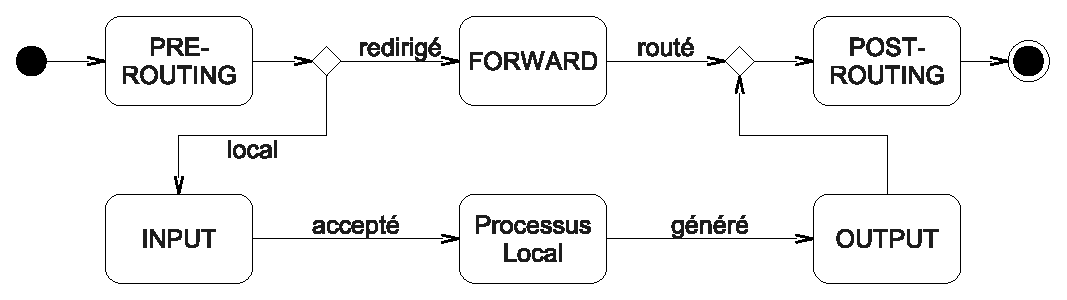
\includegraphics[width=\columnwidth]{firewall}
  \caption{Struktur des Paketfilters}
  \label{fig:netfilter}
\end{figure}

Mit der Paketfilterkonfiguration lassen sich die einzelnen
Ketten des Paketfilters direkt konfigurieren. Dazu gibt es für
jede relevante Kette ein eigenes Array, d.h. eine für die
\fwchain{INPUT}-Kette (\var{PF\_INPUT\_\%}), eine für die
\fwchain{FORWARD}-Kette (\var{PF\_FORWARD\_\%}), eine für die
\fwchain{OUTPUT}-Kette (\var{PF\_OUTPUT\_\%}), eine für die
\fwchain{PREROUTING}-Kette, in der die Portweiterleitung durchgeführt wird
(\var{PF\_PREROUTING\_\%}), und eine für die \fwchain{POSTROUTING}-Kette,
in der das Maskieren der Pakete durchgeführt wird (\var{PF\_POSTROUTING\_\%}).

Ein Eintrag in einem dieser Arrays besteht im
Wesentlichen aus einer Aktion (s.u.),
die durch zusätzliche Bedingungen eingeschränkt werden kann. Diese Bedingungen
beziehen sich auf Eigenschaften des betrachteten Paketes. Ein Paket
enthält Informationen über seine Herkunft (Quelle, welcher Rechner hat
das Paket losgeschickt), sein Ziel (an welchen Rechner und welche
Anwendung soll das Paket gehen) u.a.m. Bedingungen können sich auf
folgende Eigenschaften eines Paketes beziehen:

\begin{itemize}
  \item die Quelle (Quell-Adresse, Quell-Port oder beides)
  \item das Ziel (Ziel-Adresse, Ziel-Port oder beides)
  \item das Protokoll
  \item die Schnittstelle, über welches das Paket hereinkommt bzw. hinausgeht
  \item die MAC-Adresse des Rechners, von dem das Paket kommt
  \item den Zustand des Paketes bzw. der Verbindung, zu der das Paket gehört
\end{itemize}

Kommt ein Paket herein, werden die Einträge bzw. die daraus generierten
Regeln von oben nach unten abgearbeitet und die erste Aktion
ausgeführt, bei der alle Bedingungen gelten.  Trifft keine der Regeln
zu, wird die Standardaktion ausgeführt, die man für (fast) jede
Tabelle angeben kann.

Ein Eintrag hat dabei folgendes Format, wobei zu beachten ist, dass
alle Einschränkungen optional sind:

\begin{example}
\begin{verbatim}
    restriction{0,} [[source] [destination]] action [BIDIRECTIONAL|LOG|NOLOG]
\end{verbatim}
\end{example}

An allen Stellen, an denen Netzwerke, IP-Adressen oder Hosts angegeben werden
müssen, kann man sich auch auf \var{IP\_NET\_\%}, \var{IP\_NET\_\%\_IPADDR} oder
via \host{@hostname} auf einen Host aus \var{HOST\_\%} beziehen. Ist
\var{OPT\_DNS} aktiviert, dann können außerhalb von Aktionen via \host{@fqdn}
auch Hosts über ihren Namen referenziert werden, die \emph{nicht} in
\var{HOST\_\%} zu finden sind. Das ist insbesondere dann sinnvoll, wenn es
sich um externe Hosts handelt, die zudem viele (und wechselnde) IP-Adressen
besitzen.

\marklabel{sec:fwrules_actions}{\subsection{Aktionen des Paketfilters}}

Aktionen können die folgenden sein:
\begin{center}
    \begin{longtable}{|l|l|p{0.5\textwidth}|}
        \hline
        \multicolumn{1}{|l}{\textbf{Aktion}} &
        \multicolumn{1}{|l}{\textbf{Kette(n)}} &
        \multicolumn{1}{|l|}{\textbf{Bedeutung}} \\
        \hline
        \endhead
        \hline
        \endfoot
        \endlastfoot
        \fwaction{ACCEPT}       & alle
                                & Akzeptiere das Paket.
                                \\
        \hline
        \fwaction{DROP}         &
                                \begin{tabular}[t]{@{}l@{}}
                                    \fwchain{INPUT} \\
                                    \fwchain{FORWARD} \\
                                    \fwchain{OUTPUT}
                                \end{tabular}
                                & Verwirf das Paket (der Absender erkennt das
                                nur daran, dass keine Antwort, aber auch keine
                                Fehlermeldung zurückkommt).
                                \\
        \hline
        \fwaction{REJECT}       &
                                \begin{tabular}[t]{@{}l@{}}
                                    \fwchain{INPUT} \\
                                    \fwchain{FORWARD} \\
                                    \fwchain{OUTPUT}
                                \end{tabular}
                                & Weise das Paket zurück (der Absender erhält
                                eine entsprechende Fehlermeldung).
                                \\
        \hline
        \fwaction{LOG}          & alle
                                & Protokolliere das Paket und gehe zur nächsten
                                Regel. Um verschiedene Protokoll-Einträge
                                auseinanderhalten zu können, kann ein Präfix
                                verwendet werden, das via
                                \fwaction{LOG:log-prefix} angegeben wird. Dieses
                                Präfix darf maximal 28 Zeichen lang sein und
                                kann aus Buchstaben, Ziffern, dem Bindestrich
                                (\texttt{-}) und dem Unterstrich (\texttt{\_})
                                bestehen.
                                \\
        \hline
        \fwaction{MASQUERADE}   & \fwchain{POSTROUTING}
                                & Maskiere das Paket: Ersetze die Quelladresse
                                des Paketes durch die eigene, der Schnittstelle
                                zugewiesenen Adresse und sorge dafür, dass
                                Antworten für diese Verbindung an den richtigen
                                Rechner weitergeleitet werden.
                                \\
        \hline
        \fwaction{SNAT}         & \fwchain{POSTROUTING}
                                & Ersetze die Quelladresse und den Quellport
                                des Paketes durch die als Parameter für
                                \fwaction{SNAT} angegebene Adresse (für alle
                                Pakete, die zu der gerade betrachteten
                                Verbindung gehören).
                                \\
        \hline
        \fwaction{DNAT}         & \fwchain{PREROUTING}
                                & Ersetze die Zieladresse und den Zielport des
                                Paketes durch die als Parameter für
                                \fwaction{DNAT} angegebene Adresse (für alle
                                Pakete, die zu der gerade betrachteten
                                Verbindung gehören).
                                \\
        \hline
        \fwaction{REDIRECT}     &
                                \begin{tabular}[t]{@{}l@{}}
                                    \fwchain{PREROUTING} \\
                                    \fwchain{OUTPUT}
                                \end{tabular}
                                & Ersetze den Zielport des Paketes durch den
                                als Parameter für \fwaction{REDIRECT}
                                angegebenen Port und stelle das Paket lokal zu
                                (für alle Pakete, die zu der gerade
                                betrachteten Verbindung gehören).
                                \\
        \hline
        \fwaction{NETMAP}       &
                                \begin{tabular}[t]{@{}l@{}}
                                    \fwchain{PREROUTING} \\
                                    \fwchain{POSTROUTING}
                                \end{tabular}
                                & Bilde die Ziel- bzw. Quelladresse des Paketes
                                in den als Parameter für \fwaction{NETMAP}
                                angegebenen Bereich ab, die Ports bleiben
                                unverändert (für alle Pakete, die zu der gerade
                                betrachteten Verbindung gehören; in der
                                \fwchain{PREROUTING}-Kette wird die Zieladresse
                                verändert, in der \fwchain{POSTROUTING}-Kette
                                die Quelladresse).
                                \\
        \hline
        \caption{Aktionen in Paketfilterregeln}\marklabel{fwrule:actions}{}
    \end{longtable}
\end{center}

Einige dieser Aktionen können durch die Optionen \fwaction{BIDIRECTIONAL},
\fwaction{LOG} oder \fwaction{NOLOG} in ihrem Verhalten modifiziert werden.
\fwaction{BIDIRECTIONAL} generiert die gleiche Regel noch einmal, nur mit
vertauschter Quell- und Zieladresse (und vertauschtem Quell- und Zielport
und/oder vertauschter ein- und ausgehender Netzwerk-Schnittstelle, falls
angegeben). \fwaction{LOG}/\fwaction{NOLOG} aktivieren bzw. deaktivieren das
Protokollieren für diese eine Regel.

\marklabel{sec:fwrules_limits}{\subsection{Einschränkungen in den Regeln}}

Einschränkungen können durch die in den folgenden Abschnitten
aufgeführten Bedingungen vorgenommen werden. Bei den Bedingungen kann
man immer \fwmatch{any} angeben, wenn man an irgendeiner Stelle keine
Einschränkung vornehmen will, aber trotzdem etwas angeben
will/muss. Einschränkungen können in beliebiger Reihenfolge angegeben
werden, wenn sie einen vorangestellten Präfix haben. Das gilt für alle
Einschränkungen, außer für die Angabe einer Quell- bzw. Zieladresse. Diese
müssen immer direkt vor der Aktion stehen, die anderen Einschränkungen müssen
vorher erfolgen. Einschränkungen können auch negiert werden, dazu wird
einfach ein \fwmatch{!} vorangestellt.

\subsubsection{Einschränkungen der Quelle und des Ziels}

Jedes Paket enthält eine Quell- und eine Zielangabe, jeweils in Form
eines Tupels einer IP-Adresse und eines Ports.\footnote{Ein Port ist nur bei
TCP- und UDP-Paketen vorhanden.} Diese Quelle bzw. dieses Ziel kann für eine
Einschränkung herangezogen werden. Die Angabe für die Quelle bzw. das Ziel kann
folgendermaßen vorgenommen werden:

\begin{center}
    \begin{longtable}{|l|p{0.5\textwidth}|}
        \hline
        \multicolumn{1}{|l}{\textbf{Ausdruck}} &
        \multicolumn{1}{|l|}{\textbf{Bedeutung}} \\
        \hline
        \endhead
        \hline
        \endfoot
        \endlastfoot
    \verb+ip+               & eine einfache IP-Adresse\\
    \verb+network+          & eine Netzwerkangabe der Form \verb+<ip>/<netmask>+ \\
    \verb+port[-port]+      & ein Port bzw. ein Port-Bereich\\
    \verb+IP_NET_x_IPADDR+  & die IP-Adresse der Schnittstelle \verb+x+ des Routers\\
    \verb+IP_NET_x+         & das Subnetz \verb+x+ des Routers\\
    \verb+IP_ROUTE_x+       & das in der Route \verb+x+ angegebene Subnetz
      (Default-Routen können nicht verwendet werden, sie würden \fwmatch{any} entsprechen und
      werden vorsichtshalber ausgeklammert)\\
    \verb+@name+            & einer der via HOST\_\%\_* vergebenen Namen oder
      Aliase; es wird die zugehörige IP-Adresse an dieser Stelle eingesetzt\\
    \verb+<ip oder netzwerk>:port[-port]+ & Host- bzw. Netzwerk-Adresse in einer
      der obigen Varianten, kombiniert mit einem Port bzw. Port-Bereich\\
        \hline
        \caption{Quell- und Zieleinschränkungen in Paketfilterregeln}
    \end{longtable}
\end{center}

\noindent Das könnte z.\,B. wie folgt aussehen: \verb+'192.168.6.2 any DROP'+

Tauchen zwei dieser Angaben auf, wird die erste als Quelle, die zweite
als Ziel betrachtet. In diesem Beispiel verwerfen wir also Pakete, die
vom Rechner mit der IP-Adresse 192.168.6.2 gesendet wurden, unabhängig
davon, an welches Ziel sie gerichtet sind.

Taucht nur eine Angabe auf, wird anhand des Wertes entschieden, ob die
Quelle oder das Ziel gemeint ist, wobei die Entscheidung relativ
einfach ist:
\begin{itemize}
  \item Ist eine Port-Angabe enthalten, ist das Ziel gemeint.
  \item Sonst ist die Quelle gemeint.
\end{itemize}

Wenn wir also z.\,B. das obige Beispiel abkürzen wollten,
könnten wir einfach \verb+'192.168.6.2 DROP'+ schreiben. Es ist kein
Port angegeben, die Bedingung gilt also für die Quelle, den Rechner,
von dem das Paket gesendet wurde.

Wollen wir die Kommunikation mit dem \protocol{ssh}-Dämon erlauben, können
wir \verb+'any any:22 ACCEPT'+ (Pakete von einem beliebigen Rechner an den
\protocol{ssh}-Port 22 eines beliebigen Rechners werden akzeptiert) oder
kürzer \verb+'22 ACCEPT'+ schreiben: Es ist nur ein Port angegeben,
also meinen wir das Ziel und damit Pakete, die an den Port 22
gerichtet sind.

Zur Vereinfachung der Regelmenge kann man an die Aktion ein
\fwaction{BIDIRECTIONAL} dranhängen, um auszudrücken, dass die Regel für beide
Kommunikationsrichtungen gilt. Es werden dann Regeln generiert, in
denen einfach die Quell- und die Ziel-Adressen und eventuell angegebenene Ports
und Netzwerk-Schnittstellen vertauscht sind und der Rest gleich bleibt.

Beispiele:
\medskip

\begin{example}
\noindent
{\footnotesize
 \begin{tabular}{@{}p{5cm}p{10cm}@{}}
    \verb+127.0.0.1 ACCEPT+             & Lokale Kommunikation (Quelle 127.0.0.1) ist erlaubt \\
    \verb+any 192.168.12.1 DROP+        & Pakete an die Adresse 192.168.12.1 werden weggeworfen \\
    \verb+any 192.168.12.1 DROP LOG+    & Pakete an die Adresse 192.168.12.1 werden weggeworfen und zusätzlich protokolliert \\
    \verb+any 192.168.12.1 DROP NOLOG+  & Pakete an die Adresse 192.168.12.1 werden weggeworfen, werden aber nicht protokolliert \\
    \verb+22 ACCEPT+                    & Pakete an den Port 22 (\protocol{ssh}) werden akzeptiert \\
    \verb+IP_NET_1_NET ACCEPT+          & Pakete aus dem an der ersten Schnittstelle hängenden Subnetz werden akzeptiert\\
    \verb+IP_NET_1_NET IP_NET_2_NET+    & Kommunikation zwischen den an der ersten und zweiten\\
    \verb+  ACCEPT BIDIRECTIONAL+       & Schnittstelle hängenden Subnetzen ist gestattet
 \end{tabular}
}
\end{example}

\subsubsection{Einschränkung der Schnittstelle}

Eine Regel kann eingeschränkt werden in Bezug auf die Schnittstelle, über die
ein Paket hereinkam bzw. hinausgeht. Das Format sieht wie folgt aus:
\fwmatch{if:}\emph{in}\fwmatch{:}\emph{out}

In der \fwchain{INPUT}-Kette kann man die Schnittstelle für hinausgehende
Pakete nicht einschränken (das Paket geht ja nicht mehr hinaus), in der
\fwchain{POSTROUTING}-Kette kann man die Schnittstelle für hereinkommende
Pakete nicht einschränken, da die Information darüber nicht mehr vorhanden ist.
Lediglich in der \fwchain{FORWARD}-Kette kann man für beides Bedingungen
angeben.

Möglich sind folgende Werte für \emph{in} bzw. \emph{out}:

\begin{itemize}
  \item \fwmatch{lo} (Loopback-Schnittstelle, lokale Kommunikation auf dem
    Router)
  \item \verb+IP_NET_x_DEV+
  \item \fwmatch{pppoe} (die PPPoE-Schnittstelle; nur bei entsprechend
    aktiviertem \package{dsl}- oder \package{pppoe\_server}-Paket)
  \item \fwmatch{any}
\end{itemize}

\subsubsection{Einschränkungen des Protokolls}

Eine Regel kann eingeschränkt werden in Bezug auf das Protokoll, zu dem ein
Paket gehört. Das Format sieht wie folgt aus:
\fwmatch{prot:}\emph{protocol} bzw. \fwmatch{prot:}\emph{icmp}\fwmatch{:}\emph{icmp-type}.
\emph{protocol} kann dabei einen der folgenden Werte annehmen:

\begin{itemize}
  \item \fwmatch{tcp}
  \item \fwmatch{udp}
  \item \fwmatch{gre} (Generic Routing Encapsulation)
  \item \fwmatch{icmp} (hier kann man zusätzlich noch einen Namen für den
    zu filternden ICMP-Typ angeben (\fwmatch{echo-reply} oder
    \fwmatch{echo-request}), etwa \fwmatch{prot:icmp:echo-request})
  \item numerischer Wert der Protokoll-ID (z.\,B. 41 für IPv6)
  \item \fwmatch{any}
\end{itemize}

Wenn eine solche Einschränkung nicht vorhanden ist, aber dennoch Portnummern
in einer Regel verwendet werden, dann wird die Regel \emph{zweimal} angelegt,
nämlich einmal für das \protocol{tcp}- und einmal für das
\protocol{udp}-Protokoll.

\subsubsection{Einschränkung der MAC-Adresse}

Mittels \fwmatch{mac:}\emph{mac-address} kann eine Einschränkung bezüglich der
MAC-Adresse vorgenommen werden.

\subsubsection{Einschränkungen in Bezug auf den Zustand eines Paketes}

Der von fli4l verwendete Paketfilter sammelt Informationen über den
Zustand von Verbindungen. Diese Informationen kann man dann nutzen, um
Pakete zu filtern, also z.\,B. nur Pakete durchzulassen, die zu bereits
bestehenden Verbindungen gehören. Die Zustände einer Verbindung können
sein:\footnote{siehe \altlink{http://www.sns.ias.edu/~jns/files/iptables_talk/x38.htm}
für eine genauere Beschreibung der Zustände}

\begin{center}
    \begin{longtable}{|l|p{0.7\textwidth}|}
        \hline
        \multicolumn{1}{|l}{\textbf{Zustand}} &
        \multicolumn{1}{|l|}{\textbf{Bedeutung}} \\
        \hline
        \endhead
        \hline
        \endfoot
        \endlastfoot
        \fwpktstate{INVALID}        & Das Paket gehört zu keiner bekannten
                                    Verbindung.
                                    \\
        \fwpktstate{ESTABLISHED}    & Das Paket gehört zu einer Verbindung,
                                    über die bereits in beide Richtungen Pakete
                                    geflossen sind.
                                    \\
        \fwpktstate{NEW}            & Das Paket hat eine neue Verbindung
                                    aufgebaut oder gehört zu einer Verbindung,
                                    bei der noch nicht Pakete in beide
                                    Richtungen geflossen sind.
                                    \\
        \fwpktstate{RELATED}        & Das Paket baut eine neue Verbindung auf,
                                    hat aber eine Beziehung zu einer
                                    bestehenden Verbindung (z.\,B. baut
                                    \protocol{ftp} eine separate Verbindung für
                                    den eigentlichen Datentransfer auf).
                                    \\
        \hline
        \caption{Zustandseinschränkungen in Paketfilterregeln}
    \end{longtable}
\end{center}

Die Zustände werden wie folgt angegeben:
\fwmatch{state:}\emph{state(s)}. Will man mehrere
Zustände angeben, werden diese mit Komma getrennt. Um z.\,B. nur Pakete
durchzulassen, die direkt oder indirekt zu bestehenden Verbindungen gehören,
kann man \fwmatch{state:}\fwpktstate{ESTABLISHED,RELATED} schreiben (dies ist
in der \fwchain{INPUT}- oder \fwchain{FORWARD}-Kette sinnvoll).

\subsubsection{Einschränkung der Häufigkeit einer Aktion}

Unter bestimmten Umständen möchte man die Häufigkeit von Aktionen
begrenzen, z.\,B. nur eine ICMP-Echo-Anforderung pro Sekunde zulassen. Das
kann man mit der \fwmatch{limit}-Einschränkung erreichen, die wie folgt
aussieht: \fwmatch{limit:}\emph{Häufigkeit:Burst}. Die
Häufigkeit wird dabei als \emph{n/Zeiteinheit} (second, minute, hour, day)
angegeben, wobei zusätzlich noch Ereignisse gehäuft auftreten
können (Burst). Die Angabe \texttt{limit:3/minute:5} heißt z.\,B., dass
höchstens drei Ereignisse pro Minute erlaubt sind, wobei auch mal fünf
Ereignisse dicht aufeinander folgend akzeptiert werden.

\marklabel{sec:templates}{\subsection{Der Einsatz von Schablonen im Paketfilter}}

Um den Umgang mit dem Paketfilter weiter zu vereinfachen, gibt es die
Möglichkeit, häufig vorkommende Regeln zu sogenannten Schablonen (Templates)
zusammenzufassen. Damit ist es möglich, eine ganze Reihe von
Paketfilterregeln zusammenzufassen und dieser Sammlung von Regeln
einen symbolischen Namen zu geben. Anstatt direkt mit Protokollen und
Portnummern zu hantieren, verwenden Sie dann Einträge wie \fwmatch{tmpl:ssh},
wenn Sie das \protocol{ssh}-Protokoll in einer Regel verwenden wollen. Wie mit
Schablonen zu verfahren ist, wird hier am Beispiel von \protocol{ssh} gezeigt.

Wollen Sie Ihren fli4l-Router vom Internet aus per \protocol{ssh} erreichen, so
schreiben Sie in einen Eintrag der Array-Variable \var{PF\_INPUT\_\%} den
entsprechenden Dienstnamen (hier \protocol{ssh}) mit vorangestelltem
\fwmatch{tmpl:} und der Aktion, die für diesen Dienst gelten soll. Beispiel:

\begin{example}
\begin{verbatim}
    PF_INPUT_2='tmpl:ssh ACCEPT'
\end{verbatim}
\end{example}

Hierbei steht \fwmatch{tmpl:} dafür, dass eine Regel auf einer Schablone
basieren soll. Den Namen des Dienstes geben Sie nach dem `:'
an, in unserem Beispiel also \protocol{ssh}. Zum Schluss geben Sie an, welche
Aktion mit dem Dienst verbunden werden soll. Da Sie den fli4l-Router
aus dem Internet erreichen wollen, erlauben wir die Verbindung mit
\fwaction{ACCEPT}. Einschränkungen von IP-Adressen oder Netzen sind nicht
angegeben, also ist der \protocol{ssh}-Dienst von allen Netzen und über alle
Schnittstellen erreichbar. Sie könnten bei Bedarf die gewohnten Schreibweisen
vom Paketfilter benutzen, um den Zugriff auf den \protocol{ssh}-Dienst weiter
einzuschränken.

Für welche Dienste Regeln vorbereitet sind (d.h. Schablonen existieren),
kann in der Schablonen-Datei in \verb+opt/etc/fwrules.tmpl/templates+
nachgelesen werden. Im Folgenden finden Sie die Aufstellung in Tabellenform
(siehe Tabelle \ref{tab:fwrules_tmpl}).

\begin{center}
  {\footnotesize
  \begin{longtable}{|lll|}
     \hline
     {\textbf{Schablone}} & {\textbf{Protokoll}} & {\textbf{Port(s)}} \\
     \hline\hline
     \endhead
     \input{fwrules_tmpl_table.inc} \\
     \caption{Im Lieferumfang von fli4l enthaltene Schablonen}
     \label{tab:fwrules_tmpl}
  \end{longtable}}
\end{center}

Die Syntax für diese Form der Paketfilterregeln lautet also immer

\begin{example}
\begin{verbatim}
    tmpl:<Name des Dienstes> <Einschränkungen> <Gewünschte Aktion>
\end{verbatim}
\end{example}

wobei als \verb+<Einschränkungen>+ alles erlaubt ist, was unter
\ref{sec:fwrules_limits} beschrieben wird. Die möglichen Werte für
\verb+<Gewünschte Aktion>+ sind in \ref{sec:fwrules_actions} aufgelistet und
beschrieben.

Ein paar weitere Beispiele sollen die Arbeitsweise verdeutlichen. Zuerst
wollen wir uns \var{PF\_PREROUTING} ansehen:

\begin{example}
\begin{verbatim}
    PF_PREROUTING_N='2'
    PF_PREROUTING_1='tmpl:xbl dynamic DNAT:@xbox'
    PF_PREROUTING_2='tmpl:https dynamic DNAT:192.168.193.250'
\end{verbatim}
\end{example}

Die Regel \var{PF\_PREROUTING\_1} versorgt die Xbox mit allem, was für
Xbox Live notwendig ist. Im einzelnen werden mit \fwmatch{tmpl:xbl} alle Ports
und Protokolle, die für Xbox Live notwendig sind, an den Host \host{xbox}
weitergeleitet. Anstelle der IP-Adresse wird ein Eintrag aus dem
\var{HOST\_\%\_NAME}-Array benutzt. Durch \fwmatch{dynamic} weiß der fli4l,
dass die Ports von der Internet-Schnittstelle weitergeleitet werden sollen.

Die zweite Regel leitet das \protocol{https}-Protokoll an einen Webserver in
der DMZ weiter.

Jetzt sehen wir uns an, wie es mit \var{PF\_INPUT} weitergeht:

\begin{example}
\begin{verbatim}
    PF_INPUT_N='3'
    PF_INPUT_1='if:IP_NET_1_DEV:any ACCEPT'
    PF_INPUT_2='if:pppoe:any prot:tcp 113 ACCEPT'
    PF_INPUT_3='if:br0:any tmpl:dns @xbox IP_NET_1_IPADDR ACCEPT'
\end{verbatim}
\end{example}

Die erste Regel lässt alle aus dem Netz, das mit \var{IP\_NET\_1} definiert
ist, auf den Router zugreifen. Die zweite Regel ist für das
\package{oident}-Paket. Dort wird der \protocol{ident}-Port geöffnet. Die
dritte und letzte Regel erlaubt der Xbox den Zugriff auf den DNS Server auf dem
fli4l. Hier ist auch wieder schön zu sehen, wie man einen Host-Alias einsetzt.

In \var{PF\_FORWARD} und \var{PF\_POSTROUTING} steht nichts
\fwmatch{tmpl}-spezifisches mehr.

\begin{figure}[htbp]
  \centering
  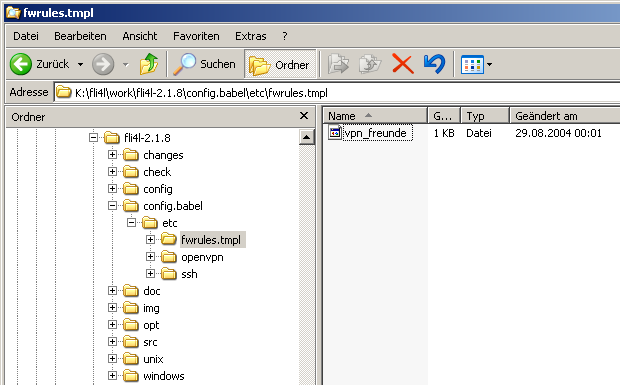
\includegraphics[width=0.9\columnwidth]{etc_fwrules_tmpl_dir}
  \caption{Verzeichnisstruktur fli4l}
  \label{fig:etc_fwrules_tmpl_dir}
\end{figure}

Es ist auch möglich, dass Sie eigene Schablonen anlegen oder dass
Pakete ihre eigenen Schablonen mitbringen. Um eine eigene
Schablone anzulegen, muss lediglich eine Datei mit den Namen der
Schablone erstellt und die entsprechenden Regeln dort
aufgenommen werden. Wenn Sie eine private Schablonendatei anlegen wollen,
erstellen Sie diese in dem Verzeichnis \verb+etc/fwrules.tmpl+ unterhalb Ihres
\texttt{config}-Verzeichnisses, so wie es die Abbildung
\ref{fig:etc_fwrules_tmpl_dir} zeigt. Wenn das Verzeichnis
\texttt{etc/fwrules.tmpl} unterhalb Ihres \texttt{config}-Verzeichnisses noch
nicht existiert, legen Sie bitte zuerst beide Verzeichnisse an. Alternativ
können Paket-Entwickler oder Benutzer, die Schablonen für mehr als eine
Konfiguration anlegen wollen, ihre Regeln direkt in das Verzeichnis
\texttt{opt/etc/fwrules.tmpl} ablegen. In dieses Verzeichnis kommen dann die
neuen Schablonen. Dabei gilt die Regel, dass die Schablonen im
\texttt{config}-Verzeichnis des Benutzers vorrangig behandelt werden.
Zum Schluss wird die Schablonendatei, die zum Lieferumfang von
fli4l gehört, ausgewertet. Sie können also Einträge in der fli4l-Schablonendatei
dadurch \glqq{}überschreiben\grqq{}, indem Sie eine
Schablonendatei mit dem Namen der zu überschreibenden Schablone in Ihrem
\texttt{config}-Verzeichnis anlegen.

Wenn Sie zum Beispiel die Schablone \fwmatch{vpn\_freunde} anlegen wollen, legen
Sie die Datei \texttt{vpn\_freunde} an. Das Template soll die Dienste
\protocol{ssh}, \protocol{smtp}, \protocol{dns} und \protocol{samba} enthalten.
Also schreiben Sie in die Datei \texttt{vpn\_freunde} Folgendes:

\begin{example}
\begin{verbatim}
    prot:tcp 22
    prot:tcp 25
    53
    prot:udp 137-138
    prot:tcp 139
    prot:tcp 445
\end{verbatim}
\end{example}

\noindent Wann immer Sie jetzt die Schablone \fwmatch{vpn\_freunde} benutzen,
werden daraus Regeln für alle darin aufgeführten Protokolle und Ports erzeugt.
\verb+PF_FORWARD_x='tmpl:vpn_freunde ACCEPT'+ etwa erstellt folgende
\fwchain{FORWARD}-Regeln:

\begin{example}
\begin{verbatim}
    prot:tcp 22 ACCEPT
    prot:tcp 25 ACCEPT
    53 ACCEPT
    prot:udp 137-138 ACCEPT
    prot:tcp 139 ACCEPT
    prot:tcp 445 ACCEPT
\end{verbatim}
\end{example}

\subsection{Die Konfiguration des Paketfilters}

Der Paketfilter wird im Wesentlichen durch vier Array-Variablen konfiguriert:

\begin{itemize}
  \item \var{PF\_INPUT\_\%} konfiguriert die \fwchain{INPUT}-Kette,
  \item \var{PF\_FORWARD\_\%} konfiguriert die \fwchain{FORWARD}-Kette,
  \item \var{PF\_OUTPUT\_\%} konfiguriert die \fwchain{OUTPUT}-Kette,
  \item \var{PF\_PREROUTING\_\%} konfiguriert die \fwchain{PREROUTING}-Kette und
  \item \var{PF\_POSTROUTING\_\%} konfiguriert die \fwchain{POSTROUTING}-Kette.
\end{itemize}

\configlabel{PF\_LOG\_LEVEL}{PFLOGLEVEL} Für alle folgenden Ketten
gilt die in \var{PF\_LOG\_LEVEL} vorgenommene Einstellung der
Protokoll-Stufe, deren Inhalt auf einen der folgenden Werte gesetzt werden
kann: \fwloglevel{debug}, \fwloglevel{info}, \fwloglevel{notice},
\fwloglevel{warning}, \fwloglevel{err}, \fwloglevel{crit}, \fwloglevel{alert},
\fwloglevel{emerg}.

\subsubsection{Die \fwchain{INPUT}-Kette}

Über die \fwchain{INPUT}-Kette wird konfiguriert, wer auf den Router zugreifen
darf. Trifft keine der Regeln der \fwchain{INPUT}-Kette zu, bestimmt die
Standard-Aktion, was mit dem Paket passieren soll, und die Protokoll-Variable
bestimmt, ob es bei einer Ablehnung ins System-Protokoll geschrieben werden soll.

Bei den verwendeten Parametern gibt es die folgenden Einschränkungen:
\begin{itemize}
  \item Es können nur \fwaction{ACCEPT}, \fwaction{DROP} und \fwaction{REJECT}
    als Aktion angegeben werden.
  \item Bei einer Schnittstellen-Einschränkung kann man nur die
    Eingangsschnittstelle einschränken.
\end{itemize}

\begin{description}
\config{PF\_INPUT\_POLICY}{PF\_INPUT\_POLICY}{PFINPUTPOLICY}
Diese Variable beschreibt die Standard-Aktion, die angewandt wird,
wenn keine der anderen Regeln zutrifft. Möglich sind:

\begin{itemize}
\item \fwaction{ACCEPT} (nicht empfohlen)
\item \fwaction{REJECT}
\item \fwaction{DROP} (nicht empfohlen)
\end{itemize}

\config{PF\_INPUT\_ACCEPT\_DEF}{PF\_INPUT\_ACCEPT\_DEF}{PFINPUTACCEPTDEF}
Steht diese Variable auf `yes', werden Standard-Regeln generiert, die
für ein korrektes Funktionieren des Routers notwendig
sind. Standardmäßig sollte man hier `yes' eintragen.

Möchte man das Verhalten komplett selbst definieren, kann man
hier `no' eintragen, muss dann jedoch alle Regeln selbst definieren.
Eine zum Standardverhalten äquivalente Konfiguration würde wie folgt
aussehen (die Beschreibung der Liste für benutzerdefinierte Ketten erfolgt
\jump{sec:userlists}{hier}):

\begin{example}
{\footnotesize
\begin{verbatim}
    PF_INPUT_ACCEPT_DEF='no'
    #
    # limit ICMP echo requests - use a separate chain
    #
    PF_USR_CHAIN_N='1'
    PF_USR_CHAIN_1_NAME='usr-in-icmp'
    PF_USR_CHAIN_1_RULE_N='2'
    PF_USR_CHAIN_1_RULE_1='prot:icmp:echo-request length:0-150 limit:1/second:5 ACCEPT'
    PF_USR_CHAIN_1_RULE_2='state:RELATED ACCEPT'

    PF_INPUT_N='4'
    PF_INPUT_1='prot:icmp usr-in-icmp'
    PF_INPUT_2='state:ESTABLISHED,RELATED ACCEPT'
    PF_INPUT_3='if:lo:any ACCEPT'
    PF_INPUT_4='state:NEW 127.0.0.1 DROP BIDIRECTIONAL'
\end{verbatim}}
\end{example}

Die erste Regel verzweigt zur ratenlimitierenden ``usr-in-icmp''-Kette.
Die zweite Regel akzeptiert nur solche Pakete, die zu bestehenden Verbindungen
gehören (also Paketen, die entweder den Zustand \fwpktstate{ESTABLISHED} oder
\fwpktstate{RELATED} besitzen), und die dritte erlaubt lokale Kommunikation
(\verb+if:lo:any ACCEPT+). Die vierte filtert Pakete heraus,
die behaupten, lokale Kommunikation zu sein, aber nicht bereits von
der vorherigen Regel akzeptiert wurden.

Arbeitet man mit OpenVPN, muss man die Regeln
noch ergänzen, um die von diesen Paketen verwendeteten Ketten
einzubinden.

\begin{example}
\begin{verbatim}
    PF_INPUT_N='5'
    ...
    PF_INPUT_5='ovpn-chain'
\end{verbatim}
\end{example}

\config{PF\_INPUT\_LOG}{PF\_INPUT\_LOG}{PFINPUTLOG}
Definiert, ob abgelehnte Pakete vom Kernel protokolliert werden sollen.
Dabei können die Meldungen durch Aktivierung von \var{OPT\_KLOGD} über den
syslog-Dämon entsprechend der Konfiguration ausgegeben werden.

\config{PF\_INPUT\_LOG\_LIMIT}{PF\_INPUT\_LOG\_LIMIT}{PFINPUTLOGLIMIT}
Definiert, wie häufig Log-Einträge generiert werden. Die Häufigkeit
wird analog zur Limit-Einschränkung als \emph{n/Zeiteinheit} mit Bursts
beschrieben, also z.\,B. \texttt{3/minute:5}. Ist dieser Eintrag leer, wird der
Standardwert \texttt{1/second:5} verwendet; enhält er \texttt{none}, wird keine
Limitierung durchgeführt.

\configlabel{PF\_INPUT\_UDP\_REJ\_LIMIT}{PFINPUTUDPREJLIMIT}
\config{PF\_INPUT\_REJ\_LIMIT PF\_INPUT\_UDP\_REJ\_LIMIT}{PF\_INPUT\_REJ\_LIMIT}{PFINPUTREJLIMIT}
Definiert, wie häufig bei einer Ablehnung eines hereinkommenden Paketes
auch ein entsprechendes \fwaction{REJECT}-Paket generiert wird. Die Häufigkeit
wird analog zur Limit-Einschränkung als \emph{n/Zeiteinheit} mit Bursts
beschrieben, also z.\,B. \texttt{3/minute:5}. Ist das Limit überschritten, wird
das Paket einfach ignoriert (\fwaction{DROP}). Ist dieser Eintrag leer, wird
der Standardwert \texttt{1/second:5} verwendet; enhält er \texttt{none}, wird
keine Limitierung durchgeführt.

\config{PF\_INPUT\_ICMP\_ECHO\_REQ\_LIMIT}{PF\_INPUT\_ICMP\_ECHO\_REQ\_LIMIT}{PFINPUTICMPECHOREQLIMIT}
Definiert, wie häufig auf eine ICMP-Echo-Anfrage reagiert werden soll.
Die Häufigkeit wird analog zur Limit-Einschränkung als \emph{n/Zeitein-heit}
mit Bursts beschrieben, also z.\,B. \texttt{/minute:5}. Ist das
Limit überschritten, wird das Paket einfach ignoriert (\fwaction{DROP}). Ist
dieser Eintrag leer, wird der Standardwert \texttt{1/second:5} verwendet;
enhält er \texttt{none}, wird keine Limitierung durchgeführt.

\config{PF\_INPUT\_ICMP\_ECHO\_REQ\_SIZE}{PF\_INPUT\_ICMP\_ECHO\_REQ\_SIZE}{PFINPUTICMPECHOREQSIZE}
Definiert, wie groß eine empfangene ICMP-Echo-Anfrage sein darf (in Bytes). In
dieser Angabe sind neben den ``Nutzdaten'' auch die Paket-Header mit zu
berücksichtigen. Der Standard-Wert liegt bei 150 Bytes.

\configlabel{PF\_INPUT\_x}{PFINPUTx}
\configlabel{PF\_INPUT\_x\_COMMENT}{PFINPUTxCOMMENT}
\config{PF\_INPUT\_N PF\_INPUT\_x PF\_INPUT\_x\_COMMENT}{PF\_INPUT\_N}{PFINPUTN}
Liste der Regeln, die beschreiben, welche Pakete vom Router angenommen
bzw. verworfen werden.
\end{description}

\subsubsection{Die \fwchain{FORWARD}-Kette}

Über die \fwchain{FORWARD}-Kette wird konfiguriert, welche Pakete vom Router
weitergeleitet werden. Trifft keine der Regeln der \fwchain{FORWARD}-Kette zu,
bestimmt die Standard-Aktion, was mit dem Paket passieren soll,und die
Protokoll-Variable bestimmt, ob es bei einer Ablehnung ins System-Protokoll
geschrieben werden soll.

Bei den verwendeten Parametern gibt es die Einschränkung, dass nur
\fwaction{ACCEPT}, \fwaction{DROP} und \fwaction{REJECT} als Aktion angegeben
werden können.

\begin{description}
\config{PF\_FORWARD\_POLICY}{PF\_FORWARD\_POLICY}{PFFORWARDPOLICY}
Diese Variable beschreibt die Standard-Aktion, die angewandt wird,
wenn keine der anderen Regeln zutrifft. Möglich sind:

\begin{itemize}
\item \fwaction{ACCEPT}
\item \fwaction{REJECT}
\item \fwaction{DROP}
\end{itemize}

\config{PF\_FORWARD\_ACCEPT\_DEF}{PF\_FORWARD\_ACCEPT\_DEF}{PFFORWARDACCEPTDEF}
Bestimmt, ob der Router Pakete akzeptiert, die zu bestehenden
Verbindungen gehören. Steht diese Variable auf `yes', generiert fli4l
automatisch eine Regel, die Pakete mit dem entsprechenden Zustand
akzeptiert:

\verb+'state:ESTABLISHED,RELATED ACCEPT'+,

weiterhin eine Regel, die Pakete mit unbekanntem Zustand verwirft:

\verb+'state:INVALID DROP'+.

und schließlich eine Regel, die Pakete mit gefälschten IP-Adressen verwirft:

\verb+'state:NEW 127.0.0.1 DROP BIDIRECTIONAL'+.

Zusätzlich generieren die
anderen Subsysteme auch noch Standardregeln~-- eine Konfiguration ohne
Standardregeln mit Portweiterleitung und OpenVPN würde mindestens
folgende Regeln enthalten:

\begin{example}
\begin{verbatim}
    PF_FORWARD_ACCEPT_DEF='no'
    PF_FORWARD_N='5'
    PF_FORWARD_1='state:ESTABLISHED,RELATED ACCEPT'
    PF_FORWARD_2='state:INVALID DROP'
    PF_FORWARD_3='state:NEW 127.0.0.1 DROP BIDIRECTIONAL'
    PF_FORWARD_4='pfwaccess-chain'
    PF_FORWARD_5='ovpn-chain'
\end{verbatim}
\end{example}

\config{PF\_FORWARD\_LOG}{PF\_FORWARD\_LOG}{PFFORWARDLOG}
Definiert, ob abgelehnte Pakete vom Kernel protokolliert werden sollen.
Dabei können die Meldungen durch Aktivierung von \var{OPT\_KLOGD} über den
syslog-Dämon entsprechend der Konfiguration ausgegeben werden.

\config{PF\_FORWARD\_LOG\_LIMIT}{PF\_FORWARD\_LOG\_LIMIT}{PFFORWARDLOGLIMIT}
Definiert, wie häufig Log-Einträge generiert werden. Die Häufigkeit
wird analog zur Limit-Einschränkung als \emph{n/Zeiteinheit} mit Bursts
beschrieben, also z.\,B. \texttt{3/minute:5}. Ist dieser Eintrag leer, wird der
Standardwert \texttt{1/second:5} verwendet; enhält er \texttt{none}, wird keine
Limitierung durchgeführt.

\configlabel{PF\_FORWARD\_UDP\_REJ\_LIMIT}{PFFORWARDUDPREJLIMIT}
\config{PF\_FORWARD\_REJ\_LIMIT PF\_FORWARD\_UDP\_REJ\_LIMIT}{PF\_FORWARD\_REJ\_LIMIT}{PFFORWARDREJLIMIT}
Definiert, wie häufig bei einer Ablehnung eines hereinkommenden Paketes
auch ein entsprechendes \fwaction{REJECT}-Paket generiert wird. Die Häufigkeit
wird analog zur Limit-Einschränkung als \emph{n/Zeiteinheit} mit Bursts
beschrieben, also z.\,B. \texttt{3/minute:5}. Ist das Limit überschritten, wird
das Paket einfach ignoriert (\fwaction{DROP}). Ist dieser Eintrag leer, wird
der Standardwert \texttt{1/second:5} verwendet; enhält er \texttt{none}, wird
keine Limitierung durchgeführt.

\configlabel{PF\_FORWARD\_x}{PFFORWARDx}
\configlabel{PF\_FORWARD\_x\_COMMENT}{PFFORWARDxCOMMENT}
\config{PF\_FORWARD\_N PF\_FORWARD\_x PF\_FORWARD\_x\_COMMENT}{PF\_FORWARD\_N}{PFFORWARDN}
Liste der Regeln, die beschreiben, welche Pakete vom Router
weitergeleitet bzw. verworfen werden.
\end{description}

\subsubsection{Die \fwchain{OUTPUT}-Kette}

Über die \fwchain{OUTPUT}-Kette wird konfiguriert, worauf der Router selbst
zugreifen darf. Trifft keine der Regeln der \fwchain{OUTPUT}-Kette zu, bestimmt
die Standard-Aktion, was mit dem Paket passieren soll, und die
Protokoll-Variable bestimmt, ob es bei einer Ablehnung ins System-Protokoll
geschrieben werden soll.

Bei den verwendeten Parametern gibt es die folgenden Einschränkungen:
\begin{itemize}
  \item Es können nur \fwaction{ACCEPT}, \fwaction{DROP} und \fwaction{REJECT}
    als Aktion angegeben werden.
  \item Bei einer Schnittstellen-Einschränkung kann man nur die
    Ausgangsschnittstelle einschränken.
\end{itemize}

\begin{description}
\config{PF\_OUTPUT\_POLICY}{PF\_OUTPUT\_POLICY}{PFOUTPUTPOLICY}
Diese Variable beschreibt die Standard-Aktion, die angewandt wird,
wenn keine der anderen Regeln zutrifft. Möglich sind:

\begin{itemize}
\item \fwaction{ACCEPT}
\item \fwaction{REJECT}
\item \fwaction{DROP}
\end{itemize}

\config{PF\_OUTPUT\_ACCEPT\_DEF}{PF\_OUTPUT\_ACCEPT\_DEF}{PFOUTPUTACCEPTDEF}
Steht diese Variable auf `yes', werden Standard-Regeln generiert, die
für ein korrektes Funktionieren des Routers notwendig
sind. Standardmäßig sollte man hier `yes' eintragen.

Möchte man das Verhalten komplett selbst definieren, kann man
hier `no' eintragen, muss dann jedoch alle Regeln selbst definieren.
Eine zum Standardverhalten äquivalente Konfiguration würde wie folgt
aussehen:

\begin{example}
{\footnotesize
\begin{verbatim}
    PF_OUTPUT_ACCEPT_DEF='no'

    PF_OUTPUT_N='1'
    PF_OUTPUT_1='state:ESTABLISHED,RELATED ACCEPT'
\end{verbatim}}
\end{example}

Die erste (und einzige) Regel akzeptiert nur solche Pakete, die zu bestehenden
Verbindungen gehören (also Paketen, die entweder den Zustand
\fwpktstate{ESTABLISHED} oder \fwpktstate{RELATED} besitzen).

\config{PF\_OUTPUT\_LOG}{PF\_OUTPUT\_LOG}{PFOUTPUTLOG}
Definiert, ob abgelehnte Pakete vom Kernel protokolliert werden sollen.
Dabei können die Meldungen durch Aktivierung von \var{OPT\_KLOGD} über den
syslog-Dämon entsprechend der Konfiguration ausgegeben werden.

\config{PF\_OUTPUT\_LOG\_LIMIT}{PF\_OUTPUT\_LOG\_LIMIT}{PFOUTPUTLOGLIMIT}
Definiert, wie häufig Log-Einträge generiert werden. Die Häufigkeit
wird analog zur Limit-Einschränkung als \emph{n/Zeiteinheit} mit Bursts
beschrieben, also z.\,B. \texttt{3/minute:5}. Ist dieser Eintrag leer, wird der
Standardwert \texttt{1/second:5} verwendet; enhält er \texttt{none}, wird keine
Limitierung durchgeführt.

\configlabel{PF\_OUTPUT\_UDP\_REJ\_LIMIT}{PFOUTPUTUDPREJLIMIT}
\config{PF\_OUTPUT\_REJ\_LIMIT PF\_OUTPUT\_UDP\_REJ\_LIMIT}{PF\_OUTPUT\_REJ\_LIMIT}{PFOUTPUTREJLIMIT}
Definiert, wie häufig bei einer Ablehnung eines hereinkommenden Paketes
auch ein entsprechendes \fwaction{REJECT}-Paket generiert wird. Die Häufigkeit
wird analog zur Limit-Einschränkung als \emph{n/Zeiteinheit} mit Bursts
beschrieben, also z.\,B. \texttt{3/minute:5}. Ist das Limit überschritten, wird
das Paket einfach ignoriert (\fwaction{DROP}). Ist dieser Eintrag leer, wird
der Standardwert \texttt{1/second:5} verwendet; enhält er \texttt{none}, wird
keine Limitierung durchgeführt.

\configlabel{PF\_OUTPUT\_x}{PFOUTPUTx}
\configlabel{PF\_OUTPUT\_x\_COMMENT}{PFOUTPUTxCOMMENT}
\config{PF\_OUTPUT\_N PF\_OUTPUT\_x PF\_OUTPUT\_x\_COMMENT}{PF\_OUTPUT\_N}{PFOUTPUTN}
Liste der Regeln, die beschreiben, welche Pakete vom Router versandt
bzw. verworfen werden.
\end{description}

\marklabel{sec:userlists}{\subsubsection{Benutzerdefinierte Listen}}

Aus verschiedenen Gründen besteht manchmal der Bedarf, eigene Ketten
anzulegen und dort die Pakete genauer zu filtern. Diese Ketten kann
man mittels \var{PF\_USR\_CHAIN\_\%} definieren und mit Regeln füllen. Die
Namen der Ketten müssen dabei mit \emph{usr-} beginnen und können nach ihrer
Definition überall in der \fwchain{INPUT}- oder \fwchain{FORWARD}-Kette statt
einer Aktion eingesetzt werden. Als Beispiel soll hier die bereits vorher
verwendete ICMP-Filterkette dienen:

\begin{example}
{\footnotesize
\begin{verbatim}
    PF_USR_CHAIN_N='1'
    #
    # create usr-in-icmp
    #
    PF_USR_CHAIN_1_NAME='usr-in-icmp'
    #
    # add rule to usr-in-icmp
    #
    PF_USR_CHAIN_1_RULE_N='2'
    PF_USR_CHAIN_1_RULE_1='prot:icmp:echo-request length:0-150 limit:1/second:5 ACCEPT'
    PF_USR_CHAIN_1_RULE_2='state:RELATED ACCEPT'
    #
    # use chain in PF_INPUT
    #
    PF_INPUT_2='prot:icmp usr-in-icmp'
\end{verbatim}}
\end{example}

\begin{description}
\config{PF\_USR\_CHAIN\_N}{PF\_USR\_CHAIN\_N}{PFUSRCHAINN} Definiert die Anzahl
der benutzerdefinierten Ketten.

\config{PF\_USR\_CHAIN\_x\_NAME}{PF\_USR\_CHAIN\_x\_NAME}{PFUSRCHAINxNAME}
Definiert den Namen der benutzerdefinierten Kette. Dieser muss mit \emph{usr-}
beginnen.

\configlabel{PF\_USR\_CHAIN\_x\_RULE\_x}{PFUSRCHAINxRULEx}
\configlabel{PF\_USR\_CHAIN\_x\_RULE\_x\_COMMENT}{PFUSRCHAINxRULExCOMMENT}
\config{PF\_USR\_CHAIN\_x\_RULE\_N}{PF\_USR\_CHAIN\_x\_RULE\_N}{dummy0}
\config{PF\_USR\_CHAIN\_x\_RULE\_x}{PF\_USR\_CHAIN\_x\_RULE\_N}{dummy1}
\config{PF\_USR\_CHAIN\_x\_RULE\_x\_COMMENT}{PF\_USR\_CHAIN\_x\_RULE\_N}{PFUSRCHAINxRULEN}
Hier werden die Regeln definiert, die in die benutzerdefinierte Kette
eingefügt werden sollen. Es können alle Regeln verwendet werden, die
auch in einer \fwchain{FORWARD}-Kette verwendet werden könnten.
Sollte keine Regel der benutzerdefinierten Kette zutreffen, wird zur
Ausgangskette zurückgekehrt und mit der Regel nach der Verzweigung fortgefahren.
\end{description}

\subsubsection{Die NAT-Ketten (Network Address Translation)}

Pakete können vor und nach Routing-Entscheidungen noch manipuliert
werden. Sie können zum Beispiel eine neue Zieladresse erhalten, um an einen
anderen Rechner weitergeleitet zu werden (Portweiterleitung) oder eine
andere Quelladresse erhalten, um das hinter dem Router liegende
Netzwerk zu maskieren. Maskieren nutzt man beispielsweise, um ein privates Netz
über eine öffentliche IP ins Netz zu bringen oder in einem DMZ-Setup
die Struktur des lokalen Netzes vor den Rechnern in der DMZ zu
verbergen.

Die Konfiguration erfolgt über zwei Ketten, die \fwchain{PREROUTING}- und die
\fwchain{POSTROUTING}-Kette. Über die \fwchain{POSTROUTING}-Kette wird
konfiguriert, welche Pakete vom Router maskiert werden. Trifft keine der Regeln
der \fwchain{POSTROUTING}-Kette zu, werden die Pakete unmaskiert
weitergeleitet. 

Beim Maskieren gibt es zwei Varianten: eine für Netzwerk-Schnittstellen, die
bei der Einwahl erst eine IP-Adresse zugewiesen bekommen
(\fwaction{MASQUERADE}) und eine für Netzwerk-Schnittstellen mit statischer
IP-Adresse (\fwaction{SNAT}). \fwaction{SNAT} erwartet dabei zusätzlich die
IP-Adresse, die im Paket als Quelle eingetragen werden soll. Diese kann als
\begin{itemize}
\item IP-Adresse (Beispiel: \fwaction{SNAT:1.2.3.4}),
\item IP-Bereich (Beispiel: \fwaction{SNAT:1.2.3.4-1.2.3.10})
\item oder als symbolische Referenz (Beispiel:
\fwaction{SNAT:IP\_NET\_1\_IPADDR})
\end{itemize}
angegeben werden.

Sowohl bei \fwaction{SNAT} als auch bei \fwaction{MASQUERADE} kann schließlich
ein Port bzw. Portbereich angegeben werden, auf den der
Quellport abgebildet werden soll. Normalerweise ist das nicht nötig,
da der Kern die Ports allein auswählen kann. Es gibt aber
Anwendungen, die verlangen, dass der Quellport unverändert bleibt
(und somit ein 1:1-NAT erfordern) oder die ein PAT (Port Address Translation)
oder NAPT (Network Address and Port Translation) verbieten. Der Portbereich wird
einfach hinten angehängt, z.\,B. so:
\fwaction{SNAT:IP\_NET\_1\_IPADDR:4000-8000}.

Bei der \fwchain{POSTROUTING}-Kette können nur \fwaction{ACCEPT},
\fwaction{SNAT}, \fwaction{NETMAP} und \fwaction{MASQUERADE} als Aktionen
verwendet werden.

\begin{description}

\configlabel{PF\_POSTROUTING\_x}{PFPOSTROUTINGx}
\configlabel{PF\_POSTROUTING\_x\_COMMENT}{PFPOSTROUTINGxCOMMENT}
\config{PF\_POSTROUTING\_N PF\_POSTROUTING\_x PF\_POSTROUTING\_x\_COMMENT}{PF\_POSTROUTING\_N}{PFPOSTROUTINGN}
\mbox{}\newline
Eine Liste der Regeln, die beschreiben, welche Pakete vom Router maskiert
werden (bzw. unmaskiert weitergeleitet werden). Will man Pakete vom
Maskieren ausklammern, kann man eine ACCEPT-Regel für die
auszuklammernden Pakete der MASQUERADE-Regel voranstellen.

\end{description}

Über die \fwchain{PREROUTING}-Kette wird konfiguriert, welche Pakete an einen
anderen Rechner weitergeleitet werden sollen. Trifft keine der Regeln
der \fwchain{PREROUTING}-Kette zu, werden die Pakete unverändert
weiterbehandelt. Die Aktion \fwaction{DNAT} erwartet dabei die IP-Adresse, die
im Paket als Ziel eingetragen werden soll. Diese kann als
\begin{itemize}
\item IP-Adresse (Beispiel: \fwaction{DNAT:1.2.3.4}),
\item IP-Bereich (Beispiel: \fwaction{DNAT:1.2.3.4-1.2.3.10})
\item oder als Hostname (Beispiel: \fwaction{DNAT:@client1})
\end{itemize}
angegeben werden.

Schließlich kann noch ein Port bzw. Portbereich angegeben werden, auf den der
Zielport abgebildet werden soll. Das ist aber nur nötig, wenn der Port geändert
werden soll. Der Port bzw. Portbereich wird einfach hinten angehängt, z.\,B.
so:
\fwaction{DNAT:@server:21}.

\fwaction{REDIRECT} verhält sich wie \fwaction{DNAT}, nur dass die
Ziel-IP-Adresse immer auf die (primäre) IP-Adresse der Schnittstelle, auf der das
Paket hereinkam, gesetzt wird und damit das Paket lokal zugestellt wird. Dies
wird z.\,B. für transparente Proxys benötigt, siehe
\jump{OPTTRANSPROXY}{\var{OPT\_TRANSPROXY}}.

Will man eine Portweiterleitung auf Schnittstellen mit dynamischen Adressen
machen, weiß man zum Zeitpunkt der Konfiguration noch nicht, an welche IP die
Pakete gerichtet sein werden. Daher kann man in der \fwchain{PREROUTING}-Kette
\fwmatch{dynamic} als Platzhalter für die später zugewiesene IP verwenden, etwa
wie folgt:

\begin{example}
{\footnotesize
\begin{verbatim}
    'dynamic:80  DNAT:1.2.3.4'           # leite http-Pakete an die
                                         # IP-Adresse 1.2.3.4 weiter
    'prot:gre any dynamic DNAT:1.2.3.4'  # leite gre-Pakete (Teil des PPTP-
                                         # Protokolls) an die IP-Adresse
                                         # 1.2.3.4 weiter
\end{verbatim}}
\end{example}

Bei der \fwchain{PREROUTING}-Kette können nur \fwaction{ACCEPT},
\fwaction{DNAT}, \fwaction{NETMAP} und \fwaction{REDIRECT} als Aktionen
verwendet werden.

Für weitere Beispiele zur Portweiterleitung siehe den nächsten Abschnitt.

\begin{description}

\configlabel{PF\_PREROUTING\_x}{PFPREROUTINGx}
\configlabel{PF\_PREROUTING\_x\_COMMENT}{PFPREROUTINGxCOMMENT}
\config{PF\_PREROUTING\_N PF\_PREROUTING\_x PF\_PREROUTING\_x\_COMMENT}{PF\_PREROUTING\_N}{PFPREROUTINGN}
\mbox{}\newline
Eine Liste der Regeln, die beschreiben, welche Pakete vom Router an ein
anderes Ziel weitergeleitet werden sollen.

\end{description}

\subsection{Beispiele}

Im Folgenden sind einige Beispiele für die Paketfilter-Konfiguration angegeben.

\subsubsection{Die fli4l-Standardkonfiguration}

Die fli4l-Standardkonfiguration der Distribution sieht für die
\fwchain{INPUT}-Kette wie folgt aus:

\begin{example}
\begin{verbatim}
    PF_INPUT_POLICY='REJECT'
    PF_INPUT_ACCEPT_DEF='yes'
    PF_INPUT_LOG='no'
    PF_INPUT_N='1'
    PF_INPUT_1='IP_NET_1 ACCEPT'
\end{verbatim}
\end{example}

Damit erreichen wir, dass
\begin{itemize}
\item Rechner im lokalen Netzwerk auf den Router zugreifen dürfen\\
(\verb+PF_INPUT_1='IP_NET_1 ACCEPT'+),
\item lokale Kommunikation auf dem Router erlaubt ist
  (\verb+PF_INPUT_ACCEPT_DEF='yes'+),
\item Pakete, die zu vom Router aufgebauten Verbindungen gehören,
  akzeptiert werden \newline (\verb+PF_INPUT_ACCEPT_DEF='yes'+),
\item alles andere abgelehnt wird (\verb+PF_INPUT_POLICY='REJECT'+),
\item aber nicht ins System-Protokoll geschrieben wird
  (\verb+PF_INPUT_LOG='no'+).
\end{itemize}

Für die \fwchain{FORWARD}-Kette sieht das so ähnlich aus: Nur Pakete unseres
lokalen Netzes und Pakete, die zu Verbindungen gehören, die von
Rechnern im lokalen Netz aufgebaut wurden, sollen weitergeleitet
werden. Des Weiteren werden NetBIOS- und CIFS-Pakete verworfen.

\begin{example}
\begin{verbatim}
    PF_FORWARD_POLICY='REJECT'
    PF_FORWARD_ACCEPT_DEF='yes'
    PF_FORWARD_LOG='no'
    PF_FORWARD_N='2'
    PF_FORWARD_1='tmpl:samba DROP'
    PF_FORWARD_2='IP_NET_1 ACCEPT'
\end{verbatim}
\end{example}

Was man hier gut sieht, ist die Abhängigkeit von der Reihenfolge der
Regeln: \emph{Zuerst} werden NetBIOS-Pakete verworfen, und \emph{danach} werden
die Pakete des lokalen Netzes akzeptiert.

Nun kann das lokale Netz mit dem Router kommunizieren, seine Pakete
werden weitergeleitet, es fehlt nur noch das Maskieren, welches für
den Zugriff eines privaten Netzwerkes auf das Internet notwendig ist:

\begin{example}
\begin{verbatim}
    PF_POSTROUTING_N='1'
    PF_POSTROUTING_1='IP_NET_1 MASQUERADE'
\end{verbatim}
\end{example}

\subsubsection{Trusted Nets}

Wollen wir lokal mehrere Subnetze haben, die frei und unmaskiert
miteinander kommunizieren können, müssen wir dafür sorgen, dass Pakete
zwischen diesen Subnetzen nicht verworfen und auch nicht maskiert
werden. Dazu fügen wir einfach eine Regel hinzu oder modifizieren die vorhandene.

Angenommen, wir haben einen DSL-Zugang über PPPoE, und die beiden Subnetze sind
\var{IP\_NET\_1} (192.168.6.0/24) und \var{IP\_NET\_2} (192.168.7.0/24).
Dann würde die Konfiguration wie folgt aussehen:

\begin{example}
\begin{verbatim}
    PF_FORWARD_POLICY='REJECT'
    PF_FORWARD_ACCEPT_DEF='yes'
    PF_FORWARD_LOG='no'
    PF_FORWARD_N='4'
    PF_FORWARD_1='IP_NET_1 IP_NET_2 ACCEPT BIDIRECTIONAL'
    PF_FORWARD_2='tmpl:samba DROP'
    PF_FORWARD_3='IP_NET_1 ACCEPT'
    PF_FORWARD_4='IP_NET_2 ACCEPT'

    PF_POSTROUTING_N='3'
    PF_POSTROUTING_1='IP_NET_1 IP_NET_2 ACCEPT BIDIRECTIONAL'
    PF_POSTROUTING_2='IP_NET_1 MASQUERADE'
    PF_POSTROUTING_3='IP_NET_2 MASQUERADE'
\end{verbatim}
\end{example}

Regel eins sorgt jetzt dafür, dass Pakete zwichen den beiden
Subnetzen ohne weitere Prüfung weitergeleitet werden. Die Regeln drei und vier
sorgen dafür, dass beide Subnetze auch ins Internet kommen. Die erste Regel
der \fwchain{POSTROUTING}-Kette sorgt dafür, dass die Kommunikation zwischen
den Subnetzen unmaskiert erfolgt.

Alternativ könnten wir auch sagen, dass nur Pakete, die über die
\fwmatch{pppoe}-Schnittstelle hinausgehen, maskiert werden sollen:

\begin{example}
\begin{verbatim}
    PF_POSTROUTING_N='1'
    PF_POSTROUTING_1='if:any:pppoe MASQUERADE'
\end{verbatim}
\end{example}

Genauso hätte man die Filterung der Ports auch auf die
\fwmatch{pppoe}-Schnittstelle beschränken und die beiden Subnetze zu einem
zusammenfassen können, das würde dann wie folgt aussehen:

\begin{example}
\begin{verbatim}
    PF_FORWARD_POLICY='REJECT'
    PF_FORWARD_ACCEPT_DEF='yes'
    PF_FORWARD_LOG='no'
    PF_FORWARD_N='2'
    PF_FORWARD_1='if:any:pppoe tmpl:samba DROP'
    PF_FORWARD_2='192.168.6.0/23 ACCEPT'

    PF_POSTROUTING_N='1'
    PF_POSTROUTING_1='if:any:pppoe MASQUERADE'
\end{verbatim}
\end{example}

Pakete, die über die \fwmatch{pppoe}-Schnittstelle hinausgehen und die an die
\protocol{udp}-Ports 137-138 oder an die \protocol{tcp}-Ports 139 und 445
adressiert sind, werden verworfen (Regel~1), alle anderen Pakete, die aus dem
Subnetz 192.168.6.0/23 kommen, werden weitergeleitet (Regel~2).

\subsubsection{Route Network}

Fügen wir dem Ganzen noch ein Netzwerk 10.0.0.0/24 hinzu (z.\,B. ein
Dial-In-Netzwerk), mit dem wir unmaskiert kommunizieren wollen, wobei
Pakete an die \protocol{udp}-Ports 137-138 sowie an die \protocol{tcp}-Ports
139 und 445 verworfen werden sollen, dann würde das wie folgt aussehen:

\begin{example}
\begin{verbatim}
    PF_FORWARD_POLICY='REJECT'
    PF_FORWARD_ACCEPT_DEF='yes'
    PF_FORWARD_LOG='no'
    PF_FORWARD_N='4'
    PF_FORWARD_1='IP_NET_1 IP_NET_2 ACCEPT BIDIRECTIONAL'
    PF_FORWARD_2='tmpl:samba DROP'
    PF_FORWARD_3='192.168.6.0/23 ACCEPT'
    PF_FORWARD_4='10.0.0.0/24 ACCEPT'

    PF_POSTROUTING_N='2'
    PF_POSTROUTING_1='10.0.0.0/24 ACCEPT BIDIRECTIONAL'
    PF_POSTROUTING_2='192.168.6.0/23 MASQUERADE'
\end{verbatim}
\end{example}

\begin{itemize}
\item Regel~1 erlaubt die ungehinderte Kommunikation zwischen den Subnetzen
  \var{IP\_NET\_1} und \var{IP\_NET\_2}.
\item Regel~2 verwirft Pakete an die Samba-Ports.
\item Die Regeln 3 und 4 erlaubt die Weiterleitung von Paketen, die aus den
  Subnetzen 192.168.6.0/24, 192.168.7.0/24 und 10.0.0.0/24 kommen; die
  Rückrichtung wird von der Einstellung \verb+PF_FORWARD_ACCEPT_DEF='yes'+
  abgedeckt.
\item Regel~1 der \fwchain{POSTROUTING}-Kette sorgt dafür, dass Pakete in
das bzw. aus dem 10.0.0.0/24-Subnetz nicht maskiert werden.
\end{itemize}

Alternativ ginge auch:

\begin{example}
\begin{verbatim}
    PF_POSTROUTING_N='1'
    PF_POSTROUTING_1='if:any:pppoe MASQUERADE'
\end{verbatim}
\end{example}

Diese Regel besagt, dass nur Pakete, die über die \fwmatch{pppoe}-Schnittstelle
hinausgehen, maskiert werden.

\subsubsection{Blacklists, Whitelists}

Blacklists (ein Rechner in dieser Liste darf etwas nicht) und
Whitelists (ein Rechner in dieser Liste darf etwas) werden prinzipiell
ähnlich umgesetzt. Es werden Regeln geschrieben, die am Anfang sehr
speziell sind und nach hinten immer allgemeiner werden. Bei einer
Blacklist stehen am Anfang Regeln, die etwas verbieten und am Ende
Regeln, die allen bisher nicht erwähnten etwas erlauben. Bei einer
Whitelist ist es genau umgekehrt.

\emph{Beispiel~1:} Alle Rechner im Subnetz 192.168.6.0/24 außer Rechner 12
dürfen ins Internet, solange sie nicht mit den CIFS Ports 137-138
(\protocol{udp}), 139 und 445 (\protocol{tcp}) kommunizieren wollen:

\begin{example}
\begin{verbatim}
    PF_FORWARD_POLICY='REJECT'
    PF_FORWARD_ACCEPT_DEF='yes'
    PF_FORWARD_LOG='no'
    PF_FORWARD_N='3'
    PF_FORWARD_1='192.168.6.12 DROP'
    PF_FORWARD_2='tmpl:samba DROP'
    PF_FORWARD_3='192.168.6.0/23 ACCEPT'

    PF_POSTROUTING_N='1'
    PF_POSTROUTING_2='192.168.6.0/24 MASQUERADE'
\end{verbatim}
\end{example}

\emph{Beispiel~2:} Nur Rechner 12 darf ins Internet (aber nicht an die o.\,g.
Ports \ldots), alle anderen dürfen nur lokal mit einem anderen Subnetz
kommunizieren:

\begin{example}
\begin{verbatim}
    PF_FORWARD_POLICY='REJECT'
    PF_FORWARD_ACCEPT_DEF='yes'
    PF_FORWARD_LOG='no'
    PF_FORWARD_N='3'
    PF_FORWARD_1='192.168.6.0/24 192.168.7.0/24 ACCEPT BIDIRECTIONAL'
    PF_FORWARD_2='tmpl:samba DROP'
    PF_FORWARD_3='192.168.6.12 ACCEPT'

    PF_POSTROUTING_N='1'
    PF_POSTROUTING_1='if:any:pppoe MASQUERADE'
\end{verbatim}
\end{example}

\subsection{Standardkonfigurationen}

\subsubsection{Einfacher maskierender Router mit einem Netz dahinter}

\begin{example}
\begin{verbatim}
#
# Zugriff auf den Router
#
PF_INPUT_POLICY='REJECT'
PF_INPUT_ACCEPT_DEF='yes'
PF_INPUT_LOG='no'
PF_INPUT_N='1'
PF_INPUT_1='IP_NET_1 ACCEPT'   # alle Hosts im lokalen Netz dürfen
                               # auf den Router zugreifen

#
# Zugriff auf das ``Internet''
#
PF_FORWARD_POLICY='REJECT'
PF_FORWARD_ACCEPT_DEF='yes'
PF_FORWARD_LOG='no'

PF_FORWARD_N='2'
PF_FORWARD_1='tmpl:samba DROP' # Samba-Pakete, die das Netz
                               # verlassen wollen, werden verworfen
PF_FORWARD_2='IP_NET_1 ACCEPT' # alle anderen Pakete dürfen das
                               # lokale Netz verlassen

#
# Maskieren des lokalen Netzes
#
PF_POSTROUTING_N='1'
PF_POSTROUTING_1='IP_NET_1 MASQUERADE'  # maskiere Pakete, die das Subnetz
                                        # verlassen
\end{verbatim}
\end{example}

\subsubsection{Einfacher maskierender Router mit zwei Netzen dahinter}

\begin{example}
\begin{verbatim}
#
# Zugriff auf den Router
#
PF_INPUT_POLICY='REJECT'
PF_INPUT_ACCEPT_DEF='yes'
PF_INPUT_LOG='no'
PF_INPUT_N='2'
PF_INPUT_1='IP_NET_1 ACCEPT'   # alle Hosts im lokalen Netz dürfen
                               # auf den Router zugreifen
PF_INPUT_2='IP_NET_2 ACCEPT'   # alle Hosts im lokalen Netz dürfen
                               # auf den Router zugreifen

#
# Zugriff auf das ``Internet''
#
PF_FORWARD_POLICY='REJECT'
PF_FORWARD_ACCEPT_DEF='yes'
PF_FORWARD_LOG='no'

#
# Freie Kommunikation zwischen den Netzen
#
PF_FORWARD_N='4'
PF_FORWARD_1='IP_NET_1 IP_NET_2 ACCEPT BIDIRECTIONAL'
PF_FORWARD_2='tmpl:samba DROP' # Samba-Pakete, die das Netz
                               # verlassen wollen, werden verworfen
PF_FORWARD_3='IP_NET_1 ACCEPT' # alle anderen Pakete dürfen das
                               # lokale Netz verlassen
PF_FORWARD_4='IP_NET_2 ACCEPT' # alle anderen Pakete dürfen das
                               # lokale Netz verlassen

#
# Maskieren der lokalen Netze, unmaskierte Kommunikation zwischen den
# Netzen
#
PF_POSTROUTING_N='3'
PF_POSTROUTING_1'IP_NET_1 IP_NET_2 ACCEPT BIDIRECTIONAL'
PF_POSTROUTING_2='IP_NET_1 MASQUERADE'  # maskiere Pakete, die das Subnetz
                                        # verlassen
PF_POSTROUTING_3='IP_NET_2 MASQUERADE'  # maskiere Pakete, die das Subnetz
                                        # verlassen
\end{verbatim}
\end{example}

\subsubsection{Maskierender DSL-Router mit zwei Netzen dahinter und
SSH/HTTP-Zugriff aus dem Internet}

\begin{example}
\begin{verbatim}
#
# Zugriff auf den Router
#
PF_INPUT_POLICY='REJECT'
PF_INPUT_ACCEPT_DEF='yes'
PF_INPUT_LOG='no'
PF_INPUT_N='4'
PF_INPUT_1='IP_NET_1 ACCEPT'   # alle Hosts im lokalen Netz dürfen
                               # auf den Router zugreifen
PF_INPUT_2='IP_NET_2 ACCEPT'   # alle Hosts im lokalen Netz dürfen
                               # auf den Router zugreifen
PF_INPUT_3='tmpl:ssh ACCEPT'   # gestatte Zugriff auf SSH-Dienst
                               # von überall her
PF_INPUT_4='tmpl:http 1.2.3.4/24 ACCEPT'  # gestatte Rechner aus
                               # einem bestimmten Subnetz Zugriff
                               # auf HTTP-Dienst


#
# Zugriff auf das ``Internet''
#
PF_FORWARD_POLICY='REJECT'
PF_FORWARD_ACCEPT_DEF='yes'
PF_FORWARD_LOG='no'

#
# Keine Kommunikation zwischen den Netzen, beide Netze dürfen ins
# Internet, Samba-Pakete werden verworfen
#
PF_FORWARD_N='2'
PF_FORWARD_1='tmpl:samba if:any:pppoe DROP' # Samba-Pakete, die das Netz
                               # verlassen wollen, werden verworfen
PF_FORWARD_2='if:any:pppoe ACCEPT' # alle anderen Pakete dürfen das
                               # lokale Netz verlassen

#
# Maskieren der lokalen Netze, unmaskierte Kommunikation zwischen den
# Netzen
#
PF_POSTROUTING_N='1'
PF_POSTROUTING_1='if:any:pppoe MASQUERADE'  # maskiere Pakete, die das Subnetz
                                            # verlassen
\end{verbatim}
\end{example}

\subsubsection{Portweiterleitung}

Portweiterleitungen lassen sich mit den \fwchain{PREROUTING}-Regeln wie folgt
umsetzen (\verb+TARGET+ bezeichnet die ursprüngliche Zieladresse (optional) und
den ursprünglichen Zielport, \verb+NEW_TARGET+ bezeichnet die neue Zieladresse
und den neuen Zielport (optional), \verb+PROTOCOL+ bezeichnet das jeweilige
Protokoll):

\begin{example}
\begin{verbatim}
    TARGET='<port>'
    NEW_TARGET='<ip>'
    PROTOCOL='<proto>'
    PF_PREROUTING_x='prot:<proto> dynamic:<port> DNAT:<ip>'

    TARGET='<port1>-<port2>'
    NEW_TARGET='<ip>'
    PROTOCOL='<proto>'
    PF_PREROUTING_x='prot:<proto> dynamic:<port1>-<port2> DNAT:<ip>'

    TARGET='<ip>:<port-a>'
    NEW_TARGET='<ip>:<port-b>'
    PROTOCOL='<proto>'
    PF_PREROUTING_x='prot:<proto> any <ip>:<port-a> DNAT:<ip>:<port-b>'
\end{verbatim}
\end{example}

\subsubsection{Transparenter Proxy}
Will man bestimmte Zugriffe auf das Internet nur über einen lokalen Proxy
zulassen, kann man das mit Hilfe der \fwchain{PREROUTING}- und
\fwchain{POSTROUTING}-Ketten erzwingen, ohne dass der Client davon etwas merkt.
Prinzipiell sind dazu drei Schritte notwendig:

\begin{enumerate}
\item Anfragen an den HTTP-Port, die nicht vom Proxy kommen, an den
Proxy umleiten (\fwchain{PREROUTING}).
\item Die umgeleiteten Pakete so verändern, dass der Proxy denkt, sie
kommen vom Router, so dass er sie wieder dorthin zurückschickt
(\fwchain{POSTROUTING}).
\item Die Pakete durch die FORWARD-Kette durchlassen, sofern ein
Eintrag à la

\begin{example}
\begin{verbatim}
PF_FORWARD_x='IP_NET_1 ACCEPT'
\end{verbatim}
\end{example}

nicht existiert (\fwchain{FORWARD}).
\end{enumerate}

\emph{Beispiel~1:} Angenommen, wir haben nur ein Netz \var{IP\_NET\_1},
in dem auf einem Rechner namens \host{proxy} ein Squid-Proxy läuft, und
wollen den gesamten \protocol{http}-Datenverkehr über ihn leiten. Squid lauscht
auf Port 3128. Der Einfachheit halber beziehen wir uns via \host{@proxy} auf
den eingetragenen Host aus \verb+HOST_1_NAME='proxy'+ (vgl.
\jump{sec:domainkonfiguration}{Domainkonfiguration}).

Das Ganze würde wie folgt aussehen:

\begin{example}
\begin{verbatim}
...
  PF_PREROUTING_x='@proxy ACCEPT'
      # Pakete vom Proxy sollen nicht umgeleitet werden

  PF_PREROUTING_x='prot:tcp IP_NET_1 80 DNAT:@proxy:3128'
      # HTTP-Pakete aus IP_NET_1 mit einem beliebigen Ziel werden
      # umgeleitet nach @proxy, Port 3128

  PF_POSTROUTING_x='any @proxy:3128 SNAT:IP_NET_1_IPADDR'
      # alle Pakete an den Proxy-Port 3128 so umschreiben, als wären sie
      # vom fli4l (IP_NET_1_IPADDR)

  PF_FORWARD_x='prot:tcp @proxy 80 ACCEPT'
      # HTTP-Pakete vom Proxy durch die FORWARD-Kette durchlassen (wenn nötig)
...
\end{verbatim}
\end{example}

Gibt es mehrere Netze oder potentielle Konflikte mit anderen
Portweiterleitungen (die ja auch nichts anderes sind als
\fwaction{DNAT}-Regeln), muss man die Regeln vielleicht noch etwas enger
formulieren.

\emph{Beispiel~2:} Unser Proxy namens \host{proxy} steht in \var{IP\_NET\_1},
lauscht auf Port 3128 und soll nur für Clients aus \var{IP\_NET\_1} wirksam
werden. \var{IP\_NET\_1} ist über \var{IP\_NET\_1\_DEV} erreichbar. Pakete aus
weiteren Netzen sollen nicht berücksichtigt werden.

\begin{example}
\begin{verbatim}
...
  PF_PREROUTING_x='if:IP_NET_1_DEV:any !@proxy 80 DNAT:@proxy:3128'
      # Anfragen an den HTTP-Port, die nicht vom Proxy, aber über eine
      # interne Schnittstelle (IP_NET_1_DEV) kommen, an den Proxy-Port umleiten.
      # An dieser Stelle ist es wichtig, mit if:IP_NET_1_DEV:any zu
      # überprüfen, ob die Pakete von innen kommen, da sonst auch Pakete von
      # außen umgeleitet würden (Sicherheitslücke!).

  PF_POSTROUTING_x='prot:tcp IP_NET_1 @proxy:3128 SNAT:IP_NET_1_IPADDR'
      # HTTP-Pakete die aus IP_NET_1 stammen und für den Proxy-Port 3128
      # gedacht sind, so umschreiben, als wären sie vom fli4l (IP_NET_1_IPADDR)

  PF_FORWARD_x='prot:tcp @proxy 80 ACCEPT'
      # HTTP-Pakete vom Proxy durch die FORWARD-Kette durchlassen (wenn nötig)
...
\end{verbatim}
\end{example}

\emph{Beispiel~3:} Um sich das Leben etwas zu erleichtern und die Regeln
kürzer zu gestalten, kann man auch Templates einsetzen (vgl.
\jump{sec:templates}{Templates im Paketfilter}). Zweckmäßig ist an dieser
Stelle das \fwmatch{tmpl:http}, das in \fwmatch{prot:tcp any any:80}
übersetzt wird. So wird z.\,B. aus \fwmatch{tmpl:http IP\_NET\_1 DNAT:@proxy:3128}
dann \fwmatch{prot:tcp IP\_NET\_1 80 DNAT:@proxy:3128}.

Sowohl \var{IP\_NET\_1} als auch \var{IP\_NET\_2} sollen transparent über den
Proxy umgeleitet werden. Damit ließe sich vereinfacht auch schreiben:

\begin{example}
\begin{verbatim}
...
  PF_PREROUTING_x='tmpl:http @proxy   ACCEPT'
      # HTTP-Pakete vom Proxy sollen nicht umgeleitet werden

  PF_PREROUTING_x='tmpl:http IP_NET_1 DNAT:@proxy:3128'
      # HTTP-Pakete aus IP_NET_1 sollen umgeleitet werden

  PF_PREROUTING_x='tmpl:http IP_NET_2 DNAT:@proxy:3128'
      # HTTP-Pakete aus IP_NET_2 sollen umgeleitet werden

  PF_POSTROUTING_x='IP_NET_1 @proxy:3128 SNAT:IP_NET_1_IPADDR'
  PF_POSTROUTING_x='IP_NET_2 @proxy:3128 SNAT:IP_NET_2_IPADDR'

  PF_FORWARD_x='tmpl:http @proxy ACCEPT'
...
\end{verbatim}
\end{example}

Und so ließe sich das endlos fortsetzen \ldots

\marklabel{sec:dmz}{\subsection{DMZ~-- Demilitarisierte Zone}}

fli4l gestattet auch den Aufbau einer DMZ. 
Hier sei erstmal auf das Wiki verwiesen.
https://ssl.nettworks.org/wiki

\marklabel{sec:masqueradingmodule}{\subsection{Conntrack-Helfer}}

  Die Verwendung von IP-Masquerading\index{Masquerading}
  hat zwar den Vorteil, dass mehrere Rechner im LAN über eine
  einzige offizielle IP-Adresse geroutet werden kann, es gibt aber
  auch Nachteile, die man in Kauf nehmen muss.

  Ein großes Problem ist zum Beispiel, dass kein Rechner von außen
  von sich aus eine Verbindung zu einem Rechner aufnehmen kann.
  Das ist zwar aus Sicherheitsgründen eigentlich durchaus
  erwünscht, aber bestimmte Protokolle funktionieren nicht mehr,
  weil sie einen Verbindungsaufbau von außen einfach erfordern.

  Ein klassisches Beispiel ist FTP. Neben dem Kommunikationskanal,
  auf dem Befehle und Antworten ausgetauscht werden, wird ein
  weiterer Kanal (in Form eines IP-Ports) verwendet, um die
  eigentlichen Nutzdaten zu versenden. fli4l verwendet dafür
  bestimmte Conntrack-Helfer, um solche zusätzlichen Ports, die
  verwendet werden, ad hoc dann freizuschalten und an den internen
  Rechner weiterzuleiten, wenn sie benötigt werden. Dabei
  ``horcht'' der Conntrack-Helfer in den Datenstrom, um zu
  erkennen, wann ein zusätzlicher Port benötigt wird.

  Typische Anwendungen für Conntrack-Helfer sind
  Chat-Protokolle und Spiele im Internet.

  Ein solcher Conntrack-Helfer wird über Regeln in zwei speziellen Arrays
  aktiviert. Das Array \var{PF\_PREROUTING\_CT\_\%} enthält Helfer-Zuordnungen
  zu Paketen, die von außen kommen, das Array \var{PF\_OUTPUT\_CT\_\%}
  enthält Helfer-Zuordnungen zu Paketen, die auf dem Router generiert werden.
  Einige Beispiele aus der Praxis sollen dies verdeutlichen.
  
  \emph{Beispiel 1:} Soll aktives FTP aus dem LAN erlaubt werden, ist das
  aus der Sicht des Routers eine Verbindung von außerhalb, somit
  muss ein Eintrag in \var{PF\_PREROUTING\_CT\_\%} vorgenommen werden:
  
\begin{example}
\begin{verbatim}
    PF_PREROUTING_CT_N='1'
    PF_PREROUTING_CT_1='tmpl:ftp IP_NET_1 HELPER:ftp'
\end{verbatim}
\end{example}

  Damit wird für alle TCP-Verbindungen aus dem lokalen Netz (\var{IP\_NET\_1})
  zu irgendeiner anderen Adresse an Port 21 (dies ist der \protocol{ftp}-Port)
  das \protocol{ftp}-Hilfsmodul geladen. Dieses Modul erlaubt dann im Laufe
  der Verbindung, dass der FTP-Server zurück zum Client eine Datenverbindung
  aufbauen kann, indem temporär ein ``Loch'' in der Firewall aufgemacht wird.

  \emph{Beispiel 2:} Soll passives FTP für einen FTP-Server im LAN ermöglicht
  werden (dabei wird die Datenverbindung von außen nach innen aufgebaut, so
  dass auch hier kurzfristig ein Loch in der Firewall geöffnet werden muss),
  ist dies ebenfalls aus der Sicht des Router eine Verbindung von außerhalb des
  Routers. Hier sieht die Regel folgendermaßen aus:

\begin{example}
\begin{verbatim}
    PF_PREROUTING_CT_N='1'
    PF_PREROUTING_CT_1='tmpl:ftp any dynamic HELPER:ftp'
\end{verbatim}
\end{example}

  Mit dieser Regel wird ausgedrückt, dass alle FTP-Verbindungen, die an die
  dynamische Adresse des Routers gesandt werden, mit dem FTP-Conntrack-Helfer
  assoziiert werden. Hier wurde \fwmatch{dynamic} verwendet, da angenommen
  wird, dass der Router für die Einwahl ins Internet verantwortlich ist und
  somit eine externe IP-Adresse besitzt. Falls der Router eine Einwahl via
  DSL durchführt, kann man die Regel auch so schreiben:
  
\begin{example}
\begin{verbatim}
    PF_PREROUTING_CT_N='1'
    PF_PREROUTING_CT_1='tmpl:ftp if:pppoe:any HELPER:ftp'
\end{verbatim}
\end{example}

  Mit dieser Regel wird ausgedrückt, dass alle FTP-Verbindungen, die von der
  DSL-Schnitt\-stelle (\fwmatch{pppoe}) kommen, mit dem FTP-Conntrack-Helfer
  assoziiert werden.

  Falls der Router sich nicht einwählt, sondern z.\,B.
  hinter einem anderen Router (Fritz!Box, Kabelmodem etc.) hängt, so kann die
  folgende Regel verwendet werden:

\begin{example}
\begin{verbatim}
    PF_PREROUTING_CT_N='1'
    PF_PREROUTING_CT_1='tmpl:ftp if:IP_NET_2_DEV:any HELPER:ftp'
\end{verbatim}
\end{example}

  Dabei wird im Beispiel angenommen, dass die Verbindung zum anderen Router
  über die Schnittstelle durchgeführt wird, die dem zweiten Subnetz zugeordnet
  ist (\var{IP\_NET\_2\_DEV}).
  
  Zu beachten ist, dass natürlich \emph{zusätzlich} eine entsprechende
  Konfiguration der \fwchain{FORWARD}-Kette nötig ist, um die FTP-Pakete auch
  tatsächlich weiterzuleiten. Eine typische Regel wäre etwa
  
\begin{example}
\begin{verbatim}
    PF_PREROUTING_1='tmpl:ftp any dynamic DNAT:@ftpserver'
\end{verbatim}
\end{example}

  wobei angenommen wird, dass der Host, auf dem das FTP-Serverprogramm läuft,
  den Namen \host{ftpserver} hat.

  \emph{Beispiel 3:} Schließlich muss auch, wenn man vom fli4l direkt aktives
  FTP benutzen möchte (etwa mit Hilfe des \protocol{ftp}-Programms aus dem
  \package{tools}-Paket), die Firewall dafür vorbereitet werden, diesmal in der
  \fwchain{OUTPUT}-Kette, die mit Hilfe des Arrays \var{PF\_OUTPUT\_CT\_\%}
  konfiguriert wird:
  
\begin{example}
\begin{verbatim}
    PF_OUTPUT_CT_N='1'
    PF_OUTPUT_CT_1='tmpl:ftp HELPER:ftp'
\end{verbatim}
\end{example}

  Diese Regel ist jedoch unnötig, falls \verb+FTP_PF_ENABLE_ACTIVE='yes'+
  benutzt wird -- siehe hierzu die Dokumentation des \protocol{ftp}-OPTs im
  \package{tools}-Paket.

  Es folgt eine Übersicht über die existierenden Conntrack-Helfer:

\begin{center}
    \begin{longtable}{|l|p{0.5\textwidth}|}
        \hline
        \multicolumn{1}{|l}{\textbf{Helfer}} &
        \multicolumn{1}{|l|}{\textbf{Erläuterung}} \\
        \hline
        \endhead
        \hline
        \endfoot
        \endlastfoot
            \index{ftp}\protocol{ftp}      & File Transfer Protocol\\
        \hline
            \index{h323}\protocol{h323}    & H.323 (Voice over IP)\\
        \hline
            \index{irc}\protocol{irc}      & Internet Relay Chat\\
        \hline
            \index{pptp}\protocol{pptp}    & PPTP Masquerading
                (Mit diesem Modul lässt sich mehr als ein PPTP-Client
                gleichzeitig hinter einem fli4l-Router betreiben.)\\
        \hline
            \index{sip}\protocol{sip}      & Session Initiation Protocol \\
        \hline
            \index{sane}\protocol{sane}    & SANE Network Procotol \\
        \hline
            \index{snmp}\protocol{snmp}    & Simple Network Management Protocol \\
        \hline
            \index{tftp}\protocol{tftp}    & Trivial File Transfer Protocol \\
        \hline
        \caption{Verfügbare Conntrack-Helfer im Paketfilter}\marklabel{fwrule:cthelpers}{}
    \end{longtable}
\end{center}

  Es folgt eine Übersicht der zu konfigurierenden Variablen:

\begin{description}

\config{PF\_PREROUTING\_CT\_ACCEPT\_DEF}{PF\_PREROUTING\_CT\_ACCEPT\_DEF}{PFPREROUTINGCTACCEPTDEF}
Steht diese Variable auf `yes', werden Standard-Regeln generiert, die
für ein korrektes Funktionieren des Routers notwendig
sind. Standardmäßig sollte man hier `yes' eintragen.

\configlabel{PF\_PREROUTING\_CT\_x}{PFPREROUTINGCTx}
\configlabel{PF\_PREROUTING\_CT\_x\_COMMENT}{PFPREROUTINGCTxCOMMENT}
\config{PF\_PREROUTING\_CT\_N PF\_PREROUTING\_CT\_x PF\_PREROUTING\_CT\_x\_COMMENT}{PF\_PREROUTING\_CT\_N}{PFPREROUTINGCTN}
Liste der Regeln, die beschreiben, welche eingehenden Pakete vom Router mit
Conntrack-Helfern verbunden werden.

\config{PF\_OUTPUT\_CT\_ACCEPT\_DEF}{PF\_OUTPUT\_CT\_ACCEPT\_DEF}{PFOUTPUTCTACCEPTDEF}
Steht diese Variable auf `yes', werden Standard-Regeln generiert, die
für ein korrektes Funktionieren des Routers notwendig
sind. Standardmäßig sollte man hier `yes' eintragen.

\configlabel{PF\_OUTPUT\_CT\_x}{PFOUTPUTCTx}
\configlabel{PF\_OUTPUT\_CT\_x\_COMMENT}{PFOUTPUTCTxCOMMENT}
\config{PF\_OUTPUT\_CT\_N PF\_OUTPUT\_CT\_x PF\_OUTPUT\_CT\_x\_COMMENT}{PF\_OUTPUT\_CT\_N}{PFOUTPUTCTN}
\mbox{}\\
Liste der Regeln, die beschreiben, welche auf dem Router generierten Pakete vom
Router mit Conntrack-Helfern verbunden werden.

\end{description}

% Do not remove the next line
% Synchronized to r34546

\section{Filtrage de paquets (IPv6)}

Comme pour le filtrage IPv4 il est également nécessaire de filtrer le réseau
IPv6 avec un pare-feu, donc le monde extérieur ne pourra pas atteindre chaque
ordinateur du réseau local. Cela est d'autant plus important, car chaque ordinateur
reçoit normalement une adresse IPv6 unique au monde, cette adresse sera affecté
en permanence à l'ordinateur, elle est basée sur l'adresse MAC de la carte réseau
utilisée.\footnote{Une exception existe, si les hôtes du LAN sont dits "Privacy
Extensions" (extension de la vie privée) alors, une partie de l'adresse IPv6
sera générée de façon aléatoire et temporaire. Par définition, ces adresses ne sont
pas connus du monde extérieur et donc elles ne sont partiellement ou pas du tout
pertinentes pour la configuration du pare-feu.} Par conséquent, le pare-feu interdira
en une seule fois tout accès externe et ensuite, il ouvrira un par un des ordinateurs
configurés selon les besoins.

La configuration du pare-feu IPv6 correspond globalement à la configuration du
pare-feu IPv4. Les particularités et les différences seront examinées séparément.

\begin{description}
\config{PF6\_LOG\_LEVEL}{PF6\_LOG\_LEVEL}{PF6LOGLEVEL} Dans la variable
\var{PF6\_LOG\_LEVEL} vous pouvez régler le niveau de journalisation de l'ensemble
des chaînes suivantes, vous pouvez indiquer les valeurs~: debug, info, notice,
warning, err, crit, alert, emerg.

\config{PF6\_INPUT\_POLICY}{PF6\_INPUT\_POLICY}{PF6INPUTPOLICY}{
Cette variable spécifie la stratégie par défaut pour les paquets entrants sur le routeur
en utilisant la (chaîne INPUT). Les valeurs possibles sont "REJECT" (par défaut, pour tous
les paquets), "DROP" (jeter secrètement tous les paquets) et "ACCEPT" (accepte tous
les paquets). Pour une description plus détaillée, voir la documentation de la variable
\var{PF\_INPUT\_POLICY}.

Configuration par défaut~:
}
\verb*?PF6_INPUT_POLICY='REJECT'?

\config{PF6\_INPUT\_ACCEPT\_DEF}{PF6\_INPUT\_ACCEPT\_DEF}{PF6INPUTACCEPTDEF}{
Cette variable permet d'utiliser les règles prédéfinies pour la chaîne INPUT du pare-feu
IPv6. Les valeurs possibles sont "yes" ou "no".

Elle ouvre la présélection des règles du pare-feu pour les pings ICMPv6 entrant
(un ping par seconde comme limite) ainsi que pour les paquets NDP (Neighbor Discovery
Protocol), qui sont nécessaires pour la configuration automatique sans état des réseaux IPv6.
La connexions localhost ainsi que la réponse des paquets locaux des connexions initiées
sont également autorisés. Enfin, le pare-feu IPv4 sera ajusté à cette effet, pour que chaque
tunnel qui encapsule les paquets IPv6-in-IPv4 seront acceptées à l'extrémité du tunnel.

Configuration par défaut~:
}
\verb*?PF6_INPUT_ACCEPT_DEF='yes'?

\config{PF6\_INPUT\_LOG}{PF6\_INPUT\_LOG}{PF6INPUTLOG}{
Cette variable vous permet d'enregistrer dans un fichier jounal tous les paquets entrants
rejetés. Les valeurs possibles sont "yes" ou "no". Pour une description plus détaillée, voir
la documentation de la variable \var{PF\_INPUT\_LOG}.

Configuration par défaut~:
}
\verb*?PF6_INPUT_LOG='no'?

\config{PF6\_INPUT\_LOG\_LIMIT}{PF6\_INPUT\_LOG\_LIMIT}{PF6INPUTLOGLIMIT}{
Dans cette variable vous configurez la limite du fichier journal de la chaîne INPUT du pare-feu
IPv6, ainsi, le fichier journal sera lisible un certain temps. Pour une description
plus détaillée, voir la documentation de la variable \var{PF\_INPUT\_LOG\_LIMIT}.

Configuration par défaut~:
}
\verb*?PF6_INPUT_LOG_LIMIT='3/minute:5'?

\config{PF6\_INPUT\_REJ\_LIMIT}{PF6\_INPUT\_REJ\_LIMIT}{PF6INPUTREJLIMIT}{
Dans cette variable vous définissez la limite du rejet des paquets TCP entrants. Si le paquet TCP
dépasse cette limite, ce paquet sera tranquillement écarté (DROP). Pour une description plus
détaillée, voir la documentation de la variable \var{PF\_INPUT\_REJ\_LIMIT}.

Configuration par défaut~:
}
\verb*?PF6_INPUT_REJ_LIMIT='1/second:5'?

\config{PF6\_INPUT\_UDP\_REJ\_LIMIT}{PF6\_INPUT\_UDP\_REJ\_LIMIT}{PF6INPUTUDPREJLIMIT}{
Dans cette variable vous définissez la limite du rejet des paquets UDP entrants. Si le paquet
UDP dépasse cette limite, ce paquet sera tranquillement écarté (DROP). Pour une description plus
détaillée, voir la documentation de la variable \var{PF\_INPUT\_UDP\_REJ\_LIMIT}.

Configuration par défaut~:
}
\verb*?PF6_INPUT_UDP_REJ_LIMIT='1/second:5'?

\config{PF6\_INPUT\_ICMP\_ECHO\_REQ\_LIMIT}{PF6\_INPUT\_ICMP\_ECHO\_REQ\_LIMIT}{PFI6NPUTICMPECHOREQLIMIT}{
Dans cette variable vous définissez le nombre de fois que vous voulez répondre à une demande
écho ICMPv6. La fréquence de restriction avec une période définie, est décrite selon la
fonction 'n/temps\-période' par exemple '3/minute:5'. Si la limite est dépassée, le paquet
est tout simplement ignoré (DROP). Si cette variable est vide, la valeur par défaut utilisée
est '1/second:5', si vous indiquez 'none' aucune limite n'est affectée.

Configuration par défaut~:
}
\verb*?PF6_INPUT_ICMP_ECHO_REQ_LIMIT='1/second:5'?

\config{PF6\_INPUT\_ICMP\_ECHO\_REQ\_SIZE}{PF6\_INPUT\_ICMP\_ECHO\_REQ\_SIZE}{PF6INPUTICMPECHOREQSIZE}{
Vous pouvez indiquer dans cette variable la taille (en octets) d'une demande d'écho ICMPv6.
Vous devez pendre en considération pour indiquer cette valeur l'en-tête du paquet. La valeur
par défaut est de 150 octets.

Configuration par défaut~:
}
\verb*?PF6_INPUT_ICMP_ECHO_REQ_SIZE='150'?

\config{PF6\_INPUT\_N}{PF6\_INPUT\_N}{PF6INPUTN}{
Vous indiquez dans cette variable le nombre de règles du pare-feu IPv6 pour les paquets
entrants (chaîne INPUT). Par défaut, deux règles sont activées~: la première permet à tous
les hôtes du réseau locaux d'accéder au routeur via la dite adresse du niveau du lien,
la seconde permet aux hôtes du réseau local de communiquer sur le premier sous-réseau
IPv6 défini.

Si vous indiquez plusieurs sous-réseaux IPv6 locaux, les règles suivantes doivent être reproduites
autant de fois. Voir le fichier de configuration.

Exemple~:
}
\verb*?PF6_INPUT_N='2'?

\config{PF6\_INPUT\_x}{PF6\_INPUT\_x}{PF6INPUTx}{
Dans cette variable vous indiquez la règle pour la chaîne INPUT du pare-feu IPv6. Pour
une description plus détaillée, voir la documentation de la variable \var{PF\_INPUT\_x}.

Différence avec le pare-feu IPv4~:
\begin{itemize}
\item Au lieu de \var{IP\_NET\_x} vous indiquez ici \var{IPV6\_NET\_x}.
\item Au lieu de \var{IP\_ROUTE\_x} vous indiquez ici \var{IPV6\_ROUTE\_x}.
\item Les adresses IPv6 doivent être placées entre des crochets (y compris le masque
	de sous-réseau, si disponible).
\item Toutes les informations de l'adresse IPv6 (y compris \var{IPV6\_NET\_x} etc.)
	doivent être placées entre des crochets, si vous indiquez un port ou une plage
	de ports.
\end{itemize}

Exemple~:
}

\begin{example}
\begin{verbatim}
PF6_INPUT_1='[fe80::0/10] ACCEPT'
PF6_INPUT_2='IPV6_NET_1 ACCEPT'
PF6_INPUT_3='tmpl:samba DROP NOLOG'
\end{verbatim}
\end{example}

\config{PF6\_INPUT\_x\_COMMENT}{PF6\_INPUT\_x\_COMMENT}{PF6INPUTxCOMMENT}{
Dans cette variable vous pouvez faire une description ou un commentaire sur la règle
INPUT correspondante.

Exemple~:
}
\verb*?PF6_INPUT_3_COMMENT='no samba traffic allowed'?

\config{PF6\_FORWARD\_POLICY}{PF6\_FORWARD\_POLICY}{PF6FORWARDPOLICY}{
Cette variable détermine la stratégie par défaut de la (chaîne FORWARD) pour les paquets
redirigés par le routeur. Les valeurs possibles sont "REJECT" (par défaut, pour tous les
paquets), "DROP" (jeter secrètement tous les paquets) et "ACCEPT" (accepte tous les paquets).
Pour une description plus détaillée, voir la documentation de la variable \var{PF\_FORWARD\_POLICY}.

Configuration par défaut~:
}
\verb*?PF6_FORWARD_POLICY='REJECT'?

\config{PF6\_FORWARD\_ACCEPT\_DEF}{PF6\_FORWARD\_ACCEPT\_DEF}{PF6FORWARDACCEPTDEF}{
Cette variable permet d'utiliser les règles prédéfinies pour la chaîne FORWARD du pare-feu
IPv6. Les valeurs possibles sont "yes" ou "no".

Les règles prédéfinies ouvrent également le pare-feu pour les pings ICMPv6 sortants (un ping
par seconde comme limite). Une répondre aux paquets avec une connexion déjà accepté est également
autorisée.

Configuration par défaut~:
}
\verb*?PF6_FORWARD_ACCEPT_DEF='yes'?

\config{PF6\_FORWARD\_LOG}{PF6\_FORWARD\_LOG}{PF6FORWARDLOG}{
Cette variable vous permet d'enregistrer dans un fichier jounal tous les paquets redirigés rejetés.
Les valeurs possibles sont "yes" ou "no". Pour une description plus détaillée, voir la documentation
de la variable \var{PF\_FORWARD\_LOG}.

Configuration par défaut~:
}
\verb*?PF6_FORWARD_LOG='no'?

\config{PF6\_FORWARD\_LOG\_LIMIT}{PF6\_FORWARD\_LOG\_LIMIT}{PF6FORWARDLOGLIMIT}{
Dans cette variable vous configurez la limite du fichier journal de la chaîne FORWARD du
pare-feu IPv6, ainsi, le fichier journal sera lisible un certain temps. Pour une description
plus détaillée, voir la documentation de la variable \var{PF\_FORWARD\_LOG\_LIMIT}.

Configuration par défaut~:
}
\verb*?PF6_FORWARD_LOG_LIMIT='3/minute:5'?

\config{PF6\_FORWARD\_REJ\_LIMIT}{PF6\_FORWARD\_REJ\_LIMIT}{PF6FORWARDREJLIMIT}{
Dans cette variable vous définissez la limite du rejet des paquets TCP redirigés. Si le paquet
TCP dépasse cette limite, ce paquet sera tranquillement écarté (DROP). Pour une description plus
détaillée, voir la documentation de la variable \var{PF\_FORWARD\_REJ\_LIMIT}.

Configuration par défaut~:
}
\verb*?PF6_FORWARD_REJ_LIMIT='1/second:5'?

\config{PF6\_FORWARD\_UDP\_REJ\_LIMIT}{PF6\_FORWARD\_UDP\_REJ\_LIMIT}{PF6FORWARDUDPREJLIMIT}{
Dans cette variable vous définissez la limite du rejet des paquets UDP redirigés. Si le paquet
UDP dépasse cette limite, ce paquet sera tranquillement écarté (DROP). Pour une description plus
détaillée, voir la documentation de la variable \var{PF\_FORWARD\_UDP\_REJ\_LIMIT}.

Configuration par défaut~:
}
\verb*?PF6_FORWARD_UDP_REJ_LIMIT='1/second:5'?

\config{PF6\_FORWARD\_N}{PF6\_FORWARD\_N}{PF6FORWARDN}{
Vous indiquez dans cette variable le nombre de règles du pare-feu IPv6 pour les paquets redirigés
(chaîne FORWARD). Par défaut, deux règles sont activées~: la première empêche la redirection
de tous les paquets Samba du réseau local vers un réseau non local, la seconde permet la redirection
de tous les autres paquets du réseau local sur le premier sous-réseau IPv6 défini.

Si vous indiquez plusieurs sous-réseaux IPv6 locaux, les règles suivantes doivent être reproduites
autant de fois. Voir le fichier de configuration.

Exemple~:
}
\verb*?PF6_FORWARD_N='2'?

\config{PF6\_FORWARD\_x}{PF6\_FORWARD\_x}{PF6FORWARDx}{
Dans cette variable vous indiquez la règle pour la chaîne FORWARD du pare-feu IPv6. Pour
une description plus détaillée, voir la documentation de la variable \var{PF\_FORWARD\_x}.

Différence avec le pare-feu IPv4~:
\begin{itemize}
\item Au lieu de \var{IP\_NET\_x} vous indiquez ici \var{IPV6\_NET\_x}.
\item Au lieu de \var{IP\_ROUTE\_x} vous indiquez ici \var{IPV6\_ROUTE\_x}.
\item Les adresses IPv6 doivent être placées entre des crochets (y compris le masque
	de sous-réseau, si disponible).
\item Toutes les informations de l'adresse IPv6 (y compris \var{IPV6\_NET\_x} etc.)
	doivent être placées entre des crochets, si vous indiquez un port ou une plage
	de ports.
\end{itemize}

Exemple~:
}

\begin{example}
\begin{verbatim}
PF6_FORWARD_1='tmpl:samba DROP'
PF6_FORWARD_2='IPV6_NET_1 ACCEPT'
\end{verbatim}
\end{example}

\config{PF6\_FORWARD\_x\_COMMENT}{PF6\_FORWARD\_x\_COMMENT}{PF6FORWARDxCOMMENT}{
Dans cette variable vous pouvez faire une description ou un commentaire sur la règle
FORWARD correspondante.

Exemple~:
}
\verb*?PF6_FORWARD_1_COMMENT='no samba traffic allowed'?

\config{PF6\_OUTPUT\_POLICY}{PF6\_OUTPUT\_POLICY}{PF6OUTPUTPOLICY}{
Cette variable spécifie la stratégie par défaut pour les paquets sortants du routeur
en utilisant la (chaîne OUTPUT). Les valeurs possibles sont "REJECT" (par défaut, pour tous
les paquets), "DROP" (jeter secrètement tous les paquets) et "ACCEPT" (accepte tous
les paquets). Pour une description plus détaillée, voir la documentation de la variable
\var{PF\_OUTPUT\_POLICY}.

Configuration par défaut~:
}
\verb*?PF6_OUTPUT_POLICY='REJECT'?

\config{PF6\_OUTPUT\_ACCEPT\_DEF}{PF6\_OUTPUT\_ACCEPT\_DEF}{PF6OUTPUTACCEPTDEF}{
Cette variable permet d'utiliser les règles prédéfinies pour la chaîne OUTPUT du pare-feu
IPv6. Les valeurs possibles sont "yes" ou "no". Actuellement, il y a une règle prédéfinie.

Configuration par défaut~:
}
\verb*?PF6_OUTPUT_ACCEPT_DEF='yes'?

\config{PF6\_OUTPUT\_LOG}{PF6\_OUTPUT\_LOG}{PF6OUTPUTLOG}{
Cette variable vous permet d'enregistrer dans un fichier jounal tous les paquets sortants rejetés.
Les valeurs possibles sont "yes" ou "no". Pour une description plus détaillée, voir la documentation
de la variable \var{PF\_OUTPUT\_LOG}.

Configuration par défaut~:
}
\verb*?PF6_OUTPUT_LOG='no'?

\config{PF6\_OUTPUT\_LOG\_LIMIT}{PF6\_OUTPUT\_LOG\_LIMIT}{PF6OUTPUTLOGLIMIT}{
Dans cette variable vous configurez la limite du fichier journal de la chaîne OUTPUT du
pare-feu IPv6, ainsi, le fichier journal sera lisible un certain temps. Pour une description
plus détaillée, voir la documentation de la variable \var{PF\_OUTPUT\_LOG\_LIMIT}.

Configuration par défaut~:
}
\verb*?PF6_OUTPUT_LOG_LIMIT='3/minute:5'?

\config{PF6\_OUTPUT\_REJ\_LIMIT}{PF6\_OUTPUT\_REJ\_LIMIT}{PF6OUTPUTREJLIMIT}{
Dans cette variable vous définissez la limite du rejet des paquets TCP sortants. Si le paquet
TCP dépasse cette limite, ce paquet sera tranquillement écarté (DROP). Pour une description plus
détaillée, voir la documentation de la variable \var{PF\_OUTPUT\_REJ\_LIMIT}.

Configuration par défaut~:
}
\verb*?PF6_OUTPUT_REJ_LIMIT='1/second:5'?

\config{PF6\_OUTPUT\_UDP\_REJ\_LIMIT}{PF6\_OUTPUT\_UDP\_REJ\_LIMIT}{PF6OUTPUTUDPREJLIMIT}{
Dans cette variable vous définissez la limite du rejet des paquets UDP sortants. Si le paquet
UDP dépasse cette limite, ce paquet sera tranquillement écarté (DROP). Pour une description plus
détaillée, voir la documentation de la variable \var{PF\_OUTPUT\_UDP\_REJ\_LIMIT}.

Configuration par défaut~:
}
\verb*?PF6_OUTPUT_UDP_REJ_LIMIT='1/second:5'?

\config{PF6\_OUTPUT\_N}{PF6\_OUTPUT\_N}{PF6OUTPUTN}{
Vous indiquez dans cette variable le nombre de règles du pare-feu IPv6 pour les paquets sortants
(chaîne OUTPUT). Par défaut, aucune régle n'est définie.

Si vous indiquez plusieurs sous-réseaux IPv6 locaux, les règles suivantes doivent être reproduites
autant de fois. Voir le fichier de configuration.

Exemple~:
}
\verb*?PF6_OUTPUT_N='1'?

\config{PF6\_OUTPUT\_x}{PF6\_OUTPUT\_x}{PF6OUTPUTx}{
Dans cette variable vous indiquez la règle pour la chaîne OUTPUT du pare-feu IPv6. Pour
une description plus détaillée, voir la documentation de la variable \var{PF\_OUTPUT\_x}.

Différence avec le pare-feu IPv4~:
\begin{itemize}
\item Au lieu de \var{IP\_NET\_x} vous indiquez ici \var{IPV6\_NET\_x}.
\item Au lieu de \var{IP\_ROUTE\_x} vous indiquez ici \var{IPV6\_ROUTE\_x}.
\item Les adresses IPv6 doivent être placées entre des crochets (y compris le masque
	de sous-réseau, si disponible).
\item Toutes les informations de l'adresse IPv6 (y compris \var{IPV6\_NET\_x} etc.)
	doivent être placées entre des crochets, si vous indiquez un port ou une plage
	de ports.
\end{itemize}

Exemple~:
}

\begin{example}
\begin{verbatim}
PF6_OUTPUT_1='tmpl:ftp IPV6_NET_1 ACCEPT HELPER:ftp'
\end{verbatim}
\end{example}

\config{PF6\_OUTPUT\_x\_COMMENT}{PF6\_OUTPUT\_x\_COMMENT}{PF6OUTPUTxCOMMENT}{
Dans cette variable vous pouvez faire une description ou un commentaire sur la règle
OUTPUT correspondante.

Exemple~:
}
\verb*?PF6_OUTPUT_3_COMMENT='no samba traffic allowed'?

\config{PF6\_USR\_CHAIN\_N}{PF6\_USR\_CHAIN\_N}{PF6USRCHAINN}{
Vous indiquez dans cette variable le nombre de règles du pare-feu IPv6 définie par l'utilisateur.
Pour une description plus détaillée, voir la documentation de la variable \var{PF\_USR\_CHAIN\_N}.

Configuration par défaut~:
}
\verb*?PF6_USR_CHAIN_N='0'?

\config{PF6\_USR\_CHAIN\_x\_NAME}{PF6\_USR\_CHAIN\_x\_NAME}{PF6USRCHAINxNAME}{
Vous indiquez dans cette variable le nom de la règle du pare-feu IPv6 définie par l'utilisateur.
Pour une description plus détaillée, voir la documentation de la variable \var{PF\_USR\_CHAIN\_x\_NAME}.

Exemple~:
}
\verb*?PF6_USR_CHAIN_1_NAME='usr-myvpn'?

\config{PF6\_USR\_CHAIN\_x\_RULE\_N}{PF6\_USR\_CHAIN\_x\_RULE\_N}{PF6USRCHAINxRULEN}{
Vous indiquez dans cette variable le nombre de règles du pare-feu IPv6 qui est associè au nom
de la règle définie par l'utilisateur. Pour une description plus détaillée, voir la
documentation de la variable \var{PF\_USR\_CHAIN\_x\_RULE\_N}.

Exemple~:
}
\verb*?PF6_USR_CHAIN_1_RULE_N='0'?

\config{PF6\_USR\_CHAIN\_x\_RULE\_x}{PF6\_USR\_CHAIN\_x\_RULE\_x}{PF6USRCHAINxRULEx}{
Dans cette variable vous indiquez la règle définie par l'utilisateur pour le pare-feu IPv6.
Pour une description plus détaillée, voir la documentation de la variable \var{PF\_USR\_CHAIN\_x\_RULE\_x}.

Différence avec le pare-feu IPv4~:
\begin{itemize}
\item Au lieu de \var{IP\_NET\_x} vous indiquez ici \var{IPV6\_NET\_x}.
\item Au lieu de \var{IP\_ROUTE\_x} vous indiquez ici \var{IPV6\_ROUTE\_x}.
\item Les adresses IPv6 doivent être placées entre des crochets (y compris le masque
	de sous-réseau, si disponible).
\item Toutes les informations de l'adresse IPv6 (y compris \var{IPV6\_NET\_x} etc.)
	doivent être placées entre des crochets, si vous indiquez un port ou une plage
	de ports.
\end{itemize}
}

\config{PF6\_USR\_CHAIN\_x\_RULE\_x\_COMMENT}{PF6\_USR\_CHAIN\_x\_RULE\_x\_COMMENT}{PF6USRCHAINxRULExCOMMENT}{
Dans cette variable vous pouvez faire une description ou un commentaire sur la règle 
définie par l'utilisateur correspondante.

Exemple~:
}
\verb*?PF6_USR_CHAIN_1_RULE_1_COMMENT='some user-defined rule'?

\config{PF6\_POSTROUTING\_N}{PF6\_POSTROUTING\_N}{PF6POSTROUTINGN}{
Vous indiquez dans cette variable le nombre de règles du pare-feu IPv6 pour masquer
le réseau (chaîne POSTROUTING). Pour une description plus détaillée, voir la documentation
de la variable \var{PF\_POSTROUTING\_N}.

Exemple~:
}
\verb*?PF6_POSTROUTING_N='2'?

\configlabel{PF6\_POSTROUTING\_x\_COMMENT}{PF6POSTROUTINGxCOMMENT}
\config{PF6\_POSTROUTING\_x PF6\_POSTROUTING\_x\_COMMENT}{PF6\_POSTROUTING\_x}{PF6POSTROUTINGx}
\mbox{}\newline
Dans ces variables vous indiquez les règles pour masquer par le routeur les paquets IPv6
(ou les transmettre non masqué) et aussi faire une description ou un commentaire sur la règle
POSTROUTING correspondante. Pour une description plus détaillée, voir la documentation
de la variable \var{PF\_POSTROUTING\_x}.

\config{PF6\_PREROUTING\_N}{PF6\_PREROUTING\_N}{PF6PREROUTINGN}{
Vous indiquez dans cette variable le nombre de règles du pare-feu IPv6 pour le transférer le
paquet vers une autre destination (chaîne PREROUTING). Pour une description plus détaillée,
voir la documentation de la variable \var{PF\_PREROUTING\_N}.

Exemple~:
}
\verb*?PF6_PREROUTING_N='2'?

\configlabel{PF6\_PREROUTING\_x\_COMMENT}{PF6PREROUTINGxCOMMENT}
\config{PF6\_PREROUTING\_x PF6\_PREROUTING\_x\_COMMENT}{PF6\_PREROUTING\_x}{PF6PREROUTINGx}
\mbox{}\newline
Dans ces variables vous indiquez les règles pour transférer par le routeur les paquets IPv6
vers une autre destination et aussi faire une description ou un commentaire sur la règle
PREROUTING correspondante. Pour une description plus détaillée, voir la documentation de
la variable \var{PF\_PREROUTING\_x}.

\end{description}

% Synchronized to r40999

\marklabel{sec:domainkonfiguration}{\section{Domain configuration}}

  Windows PCs exhibit a somewhat annoying behaviour: If a DNS server is needed
  and configured at the Windows system, the server is queried regularly (every
  five minutes)~-- even if you don't work at the PC!

  If you configured an Internet DNS server at your Windows PC, your next
  bill might become quite expensive :-(

  If you don't already run a DNS server in your LAN, this problem can be
  solved by enabling the DNS server of your fli4l router. The DNS server
  software used is DNSMASQ.

  Before you start configuring your DNS, however, you should give careful
  consideration to the domain name and the names of the PCs in your network.
  The domain name you use will not be visible in the Internet. Therefore, you
  are free to choose any domain name you like.

  Additionally, each of your PCs in the LAN has to have a name assigned. These
  names have to be known by the fli4l router.

  \begin{description}

    \config{DOMAIN\_NAME}{DOMAIN\_NAME}{DOMAINNAME}
    
    Default Setting: \var{DOMAIN\_NAME='lan.fli4l'}

    {You can freely choose any domain name as this local domain is not visible 
      in the Internet. However, you should avoid choosing a name that may exist in
      the Internet (e.g. somewhat.com) because you won't be able to access
      that Internet domain.}


    \config{DNS\_FORWARDERS}{DNS\_FORWARDERS}{DNSFORWARDERS}

    Default Setting: \var{DNS\_FORWARDERS=''}
    
    {This variable contains the address of your Internet provider's DNS server
      if you want your fli4l router to route Internet traffic. The fli4l router
      will forward all DNS queries which it is not able to answer on its own to the
      address in this variable.

      You can specify more than one DNS forwarder by separating the addresses
      by blanks.

      If more DNS server are specified, they will be queried in the order given
      by the configuration file, meaning the second will only be used in case
      that the first server does not return a valid answer and so on.

      It is also possible to specify a port number for each DNS forwarder
      address which is then to be separated from the address by a colon.
      However, in this case it is required to set \jump{OPTDNS}{\var{OPT\_DNS='yes'}}
      (Package \jump{sec:dnsdhcp}{dns\_dhcp}), and you are not allowed to use
      any of the various \var{*\_USEPEERDNS} options.

      Beware: Even if
        \begin{itemize}
        \item \jump{PPPOEUSEPEERDNS}{\var{PPPOE\_USEPEERDNS}},
        \item \jump{ISDNCIRCxUSEPEERDNS}{\var{ISDN\_CIRC\_x\_USEPEERDNS}}
          or
        \item \jump{DHCPCLIENTxUSEPEERDNS}{\var{DHCPCLIENT\_x\_USEPEERDNS}}
        \end{itemize}

        are set to `yes', you need to fill this variable with a valid DNS
        server address as otherwise no DNS resolution will be possible directly
        after the router has booted.

      Exception: If you use fli4l as a local router \emph{without} a connection
      to the Internet or other (company) networks with DNS servers, you should
      set this variable to `127.0.0.1' in order to disable DNS forwarding
      completely.}

    \config{HOSTNAME\_IP}{HOSTNAME\_IP}{HOSTNAMEIP} (optional)

    {This variable can optionally specify to which network 'IP\_NET\_x' the
     hostname set by \var{HOSTNAME} is bound.}

    \config{HOSTNAME\_ALIAS\_N}{HOSTNAME\_ALIAS\_N}{HOSTNAMEALIASN} (optional)

    {Number of additional alias host names for the router.}

    \config{HOSTNAME\_ALIAS\_x}{HOSTNAME\_ALIAS\_x}{HOSTNAMEALIASx} (optional)

    {Additional alias host name for the router.}

  \end{description}

% Last Update: $Id$
\section{imond-Konfiguration}
\begin{description}

    \config{OPT\_IMOND}{OPT\_IMOND}{OPTIMOND}

    Standard-Einstellung: \var{OPT\_\-IMOND='no'}

    {Mit \var{OPT\_\-IMOND} kann man einstellen, ob der imond-Server
      aktiviert werden soll. imond übernimmt dabei das
      Monitoring/Controlling und Least-Cost-Routing des fli4l-Routers.
      Der \jump{IMONDSCHNITTSTELLE}{Beschreibung von imond} ist deshalb
      ein extra Kapitel gewidmet (s.u.).

      Wichtig: Die LC-Routing-Features von fli4l können nur mit imond
      genutzt werden. Ein zeitabhängiges Umschalten von Verbindungen
      ist ohne imond nicht möglich!

      Für ISDN- und DSL-Routing ist imond ab Version 1.5 zwingend
      erforderlich.  In diesem Fall ist \var{OPT\_\-IMOND}='yes'
      einzustellen.

      Wird fli4l lediglich als Router zwischen 2 Netzwerken
      eingesetzt, sollte \var{OPT\_\-IMOND}='no' eingestellt werden.}


    \config{IMOND\_PORT}{IMOND\_PORT}{IMONDPORT}

    {TCP/IP-Port, auf dem imond auf Verbindungen horcht.  Der
      Standard-Wert `5000' sollte nur in Ausnahmefällen geändert
      werden.}


    \config{IMOND\_PASS}{IMOND\_PASS}{IMONDPASS}
    
    Standard-Einstellung: \var{IMOND\_\-PASS=''}
    
    {Hier kann ein spezielles User-Password für imond gesetzt werden.
      Meldet sich ein Client auf Port 5000 an, erwartet imond (und
      damit auch seine Clients) die Eingabe dieses Passworts, bevor er
      irgendeinen Befehl korrekt beantwortet. Ausnahme: Befehle
      ``quit'', ``help'' und ``pass''.  Ist \var{IMOND\_\-PASS} leer, wird
      kein Password benötigt.

      Ob der Client im User-Modus bestimmte Steuerbefehle, wie Dial,
      Hangup, Reboot, Umschalten der Default-Route bereits ausführen
      kann oder dafür die Eingabe des Admin-Passwords zwingend
      notwendig ist, wird über die Variablen
      \begin{itemize}
      \item \jump{IMONDENABLE}{IMOND\_ENABLE},
      \item \jump{IMONDDIAL}{IMOND\_DIAL},
      \item \jump{IMONDROUTE}{IMOND\_ROUTE} und
      \item \jump{IMONDREBOOT}{IMOND\_REBOOT}
      \end{itemize}

      eingestellt, siehe unten.
      }


    \config{IMOND\_ADMIN\_PASS}{IMOND\_ADMIN\_PASS}{IMONDADMINPASS}

    Standard-Einstellung: \var{IMOND\_ADMIN\_\-PASS=''}
    
    { Mit Hilfe der Admin-Passwords erhält der Client alle Rechte und
      kann so sämtliche Steuerfunktionen des imond-Servers nutzen~-- und
      zwar unabhängig von den Variablen \var{IMOND\_\-ENABLE}, \var{IMOND\_\-DIAL} usw.
      Lässt man \var{IMOND\_\-ADMIN\_\-PASS} leer, so reicht die Eingabe des
      User-Passwords, um sämtliche Rechte zu erhalten!
    }


    \config{IMOND\_LED}{IMOND\_LED}{IMONDLED}

    {imond kann den Online/Offline-Status nun über eine LED anzeigen.
      Diese wird folgendermaßen an einen COM-Port angeschlossen:

      Verbindung 25-polig:

\begin{example}
\begin{verbatim}
        20 DTR  -------- 1kOhm ----- >| ---------- 7 GND
\end{verbatim}
\end{example}


      Verbindung  9-polig:
\begin{example}
\begin{verbatim}
         4 DTR  -------- 1kOhm ----- >| ---------- 5 GND
\end{verbatim}
\end{example}

      Ist eine ISDN- oder DSL-Verbindung aufgebaut, leuchtet die LED.
      Ansonsten ist sie ausgeschaltet. Sollte es genau umgekehrt sein,
      ist die Leuchtdiode umzupolen. Sollte die LED zu schwach
      leuchten, kann der Vorwiderstand bis auf 470 Ohm reduziert
      werden.

      Es ist auch möglich, zwei verschiedenfarbige LEDs anzuschließen.
      Dann ist die zweite LED ebenso über einen Vorwiderstand zwischen
      DTR und GND anzuschließen, jedoch genau umgekehrt. Dann leuchtet
      je nach Zustand die eine oder die andere LED. Oder man verwendet
      direkt eine DUO-LED (zweifarbig, drei Anschlussbeinchen).

      Im Moment verhält sich der RTS-Anschluss der seriellen
      Schnittstelle genauso wie DTR. Hier könnte also noch eine
      weitere LED angechlossen werden, die den Online/Offline-Zustand
      anzeigt. Das könnte sich jedoch in einer zukünftigen
      fli4l-Version ändern.

      Als Wert von \var{IMOND\_\-LED} muss ein COM-Port angegeben werden, also
      'com1', 'com2', 'com3' oder 'com4'. Ist keine LED angeschlossen,
      sollte die Variable leer gelassen werden.}


    \config{IMOND\_BEEP}{IMOND\_BEEP}{IMONDBEEP}

    {Mit \var{IMOND\_\-BEEP}='yes' gibt imond einen Zweiklang-Ton über den
      PC"=Lautsprecher aus, wenn der Zustand von Offline nach Online
      wechselt und umgekehrt. Im ersten Fall wird zuerst ein tiefer,
      dann ein hoher Ton ausgegeben. Beim Wechsel in den
      Offline-Status zurück wird zuerst der höhere, dann der tiefere
      Ton ausgegeben.}


    \config{IMOND\_LOG}{IMOND\_LOG}{IMONDLOG}

    Standard-Einstellung: \var{IMOND\_\-LOG='no'}
    
    {Wird \var{IMOND\_LOG}='yes' benutzt, werden in der
      Datei \verb+/var/log/imond.log+ die Verbindungen protokolliert. Diese Datei kann z.B.
      für Statistikzwecke per scp auf einen Rechner im LAN kopiert
      werden. Für den scp-Zugriff ist aber dann noch das Paket
      sshd zu installieren und so zu konfigurieren, dass es auch scp zur
      Verfügung stellt.

      Das Format der Logdateieinträge ist in Tabelle \ref{tab:imondlog}
      beschrieben.
      \begin{table}[htbp]
        \small
        \centering
        \caption{Format der Imond-Logdatei}\label{tab:imondlog}
        \begin{tabular}{lp{12cm}}
          \hline
          Eintrag & Bedeutung \\
          \hline
          Circuit & der Name des Circuits, für den der Eintrag erzeugt
          wurde \\
          Startzeit & Datum und Uhrzeit der Einwahl dieses Circuits \\
          Stopzeit & Datum und Uhrzeit des Auflegens dieses Circuits \\
          Online-Zeit & die Zeit, die dieser Circuit online war \\
          Abgerechnete Zeit & die Zeit, die der Provider abrechnen wird
          (hängt vom Takt ab) \\
          Kosten & die Kosten, die der Provider für die Zeit in Rechnung
          stellt \\
          Bandbreite & die genutzte Bandbreite getrennt nach in und out
          (in zuerst), dargestellt als zwei vorzeichenlose
          Integerzahlen, für die gilt: Bandbreite =\newline
          \emph{4GiB~$*<$erste~Zahl$>+<$zweite~Zahl$>$} \\
          Device & das Gerät, über das kommuniziert wurde \\
          Abrechnungstakt & der Takt, der vom Provider zur
          Abrechnung herangezogen wird (Daten der Circuit-Konfiguration)\\
          Taktgebühren & die Gebühren, die pro Takt fällig werden
          (Daten der Circuit-Konfiguration)\\
          \hline
        \end{tabular}
      \end{table}

      Die Kosten werden in Euro ausgegeben. Wichtig ist dabei die
      korrekte Definition der entsprechenden Circuit-Variablen
      \jump{ISDNCIRCxTIMES}{\var{ISDN\_CIRC\_x\_TIMES}}.
      }

    \config{IMOND\_LOGDIR}{IMOND\_LOGDIR}{IMONDLOGDIR}

    {Ist das Protokollieren eingeschaltet, kann über \var{IMOND\_\-LOGDIR} ein
      alternatives Verzeichnis statt /var/log angegeben werden, z.B.
      '/boot'. Dann wird die Log-Datei imond.log auf dem Bootmedium
      angelegt. Dazu muss dieses aber auch Read/Write
      \glqq{}gemounted\grqq{} sein. Default ist 'auto' was den Speicherort automatisch
      bestimmt. Je nach weiterer Konfiguration liegt das dann unter /boot/persistent/base
      oder an einem anderen durch \var{FLI4L\_UUID} bestimmten Pfad. Ist /boot nicht Read/Write
      und \var{FLI4L\_UUID} nicht gesetzt, befindet sich das File unter /var/run.}

    \configlabel{IMOND\_DIAL}{IMONDDIAL}
    \configlabel{IMOND\_ROUTE}{IMONDROUTE}
    \configlabel{IMOND\_REBOOT}{IMONDREBOOT}
    \config{IMOND\_ENABLE  IMOND\_DIAL  IMOND\_ROUTE  IMOND\_REBOOT}{IMOND\_ENABLE}{IMONDENABLE}

    {Durch diese Variablen werden bestimmte Kommandos, die von
      imonc-Clients zum imond-Server gesendet werden, bereits im
      User-Modus freigeschaltet.

      Hiermit kann man einstellen, ob der imond-Server die
      ISDN-Schnittstelle ein- bzw. ausschalten, wählen/einhängen, eine neue
      Default-Route setzen und/oder den Rechner booten darf.


      Standard-Einstellungen:

    \begin{example}
      \begin{verbatim}
        IMOND_ENABLE='yes'
        IMOND_DIAL='yes'
        IMOND_ROUTE='yes'
        IMOND_REBOOT='yes'
      \end{verbatim}
    \end{example}

      Alle weiteren Features der Client-/Server-Schnittstelle von imond sind in
      einem \jump{IMONDSCHNITTSTELLE}{eigenen Kapitel} beschrieben.}
\end{description}

% Do not remove the next line
% Synchronized to r29829

  \section{Configuration du circuit général}

  \begin{description}
    \config{IP\_DYN\_ADDR}{IP\_DYN\_ADDR}{IPDYNADDR}

    {Si une connexion avec une IP dynamique est utilisée, vous
     devez placée la variable \var{IP\_\-DYN\_\-ADDR} sur 'yes', ou
     sur 'no' si statique. La plupart des fournisseurs d'accés utilisent
     une IP dynamique.

      Configuration par défaut~: \var{IP\_\-DYN\_\-ADDR}='yes'}

    \config{DIALMODE}{DIALMODE}{DIALMODE}

    {Par défaut fli4l utilise 'auto' pour le mode de numérotation,
     c-à-d. une connexion sera établie automatiquement dès qu'un ordinateur
     du réseau local essayera d'accéder à une adresse IP extérieure par ex.
     Internet. Il est également possible de spécifier le modes de connexion
     'manual' ou 'off'. Dans ce cas, la connexion peut uniquement être déclenchée
     en utilisant le client imonc.

      Configuration par défaut~: \var{DIALMODE}='auto'}

  \end{description}

% Do not remove the next line
% Synchronized to r30771

\section{Type de circuit spécial du paquetage base}

\marklabel{sect:route-circuits}{\subsection{Type de circuit "route"}}

Le type de circuit "route" est utilisé pour gérer une \emph{route} préconfiguré.
Pour qu'une machine soit en mesure d'en contacter une autre, il faut que soit mis
en place un mécanisme qui décrit comment aller de l'une vers l'autre. Le fait de se
connecter et de se déconnecter correspond à la structure de la route. Un unique circuit
route peut router simultanément plusieurs réseaux IPv4 et IPv6 (si le support IPv6
est activé). Dans ce contexte, un circuit route est plus souple que la configuration
d'une route via la variable \var{IP\_ROUTE\_x}, car vous devez toujours spécifier
seulement un réseau par route.

En plus des variables du circuit générale paragraphe
\jump{sec:circuits:general}{"Circuit général"}, les informations suivantes sont
également nécessaires~:

\begin{description}

\config{CIRC\_x\_ROUTE\_DEV}{CIRC\_x\_ROUTE\_DEV}{CIRCxROUTEDEV}

Vous indiquez dans cette variable, l'interface réseau, à travers laquel passera
la route. Cette option est facultative, si au moins une gateway (ou passerelle)
est paramétrée (voir ci-dessous) et que l'interface réseau peut être dérivé. Vous
pouvez utiliser pour le nom de l'interface ("eth0") une référence de l'interface
("IP\_NET\_1\_DEV", "IPV6\_NET\_1\_DEV"), un circuit ("ppp0"), ou un mot clé
("Internet-V4"), le routage dynamique, pour le circuit de l'interface est contrôlé de
nature plutôt ésotérique et doit être utilisé seulement lorsque vous voyez clairement
les effets dynamiques se produire.

Si cette variable est vide et que les deux adresses de la gateway (IPv4 et IPv6) sont
définies (voir ci-dessous), l'interface doit être quand même attribué. En effet, une interface
réseau doit être exactement affecté pour chacun des circuits (et pas plus).

Exemple 1~: \verb+CIRC_x_ROUTE_DEV='IP_NET_2_DEV'+

Exemple 2~: \verb+CIRC_x_ROUTE_DEV='pppoe-v6'+

\config{CIRC\_x\_ROUTE\_GATEWAY\_IPV4}{CIRC\_x\_ROUTE\_GATEWAY\_IPV4}{CIRCxROUTEGATEWAYIPV4}

Dans cette variable vous indiquez l'adresse du routeur pour le prochain bond (communément
appelé "gateway" ou "passerelle") pour acheminer le réseau IPv4. Cette variable peut être vide
si vous avez paramétrer la variable \var{CIRC\_x\_ROUTE\_DEV}, dans ce cas, une route sans
passerelle est généré. L'adresse de passerelle peut être combinée avec un circuit dynamique pour
la route, le circuit de la gateway est contrôlé de nature plutôt ésotérique et doit être utilisé
seulement lorsque vous voyez clairement les effets dynamiques se produire.

Exemple 1~: \verb+CIRC_x_ROUTE_GATEWAY_IPV4='192.168.1.254'+

Exemple 2 (ésotérique)~: \verb+CIRC_x_ROUTE_GATEWAY_IPV4='{dhcp}0.0.0.253'+

Dans le deuxième exemple, l'adresse dynamique de la gateway est assignée via le réseau DHCP (par
exemple 192.168.12.0/24) et la partie attribuée à l'hôte est (dans ce cas 192.168.12.253). Ceci est
utile uniquement si vous savez quel préfixe du réseau est attribué au routeur fli4l par le serveur
DHCP, le routeur spécifique peut trouvé l'hôte à l'adresse 253. Habituellement, le routeur qui
transmet via le DHCP devrait être capable de gérer toutes les routes, donc vous pouvez noter
que pour router un tel réseau vous pouvez utiliser directement un circuit DHCP et ne pas utiliser
un circuit route.

\config{CIRC\_x\_ROUTE\_GATEWAY\_IPV6}{CIRC\_x\_ROUTE\_GATEWAY\_IPV6}{CIRCxROUTEGATEWAYIPV6}

Dans cette variable vous indiquez l'adresse du routeur pour le prochain bond (communément
appelé "gateway" ou "passerelle") pour acheminer le réseau IPv6. tout est dit dans la variable
\var{CIRC\_x\_ROUTE\_GATEWAY\_IPV4}, c'est la même chose ici. En outre, cette variable peut être
utilisé que si le support IPv6 est activé.

Exemple 1~: \verb+CIRC_x_ROUTE_GATEWAY_IPV6='2001:db8:42::1'+

Exemple 2 (ésotérique)~: \verb+CIRC_x_ROUTE_GATEWAY_IPV6='{dhcpv6}::0:0:0:254'+

\end{description}

% Synchronized to r38958

  \chapter{Packages}

  Besides the BASE installation there are also packages.
  Each package contains one or more ``OPTs''
  \footnote{abbreviation for ``OPTional module''} which can be installed in
  addition to the base installation. Some of the OPTs are part of the BASE
  package, other have to be downloaded separately. The download site
  (\altlink{http://www.fli4l.de/en/download/stable-version/}) gives an overview over
  the packages provided by the fli4l team, the OPT database
  (\altlink{http://extern.fli4l.de/fli4l_opt-db3/}) contains packages offered
  by other authors. In the following, we describe the packages supplied by
  the fli4l team.

  \section{Tools In The Package 'Base'}

  The following OPTs are contained in the BASE package:
  \begin{center}
  \begin{tabular}{@{}lp{12cm}@{}}\hline
    Name               & Description \\\hline
    \var{OPT\_SYSLOGD} & \jump{OPTSYSLOGD}{Tool for logging system messages}\\
    \var{OPT\_KLOGD}   & \jump{OPTKLOGD}{Tool for logging kernel messages}\\
    \var{OPT\_LOGIP}   & \jump{OPTLOGIP}{Tool for logging WAN IP addresses}\\
    \var{OPT\_Y2K}     & \jump{OPTY2K}{Date correction utility for systems that are not Y2K-safe}\\
    \var{OPT\_PNP}     & \jump{OPTPNP}{Installation of ISAPnP tools}\\
    \var{OPT\_HOTPLUG\_PCI} & \jump{OPTHOTPLUGPCI}{\mtr{Aktivating PCI hotplugging}}\\\hline
  \end{tabular}
  \end{center}

\marklabel{OPTSYSLOGD}{\subsection{OPT\_SYSLOGD~-- Logging system messages}}\index{OPT\_SYSLOGD}

  Many programs use the Syslog interface to log messages. If you want to see
  these messages on your fli4l console you have to start the syslogd daemon.

  Setting \var{OPT\_\-SYSLOGD} to `yes' enables debugging messages, `no'
  disables them.

  See also \jump{ISDNCIRCxDEBUG}{\var{ISDN\_CIRC\_x\_DEBUG}} and
  \jump{PPPOEDEBUG}{\var{PPPOE\_DEBUG}}.


  Default Setting: \var{OPT\_\-SYSLOGD}='no'

  \begin{description}
    \config{SYSLOGD\_RECEIVER}{SYSLOGD\_RECEIVER}{SYSLOGDRECEIVER}

  \var{SYSLOGD\_RECEIVER} controls whether fli4l can receive Syslog messages
  from other hosts in the network.

    \configlabel{SYSLOGD\_DEST\_x}{SYSLOGDDESTx}
    \config{SYSLOGD\_DEST\_N SYSLOGD\_DEST\_x}{SYSLOGD\_DEST\_N}{SYSLOGDDESTN}

  \var{SYSLOGD\_\-DEST\_\-x} describes where the system messages
  being received by syslogd should be displayed. Normally, this is fli4l's console,
  hence:

\begin{example}
\begin{verbatim}
        SYSLOGD_DEST_1='*.* /dev/console'
\end{verbatim}
\end{example}

  If you want to log the messages into a file, you can e.g. use:

\begin{example}
\begin{verbatim}
        SYSLOGD_DEST_1='*.* /var/log/messages'
\end{verbatim}
\end{example}

  If you have a so-called ``log host'' in your network you can redirect the
  Syslog messages to that host if you supply its IP address.

  Beispiel:
\begin{example}
\begin{verbatim}
        SYSLOGD_DEST_1='*.* @192.168.4.1'
\end{verbatim}
\end{example}

  The ``@'' sign has to be prepended to the IP address.

  If you want the Syslog messages to be delivered to multiple destinations
  it is necessary to increase the variable \var{SYSLOGD\_DEST\_N} (number of
  destinations used) accordingly and to fill the variables
  \var{SYSLOG\_DEST\_1}, \var{SYSLOG\_DEST\_2} etc. with appropriate content.

  The syntax `*.*' directs syslogd to log all messages. However, you are also
  able to constrain the messages to be logged for certain destinations by the
  use of so-called ``priorities''. In this case you need to replace the
  asterisk (*) after the dot (.) by one of the following keywords:
  \begin{itemize}
  \item debug
  \item info
  \item notice
  \item warning (deprecated: warn)
  \item err (deprecated: error)
  \item crit
  \item alert
  \item emerg (deprecated: panic)
  \end{itemize}

  The items in the list are descending sorted according to severity. The
  keywords ``error'', ``warn'', and ``panic'' are deprecated---you should not
  use them anymore.

  You can replace the asterisk (*) in front of the dot by a so-called ``facility''.
  However, a detailed explanation is outside this scope. You can find an
  overview over the available facilities at the man page of syslog.conf:

  \enlargethispage{\baselineskip}
  \noindent \altlink{http://linux.die.net/man/5/syslog.conf}

  In most cases an asterisk is completely sufficient. Example:
\begin{example}
\begin{verbatim}
          SYSLOGD_DEST_1='*.warning @192.168.4.1'
\end{verbatim}
\end{example}
  Windows hosts can serve as log hosts as well as Unix/Linux hosts. You can
  find links to adequate software at \altlink{http://www.fli4l.de/en/other/links/}.
  Using a log host is strongly recommended if you want a detailed
  logging protocol. The protocol is also useful for debugging purposes. The Windows
  client imonc also ``understands'' the Syslog protocol and is able to display
  the messages in a window.

  Unfortunately, messages generated during the boot process cannot be
  directed to syslogd. However, you can configure fli4l to use a serial port
  as a terminal. You can find more information on this topic in the section
  \jump{CONSOLESETTINGS}{Console settings}.

  \config{SYSLOGD\_ROTATE}{SYSLOGD\_ROTATE}{SYSLOGDROTATE}

  You can use \var{SYSLOGD\_ROTATE} in order to control whether Syslog message
  files are rotated once a day, thereby archiving the messages of the last x
  days.

  \config{SYSLOGD\_ROTATE\_DIR}{SYSLOGD\_ROTATE\_DIR}{SYSLOGDROTATEDIR}

  The optional variable \var{SYSLOGD\_ROTATE\_DIR} lets you specify the
  directory where the archived Syslog files should be stored. Leave it empty
  to use the default directory /var/log.

  \config{SYSLOGD\_ROTATE\_MAX}{SYSLOGD\_ROTATE\_MAX}{SYSLOGDROTATEMAX}

  The optional variable \var{SYSLOGD\_ROTATE\_MAX} lets you specify the number of
  archived/rotated Syslog files.

  \config{SYSLOGD\_ROTATE\_AT\_SHUTDOWN}{SYSLOGD\_ROTATE\_AT\_SHUTDOWN}{SYSLOGDROTATEATSHUTDOWN}

  With the optional variable \var{SYSLOGD\_ROTATE\_AT\_SHUTDOWN} you can disable the rotate
  of syslog files at shutdown. Please only do this, if your syslogfiles are written directly to
  a destination on a permanent disk.

\end{description}


\marklabel{OPTKLOGD}{\subsection{OPT\_KLOGD~-- Logging kernel messages}}\index{OPT\_KLOGD}

  Many errors, e.g. a dial-in that failed, are written directly to the console
  by the Linux kernel. If you set \var{OPT\_\-KLOGD}='yes', these messages are
  redirected to the Syslog daemon which can log them to a file or send them to
  a log host (see above). This keeps your fli4l console (almost) clear.

  \noindent Recommendation: If you use \var{OPT\_\-SYSLOGD}='yes' you should
  also set \var{OPT\_\-KLOGD} to `yes'.

  Default setting: \var{OPT\_\-KLOGD}='no'


\marklabel{OPTLOGIP}{\subsection{OPT\_LOGIP~-- Logging WAN IP addresses}}\index{OPT\_LOGIP}

  LOGIP logs your WAN IP address to a log file. You activate this logging by
  setting \var{OPT\_LOGIP} to `yes'.

  Default setting: \var{OPT\_LOGIP}='no'

\begin{description}
  \config{LOGIP\_LOGDIR}{LOGIP\_LOGDIR}{LOGIPLOGDIR}{~-- Configure directory of log file}

  The variable \var{LOGIP\_LOGDIR} contains the directory where the log
  file should be created or 'auto' for autodetect.

  Default setting: \var{LOGIP\_LOGDIR}='auto'
\end{description}

\marklabel{OPTY2K}{\subsection{OPT\_Y2K~-- Date correction for systems that are not Y2K-safe}}\index{OPT\_Y2K}

  fli4l routers are often assembled from old hardware parts. Older
  mainboards may have a BIOS that is not Y2K-safe. This can lead to the
  situation that setting the system date to the 27th May 2000 causes the
  BIOS date to become the 27th May 2094 after a reboot. By the way, Linux 
  will then show the 27th May 1994 as system date.

  Normally the system date reflected by fli4l is not important and should
  not matter at all. If you use the LCR (Least Cost Routing) functionality
  of your fli4l router this may very well play a role.

  The reason: The 27th May 1994 was a Friday, the 27th May 2000 in contrast was
  a Saturday. And for the weekend there are lower-priced rates or providers,
  respectively \ldots

  A first solution to that problem is as follows: The BIOS date is changed
  from the 27th May 2000 to the 28th May 1994 which was a Saturday, too.
  However, the problem is not solved completely yet: Not only does fli4l
  use the day of week and the current time for least-cost routing but it also
  respects bank holidays.

\begin{description}
  \config{Y2K\_DAYS}{Y2K\_DAYS}{Y2KDAYS}{~-- add N days to the system date}

  Because the BIOS date differs from the actual one by exactly 2191 days, the
  setting

\begin{example}
\begin{verbatim}
        Y2K_DAYS='2191'
\end{verbatim}
\end{example}

  causes the fli4l router to add 2191 days to the BIOS date before using it
  as the Linux system date The BIOS date is left untouched because
  otherwise the year would be wrong (2094 or 1994, resp.) again after the next
  boot.
\end{description}
  There is an additional alternative:

  Using a time server, fli4l is able to fetch the current date and time from
  the Internet. The package \jump{sec:opt-chrony}{\var{CHRONY}} is designed
  for this purpose. Both settings can be combined. This is useful as it allows
  to correct the date via \var{Y2K\_DAYS} before setting the exact time using
  the information from the time server.

  If you do not have any problems with Y2K, set \var{OPT\_\-Y2K}='no' and
  forget it \ldots


\marklabel{OPTPNP}{\subsection{OPT\_PNP~-- Installation of ISAPnP tools}}\index{OPT\_PNP}

  Some ISAPnP adapters have to be configured by the ``isapnp'' tool. This
  especially affects ISDN adapters with a \var{ISDN\_\-TYPE} of 7, 12, 19, 24,
  27, 28, 30, and 106~-- but only if the adapter is really an ISAPnP adapter.

  For proper configuration you have to create the file
  ``etc/isapnp.conf''.

  Brief instructions to create this file follow:

  \begin{itemize}
  \item In $<$config$>$/base.txt, set \var{OPT\_\-PNP}='yes' and
    \var{MOUNT\_\-BOOT}='rw'
  \item boot your fli4l~-- the ISAPnP adapter will most likely not be detected
  \item Logon to the fli4l's console and type:
\begin{example}
\begin{verbatim}
        pnpdump -c >/boot/isapnp.conf
        umount /boot
\end{verbatim}
\end{example}
    This saves the ISAPnP configuration to your boot medium.
  \end{itemize}
  Continue on your PC (Unix/Linux/Windows):
  \begin{itemize}
  \item Copy the file isapnp.conf from your boot medium to $<$config$>$/etc/isapnp.conf
  \item Edit isapnp.conf and save your changes\\
        The default values can be left unchanged or be replaced by the values
        proposed. The relevant lines are shown in the following example:

\begin{example}
\begin{verbatim}
            #     Start dependent functions: priority acceptable
            #       Logical device decodes 16 bit IO address lines
            #             Minimum IO base address 0x0160
            #             Maximum IO base address 0x0360
            #             IO base alignment 8 bytes
            #             Number of IO addresses required: 8
       1)      (IO 0 (SIZE 8) (BASE 0x0160))
            #       IRQ 3, 4, 5, 7, 10, 11, 12 or 15.
            #             High true, edge sensitive interrupt (by default)
       2)      (INT 0 (IRQ 10 (MODE +E
\end{verbatim}
\end{example}

    \begin{description}
      \item 1)~-- Here, you can choose the I/O \glqq{}BASE\grqq{} address. This
                 address must lie between the minimum and maximum address and
                 conform to the \glqq{}base alignment\grqq{}.\\
                 If your system uses more than one ISA adapter, you will have
                 to ensure that there are no overlaps between address ranges.
                 The address range starts at \glqq{}BASE\grqq{} and ends at
                 \glqq{}BASE + Number of IO addresses required\grqq{}.

      \item 2)~-- Here you can pick an IRQ from the list shown.
                 The IRQs 2(9), 3, 4, 5, and 7 should be avoided
                 as these IRQs may clash with your serial and parallel
                 interfaces or the interrupt cascading.\\
                 ISA adapters are not able to share IRQs, thus
                 the IRQ you choose here may not be used elsewhere.
    \end{description}
  \item Put the chosen configuration (IRQ/IO) into $<$config$>$/isdn.txt
  \item In order to let the necessary files be copied to the boot medium, you
    must set \var{OPT\_\-PNP} to 'yes' in $<$config$>$/base.txt. The variable
    \var{MOUNT\_BOOT} can be chosen freely, however.
  \item Create new boot medium
  \end{itemize}
  \achtung {The automatically generated file contains Unix line endings (LF
  without CR). Thus, if you use Notepad under Windows, all content is shown in
  a single line. In contrast, the DOS editor ``edit'' is able to cope with the
  Unix line endings. When saved, however, they are changed to DOS line endings
  (CR+LF).}

  Workaround:
  \begin{itemize}
  \item start DOS box
  \item change to the directory $<$config$>$/etc
  \item type:
    edit isapnp.conf
  \item edit file and save your changes
  \end{itemize}
  After that you can also use Notepad to edit the file.

  Under Windows you may also use the Wordpad editor.

  The CRs generated by the ``edit'' tool are filtered when fli4l boots and thus
  do not disturb.

  Please try first to get along without using \var{OPT\_\-PNP}. If the
  adapter is not recognized you may follow the procedure described
  above.

  If you update to a more recent fli4l version, you may reuse the previously
  created \hbox{isapnp.conf}.

  Default setting: \var{OPT\_\-PNP}='no'

\marklabel{OPTHOTPLUGPCI}{\subsection{OPT\_HOTPLUG\_PCI~-- Aktivating PCI hotplugging}}\index{OPT\_HOTPLUG\_PCI}

  Specifying \var{OPT\_HOTPLUG\_PCI='yes'} copies some modules to fli4l activating
  PCI hotplugging and loads them during the boot process. This enables adding
  and removing of PCI adapters during runtime. A suitable PCI hotplug controller
  has to be used for this functionality.

  This option does \emph{not} have to be activated for adding and removing
  of virtual devices in \emph{virtualization environments} like KVM, those
  use ACPI mechanisms and ACPI drivers are activated in the kernel anyway.


% Last Update: $Id$

\marklabel{chap:bootmedien}{
  \chapter{Erzeugen der fli4l Archive/Bootmedien}
  }

  Sind alle Konfigurationsarbeiten erledigt, können die fli4l Archive/Bootmedien, sei
  es eine bootfähige Compact-Flash, ein bootfähiges ISO-Image oder nur die zum Remote-Update
  benötigten Dateien, erstellt werden.

\marklabel{sec:bootmedien_linux}{
  \section{Erzeugen der fli4l Archive/Bootmedien unter Linux bzw. anderen Unix-Derivaten und Mac OS X}
  }

  Dies geschieht mit Hilfe von Scripts
  (\texttt{.sh}), die im fli4l Wurzelverzeichnis zu finden sind.

  \begin{description}
    \item \texttt{mkfli4l.sh}
  \end{description}

  Das Build-Script erkennt selbständig die unterschiedlichen \jump{BOOTTYPE}{Bootvarianten}.

  Der einfachste Aufruf sieht unter Linux so aus:
  \begin{verbatim}
    sh mkfli4l.sh
  \end{verbatim}

  Die Aktionen des Build-Scripts werden durch drei Mechanismen gesteuert:
  \begin{itemize}
    \item Konfigurationsvariable \var{BOOT\_TYPE} aus der
          \texttt{$<$config$>$/base.txt}
    \item Konfigurationsdatei \texttt{$<$config$>$/mkfli4l.txt}
    \item Parameter des Build-Scripts
  \end{itemize}

  An Hand der Konfigurationsvariable \jump{BOOTTYPE}{\var{BOOT\_TYPE}}
  entscheidet sich, welche Aktion des Build-Scripts ausgeführt wird:
  \begin{itemize}
    \item Erstellen eines bootfähigen fli4l CD-ISO-Images
    \item Bereitstellen der fli4l Dateien, zwecks Remote-Update
    \item Erzeugen der fli4l Dateien und direktes Remote-Update per SCP
    \item usw.
  \end{itemize}

  Die Beschreibung der Variablen der Konfigurationsdatei
  \texttt{$<$config$>$/mkfli4l.txt} finden Sie im Kapitel
  \jump{sec:mkfli4lconf}{Steuerungsdatei mkfli4l.txt}.

  \subsection{Kommandozeilenoptionen}
  Der letzte Steuerungsmechanismus ist das Anhängen von Optionsparametern an
  den Aufruf des Build-Script auf der Kommandozeile. Die
  Steuerungsmöglichkeiten entsprechen denen der Steuerungsdatei \texttt{mkfli4l.txt}. 
  Die Angabe von Optionsparametern überschreiben die Werte aus
  der Steuerungsdatei. Aus Komfortgründen unterscheiden sich die Namen der
  Optionsparameter von den Namen der Variablen aus der Steuerungsdatei. Es
  existiert teilweise eine Kurz- und eine Langform:

  \begin{verbatim}
Usage: mkfli4l.sh [options] [config-dir]

-c, --clean         cleanup the build-directory
-b, --build <dir>   set build-directory to <dir> for the fli4l-files
-h, --help          display this usage
--batch             don't ask for user input

config-dir          set other config-directory - default is "config"

--hdinstallpath <dir> install a pre-install environment directly to
                    usb/compact flash device mounted or mountable to
                    directory <dir> in order to start the real installation
                    process directly from that device
                    device either has to be mounted and to be writable
                    for the user or it has to be mountable by the user
                    Do not use this for regular updates!

*** Remote-Update options
--remoteupdate        remote-update via scp, implies "--filesonly"
--remoteremount       make /boot writable before copying files and
                      read only afterwards
--remoteuser <name>   user name for remote-update - default is "fli4l"
--remotehost <host>   hostname or IP of remote machine - default
                      is HOSTNAME set in [config-dir]/base.txt
--remotepath <path>   pathname on remote maschine - default is "/boot"
--remoteport <portnr> portnumber of the sshd on remote maschine

*** Netboot options (only on Unix/Linux)
--tftpbootpath <path>   pathname to tftpboot directory
--tftpbootimage <name>  name of the generated bootimage file
--pxesubdir <path>      subdirectory for pxe files relative to tftpbootpath

*** Developer options
-u, --update-ver    set version to <fli4l_version>-rev<svn revision>
-v, --verbose       verbose - some debug-output
-k, --kernel-pkg    create a package containing all available kernel
                    modules and terminate afterwards.
                    set COMPLETE_KERNEL='yes' in config-directory/_kernel.txt
                    and run mkfli4l.sh again without -k to finish
    --filesonly     create only fli4l-files - do not create a boot-media
    --no-squeeze    don't compress shell scripts
    --rebuild       rebuild mkfli4l and related tools; needs make, gcc

  \end{verbatim}

   Eine HD-Vorinstallation einer passend formatierten (FAT16/FAT32) CompactFlash im
   USB-Cardreader oder eines USB-Sticks ist über die Option \verb+--hdinstallpath <dir>+ möglich.
   Dieses können Sie \emph{auf eigenes Risiko} zur Installation auf eine CompactFlash oder
   einen USB-Stick benutzen.
   Hierbei werden auf die angegebene Partition die nötigen Dateien des fli4l kopiert.
   Sie rufen dazu zunächst im fli4l-Verzeichnis

  \begin{verbatim}
     sh mkfli4l.sh --hdinstallpath <dir>
  \end{verbatim}
  \vspace{-2ex}
  auf. Dabei werden die fli4l Dateien auf eine CF-Card oder USB-Stick kopiert.

  Um die nächsten Schritte ausführen zu können, sind folgende Voraussetzungen zu erfüllen:

   \begin{itemize}
        \item \verb+chmod 777 /dev/brain+
        \item superuser-Rechte
        \item installiertes \verb+syslinux+
        \item installiertes \verb+fdisk+
   \end{itemize}

  Durch das Script erfolgt eine Kontrolle, ob dieser Datenträger tatsächlich ein USB-Laufwerk
  ist und die erste Partition eine FAT-Partition ist.
  Anschliessend werden der Bootloader und die nötigen Dateien auf den angegebenen Datenträger kopiert.
  Sie erhalten eine Meldung über den Erfolg oder Misserfolg.

 Nach dem Build müssen Sie

 \begin{verbatim}
   syslinux --mbr /dev/brain

    # make partition bootable using fdisk
    #     p - print partitions
    #     a - toggle bootable flag, specify number of fli4l partition
    #         usually '1'
    #     w - write changes and quit
    fdisk /dev/brain

    # install boot loader
    syslinux -i /dev/brain
 \end{verbatim}
 \vspace{-2ex}
 ausführen.
 Dann sollte die CF bzw. der USB-Stick bootfähig sein.
 Vergessen Sie nicht, den Datenträger auszuhängen (via \texttt{umount}).

  \bigskip

  Als letzter Optionsparameter  kann ein alternatives Konfigurationverzeichnis
  übergeben werden. Das normale Konfigurationsverzeichnis heißt \texttt{config}
  und liegt direkt im fli4l Wurzelverzeichnis. An diesem Ort legen alle fli4l
  Pakete die Konfigurationsdateien ab. Möchte man mehr als eine Konfiguration
  verwalten, so erstellt man sich ein weiteres Verzeichnis, z.B. \texttt{hd.conf},
  legt dort eine Kopie der Konfigurationsdateien ab und verändert diese den
  Anforderungen entsprechend. Hier einige Beispiele:
  \begin{verbatim}
     sh mkfli4l.sh --filesonly hd.conf
     sh mkfli4l.sh --no-squeeze config.test
  \end{verbatim}

\marklabel{sec:bootmedien_windows}{
  \section{Erzeugen der fli4l Archive/Bootmedien unter Windows}
  }

  Es wird das Tool `AutoIt3' verwendet (\altlink{http://www.autoitscript.com/site/autoit/}).
  Dieses ermöglicht eine `grafische' Ausgabe, sowie Dialoge, mit denen die in
  den folgenden Abschnitten beschriebenen Variablen beinflusst werden können.

  \begin{description}
    \item \texttt{mkfli4l.bat}
  \end{description}

  Das Build-Programm erkennt selbständig die unterschiedlichen \jump{BOOTTYPE}{Bootvarianten}.


  Der Aufruf von `mkfli4l.bat' kann direkt aus dem Windows Explorer
  erfolgen, wenn man keine optionalen Parameter verwenden möchte.

  Die Aktionen des Build-Programms werden durch verschiedene Mechanismen gesteuert:
  \begin{itemize}
    \item Konfigurationsvariable \var{BOOT\_TYPE} aus der
          \texttt{$<$config$>$/base.txt}
    \item Konfigurationsdatei \texttt{$<$config$>$/mkfli4l.txt}
    \item Parameter des Build-Programmes
    \item Interaktive Einstellung in der GUI
  \end{itemize}

  An Hand der Konfigurationsvariable \jump{BOOTTYPE}{\var{BOOT\_TYPE}}
  entscheidet sich, welche Aktion das Build-Programm ausführt:
  \begin{itemize}
    \item Erstellen eines bootfähigen fli4l CD-ISO-Images
    \item Bereitstellen der fli4l Dateien, zwecks Remote-Update
    \item Erzeugen der fli4l Dateien und direktes Remote-Update per SCP
    \item HD-pre-install einer passend formatierten CF im Cardreader
    \item usw.
  \end{itemize}

  Die Beschreibung der Variablen der Konfigurationsdatei
  \texttt{$<$config$>$/mkfli4l.txt} finden Sie im Kapitel
  \jump{sec:mkfli4lconf}{Steuerungsdatei mkfli4l.txt}.

  \subsection{Kommandozeilenoptionen}
  Ein weiterer Steuerungsmechanismus ist das Anhängen von Optionsparametern an
  den Aufruf des Build-Programms auf der Kommandozeile. Die
  Steuerungsmöglichkeiten entsprechen denen der Steuerungsdatei \texttt{mkfli4l.txt}.
  Die Angabe von Optionsparametern überschreiben die Werte aus
  der Steuerungsdatei. Aus Komfortgründen unterscheiden sich die Namen der
  Optionsparameter von den Namen der Variablen aus der Steuerungsdatei. Es
  existiert teilweise eine Kurz- und eine Langform:

  \begin{verbatim}
Usage: mkfli4l.bat [options] [config-dir]

-c, --clean             cleanup the build-directory
-b, --build <dir>       sets build-directory to <dir> for the fli4l-files
-v, --verbose           verbose - some debug-output
    --filesonly         creates only fli4l-files - does not create a disk
    --no-squeeze        don't compress shell scripts
-h, --help              display this usage

config-dir              sets other config-directory - default is "config"

*** Remote-Update options
--remoteupdate          remote-update via scp, implies "--filesonly"
--remoteuser <name>     user name for remote-update - default is "fli4l"
--remotehost <host>     hostname or IP of remote machine - default
                        is HOSTNAME set in [config-dir]/base.txt
--remotepath <path>     pathname on remote maschine - default is "/boot"
--remoteport <portnr>   portnumber of the sshd on remote maschine

*** GUI-Options
--nogui                 disable the config-GUI
--lang                  change language
                        [deutsch|english|espanol|french|magyar|nederlands]

  \end{verbatim}

  Als letzter Optionsparameter  kann ein alternatives Konfigurationverzeichnis
  übergeben werden. Das normale Konfigurationsverzeichnis heißt \texttt{config}
  und liegt direkt im fli4l Wurzelverzeichnis. An diesem Ort legen alle fli4l
  Pakete die Konfirgurationsdateien ab. Möchte man mehr als eine Konfiguration
  verwalten, so erstellt man sich ein weiteres Verzeichnis, z.B. \texttt{hd.conf},
  legt dort eine Kopie der Konfigurationsdateien ab und verändert diese den
  Anforderungen entsprechend. Hier einige Beispiele:
  \begin{verbatim}
     mkfli4l.bat hd.conf
     mkfli4l.bat -v
     mkfli4l.bat --no-gui config.hd
  \end{verbatim}

  \subsection{Konfigurationsdialog~-- Einstellung des Konfigurationsverzeichnis}

  Im Hauptfenster wird die Einstellung des Konfigurationsverzeichnis angezeigt
  und es kann ein Fenster geöffnet werden zur Auswahl des
  Konfigurationsverzeichnis.\\

  Zu beachten ist, dass eine Änderung des `Config-Dir' alle Optionen auf
  die Werte setzt, die in der dortigen
  \jump{sec:mkfli4lconf}{Steuerungsdatei `mkfli4l.txt'} gesetzt bzw.
  als Kommandozeilenparameter übergeben wurden.\\

  Findet mkfli4l.bat kein Verzeichnis fli4l-x.y.z$\backslash$config oder in
  dem Verzeichnis keine Datei mit dem Namen `base.txt' öffnet sich sofort das
  Fenster zur Auswahl des Konfigurationsverzeichnis. Dieses ermöglicht es auf
  einfache Weise im fli4l-Verzeichnis mehrere Konfigurationen zu verwalten.\\

  Beispiel:

\begin{example}
\begin{verbatim}
          fli4l-x.y.z\config
          fli4l-x.y.z\config.fd
          fli4l-x.y.z\config.cd
          fli4l-x.y.z\config.hd
          fli4l-x.y.z\config.hd-erstellen
\end{verbatim}
\end{example}

  \subsection{Konfigurationsdialog~-- allgemeine Einstellungen}
  \begin{figure}[ht!]
  \centering
  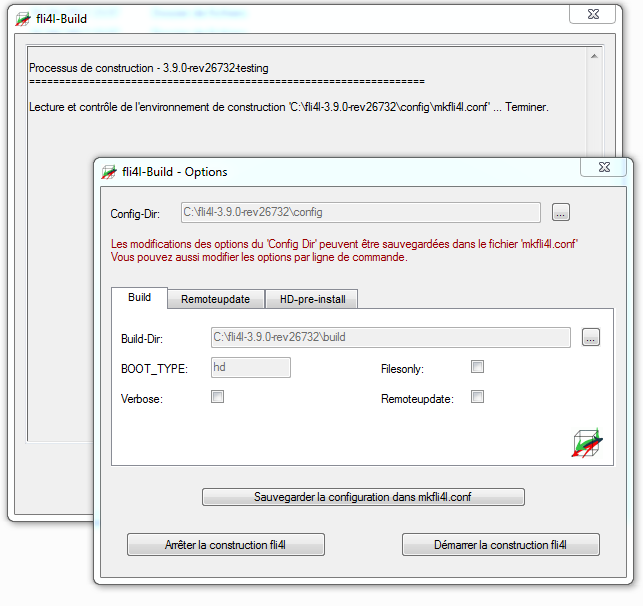
\includegraphics[width=\columnwidth]{win_build_build}
  \caption{Einstellungen}
  \label{fig:win_build_build}
  \end{figure}

  In diesem Dialog werden die Einstellungen für die Archiv/Bootmedienerstellung
  festgelegt:
  \begin{itemize}
    \item Build-Dir~-- Verzeichnis für die Archive/CD-Images/...
    \item \var{BOOT\_TYPE}~-- Anzeige des verwendeten/eingestellen \var{BOOT\_TYPE}~-- nicht änderbar
    \item Verbose~-- Aktivierung von zusätzlichen Ausgaben während der Erstellung
    \item Filesonly~-- es werden nur die Archive erstellt~-- kein bootmedium/kein Image
    \item Remoteupdate~-- Aktivierung des Remoteupdates per SCP
  \end{itemize}

  Mit der Schaltfläche \textbf{Aktuelle Einstellungen in mkfli4l.txt speichern}
  können die aktuell eingestellten Werte in der mkfli4l.txt gespeichert werden.

  \subsection{Konfigurationsdialog~-- Einstellungen für Remoteupdate}
  \begin{figure}[ht!]
  \centering
  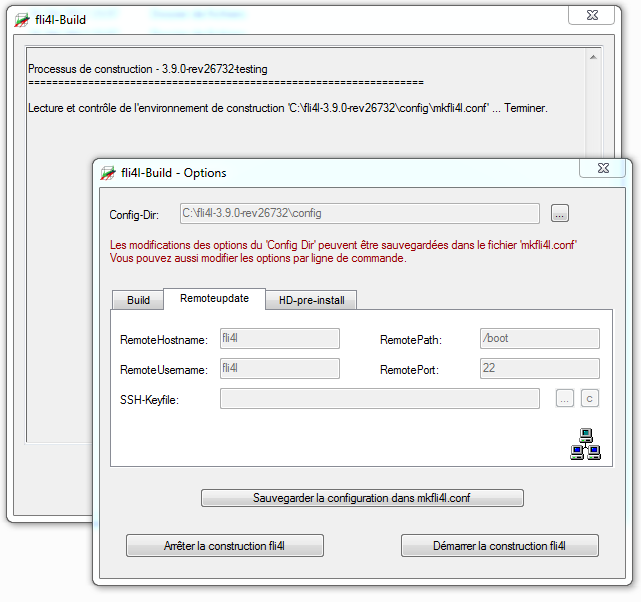
\includegraphics[width=\columnwidth]{win_build_remoteupdate}
  \caption{Einstellungen für Remoteupdate}
  \label{fig:win_build_remoteupdate}
  \end{figure}

  In diesem Dialog werden die Einstellungen für den Remoteupdate festgelegt:
  \begin{itemize}
    \item IP-Adresse oder Hostname
    \item Benutzername auf dem Remote-Host
    \item Remote-Pfad (default: /boot)
    \item Remote-Port (default: 22)
    \item zu verwendendes SSH-Keyfile (ppk-Format von Putty)
  \end{itemize}

  \subsection{Konfigurationsdialog~-- Einstellungen für HD-pre-install}
  \begin{figure}[ht!]
  \centering
  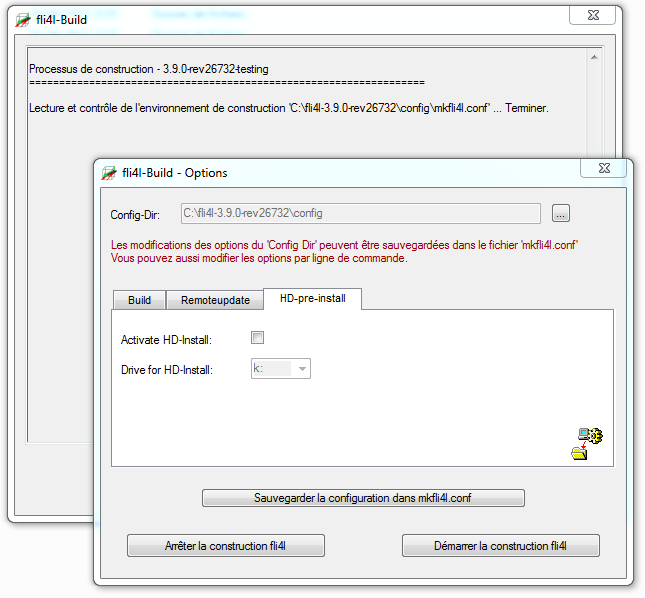
\includegraphics[width=\columnwidth]{win_build_hd_install}
  \caption{Einstellungen für HD-pre-install}
  \label{fig:win_build_hd_install}
  \end{figure}

   In diesem Dialog können die Optionen für den HD-pre-install auf einer
   entsprechend partitionierten und formatierten CompactFlash-Karte
   in einem USB-Reader eingestellt werden.

   Mögliche Optionen:
   \begin{itemize}
     \item HD-pre-install aktivieren
     \item Laufwerksbuchstabe der CF-Karte
  \end{itemize}

  Hinweis zur Partionierung und Formatierung der CF:
  Für eine HD-Installation nach TYP A (siehe dazu Paket HD) muss auf der CF eine
  primäre aktive und formatierte FAT-Partition vorhanden sein. Möchte man
  weiterhin auch eine Datenpartiton benutzen, wird zusätzlich eine Linux-Partition,
  die mit dem Dateisystem ext3 formatiert ist, sowie die Datei \texttt{hd.cfg} auf der
  FAT-Partiton benötigt (hierzu sollten unbedingt die Hinweise im Paket HD beachtet
  werden).

\marklabel{sec:mkfli4lconf}{
  \section{Steuerungsdatei mkfli4l.txt}}
  Seit fli4l-Version 2.1.9 existiert die Steuerungsdatei
  \texttt{$<$config$>$/mkfli4l.txt}. Durch sie werden z.B. vom Standard
  abweichende Verzeichnisse übergeben. Die Steuerungsdatei hat einen
  ähnlichen Aufbau wie die normalen fli4l Konfigurationsdateien.
  Alle Konfigurationsvariablen sind hier optional, d.h. sie müssen nicht
  in der Konfigurationsdatei vorkommen oder können als Kommentar gekennzeichnet
  werden.
  \begin{description}

  \config {BUILDDIR}{BUILDDIR}{BUILDDIR}

  Standardwert: `build'

  Legt fest, in welchem Verzeichnis die fli4l Dateien erzeugt werden sollen.
  Ist die Variable undefiniert, setzt mkfli4l unter Windows `build' relativ zum fli4l
  Wurzelverzeichnis ein und meint damit also das Verzeichnis
  \texttt{build} im fli4l Wurzelverzeichnis:
  \begin{verbatim}
    Pfad/fli4l-x.y.z/build
  \end{verbatim}
  \vspace{-2ex}
  Unter *nix setzt mkfli4l \texttt{$<$config$>$/build} ein und legt damit die
  generierten Dateien zusammen mit der Konfiguration ab.

  Die konfigurierten Pfade in \var{BUILDDIR} müssen der jeweiligen Logik von
  Windows oder *unix entsprechen. Werden relative Pfade gesetzt, wird der Pfad
  durch den Buildprozess passend zu Windows oder *unix konvertiert.

  \config {VERBOSE}{VERBOSE}{VERBOSE}

  Standardwert: \var{VERBOSE='no'}

  Mögliche Werte sind \var{'yes'} oder \var{'no'}. Steuert die \emph{Geschwätzigkeit}
  des Build Prozesses.

  \config {FILESONLY}{FILESONLY}{FILESONLY}

  Standardwert: \var{FILESONLY='no'}

  Mögliche Werte \var{'yes'} oder \var{'no'}. Hiermit kann das Erstellen eines
  Boot-Mediums abgeschaltet werden, es werden also nur die Dateien erzeugt~--

  \config {REMOTEUPDATE}{REMOTEUPDATE}{REMOTEUPDATE}

  Standardwert: \var{REMOTEUPDATE='no'}

  Mögliche Werte \var{'yes'} oder \var{'no'}. Aktiviert das automatische
  Übertragen der erstellten Dateien mittels SCP auf den Router. Dieses setzt
  ein installiertes Paket \jump{OPTSSHD}{SSHD} mit aktiviertem \texttt{scp}
  voraus.  Siehe dazu auch die folgenden Variablen.

  \config {REMOTEHOSTNAME}{REMOTEHOSTNAME}{REMOTEHOSTNAME}

  Standardwert: \var{REMOTEHOSTNAME=''}

  Gibt den Ziel-Hostnamen für den SCP Datentransfer an.
  Sollte kein Name angegeben sein, wird dieser der Variable
  \jump{HOSTNAME}{\var{HOSTNAME}} entnommen.

  \config {REMOTEUSERNAME}{REMOTEUSERNAME}{REMOTEUSERNAME}

  Standardwert: \var{REMOTEUSERNAME='fli4l'}

  Username für den SCP Datentransfer.

  \config {REMOTEPATHNAME}{REMOTEPATHNAME}{REMOTEPATHNAME}

  Standardwert: \var{REMOTEPATHNAME='/boot'}

  Ziel-Pfad für den SCP Datentransfer.

  \config {REMOTEPORT}{REMOTEPORT}{REMOTEPORT}

  Standardwert: \var{REMOTEPORT='22'}

  Zielport für den SCP Datentransfer.

  \config {SSHKEYFILE}{SSHKEYFILE}{SSHKEYFILE}

  Standardwert: \var{SSHKEYFILE=''}

  Hier kann man eine SSH-Keydatei für den SCP-Remoteupdate angeben.
  Es kann somit ein Update ohne Angabe eines Passwortes erfolgen.
  
  \config {REMOTEREMOUNT}{REMOTEREMOUNT}{REMOTEREMOUNT}
  
  Standardwert: \var{REMOTEREMOUNT='no'}
  
  Mögliche Werte \var{'yes'} oder \var{'no'}. Wird hier \var{'yes'}
  gesetzt, wird ein eventuell Readonly eingehängtes Bootdevice "/boot"
  für das Remoteupdate Readwrite gemountet um das Remoteupdate möglich
  zu machen. 

  \config {TFTPBOOTPATH}{TFTPBOOTPATH}{TFTPBOOTPATH}

  Pfad an dem das Netboot-Image abgelegt wird.

  \config {TFTPBOOTIMAGE}{TFTPBOOTIMAGE}{TFTPBOOTIMAGE}

  Name des Netboot-Images.

  \config {PXESUBDIR}{PXESUBDIR}{PXESUBDIR}

  Unterverzeichnis für die PXE-Dateien relativ zu TFTPBOOTPATH.


  \config {SQUEEZE\_SCRIPTS}{SQUEEZE\_SCRIPTS}{SQUEEZESCRIPTS}

   Aktiviert bzw. deaktiviert das Squeezen (Kommprimieren) von
   Skripten.
   Das Komprimieren eines Skripts mit Squeeze entfernt alle Kommentare und
   Zeileneinrückungen.
   Im Normalfall sollte hier immer der Standardwert \var{'yes'} benutzt werden.

  \config {MKFLI4L\_DEBUG\_OPTION}{MKFLI4L\_DEBUG\_OPTION}{MKFLI4LDEBUGOPTION}

   Es können zum Debuggen zusätzliche Optionen an das \jump{mkfli4l}{mkfli4l-Programm} übergeben
   werden.

  \end{description}

  \chapter{Anbindung von PCs im LAN}

  Für jeden Rechner im LAN ist einzustellen:

  \begin{enumerate}
  \item IP-Adresse (siehe \smalljump{sec:pc-lan-ip}{IP-Adresse})
  \item Name des Rechners plus Wunsch-Domain-Name
    (siehe \smalljump{sec:pc-lan-name}{Rechnername und Domain})
  \item Standard-Gateway (siehe \smalljump{sec:pc-lan-gateway}{Gateway})
  \item IP-Adresse des DNS-Servers (siehe \smalljump{sec:pc-lan-dns}{DNS-Server})
  \end{enumerate}

  \marklabel{sec:pc-lan-ip}{\section{IP-Adresse}}
  Die IP-Adresse muss im gleichen Netz wie die IP-Adresse des
  fli4l-Routers (auf Ethernet-Seite) liegen, also z.B. 192.168.6.2,
  wenn der fli4l die Adresse 192.168.6.1 hat.
  Kein Rechner darf die gleiche IP-Adresse haben, weshalb man am
  besten (nur) die letzte Zahl ändert. Auch ist darauf zu achten, dass
  man hier die gleiche IP-Adresse angibt, wie man es für diesen
  Rechner in der Datei config/base.txt angegeben hat.

  \marklabel{sec:pc-lan-name}{\section{Rechnername und Domain}}
  Der Name des Rechners ist dann z.B. ``mein-pc'', die Domain ``lan.fli4l''.

  \wichtig{Die im PC eingestellte Domain muss identisch mit der
  gewählten Domain im fli4l-Rechner sein, wenn man den fli4l-Router
  als DNS-Server verwenden will. Sonst kann es im Netz erhebliche
  Probleme geben.}

  Grund: Windows-Rechner suchen regelmäßig nach Rechnern mit dem Namen
  ihrer Arbeitsgruppte: WORKGROUP.meine-domain.fli4l. Ist dies nicht die in fli4l
  eingestellte Domain (hier: meine-domain.fli4l), wird fli4l
  versuchen, diese Anfrage durch Weiterleiten ins Internet zu
  beantworten \ldots

  Einzutragen ist die Domain in den TCP/IP Einstellungen des Rechners.

  \subsection{Windows 2000}

  Für Windows 2000 findet man das unter:

  \noindent Start \pfeil\\
  \hspace*{2ex}Einstellungen \pfeil\\
  \hspace*{4ex}Systemsteuerung \pfeil\\
  \hspace*{6ex}Netzwerk- und DFÜ-Verbindungen \pfeil\\
  \hspace*{8ex}LAN-Verbindung \pfeil\\
  \hspace*{10ex}Eigenschaften \pfeil\\
  \hspace*{12ex}Internetprotokoll (TCP/IP) \pfeil\\
  \hspace*{14ex}Eigenschaften \pfeil\\
  \hspace*{16ex}Erweitert\ldots \pfeil\\
  \hspace*{18ex}DNS \pfeil\\
  \hspace*{20ex}DNS-Suffix hinzufügen \pfeil\\

  ``lan.fli4l'' (bzw. die eingestellte domain) eingeben (ohne ``''!)
  \pfeil OK drücken.

\subsection{NT 4.0}

  Start \pfeil\\
  \hspace*{2ex}Einstellungen \pfeil\\
  \hspace*{4ex}Systemsteuerung  \pfeil\\
  \hspace*{6ex}Netzwerk \pfeil\\
  \hspace*{8ex}Protokolle \pfeil\\
  \hspace*{10ex}TCP/IP \pfeil\\
  \hspace*{12ex}Eigenschaften \pfeil\\
  \hspace*{14ex}DNS \pfeil\\
  \hspace{16ex}\begin{itemize}
  \item Hostname eintragen (eigener Rechnername)
  \item Domäne eintragen (wie in config/base.txt)
  \item IP-Adresse vom fli4l-Router hinzufügen
  \item DNS-Suffix hinzufügen (Domäne hinzufügen~-- siehe
    2 Zeilen höher)
  \end{itemize}

\subsection{Win95/98}

  Start \pfeil\\
  \hspace*{2ex}Einstellungen \pfeil\\
  \hspace*{4ex}Systemsteuerung \pfeil\\
  \hspace*{6ex}Netzwerk \pfeil\\
  \hspace*{8ex}Konfiguration \pfeil\\
  \hspace*{10ex}TCP/IP (jenes, das an die Netzwerkkarte zum Router\\
  \hspace*{10ex}angebunden ist) \pfeil\\
  \hspace*{12ex}Eigenschaften \pfeil\\
  \hspace*{14ex}DNS-Konfiguration:

  DNS aktivieren und bei ``Domäne:'' dann ``lan.fli4l'' eingeben (ohne ``''!).

\subsection{Windows XP}

  Für Windows XP findet man das unter:

  \noindent Start \pfeil\\
  \hspace*{2ex}Einstellungen \pfeil\\
  \hspace*{4ex}Systemsteuerung \pfeil\\
  \hspace*{6ex}Netzwerkverbindungen \pfeil\\
  \hspace*{8ex}LAN-Verbindung \pfeil\\
  \hspace*{10ex}Eigenschaften \pfeil\\
  \hspace*{12ex}Internetprotokoll (TCP/IP) \pfeil\\
  \hspace*{14ex}Eigenschaften \pfeil\\
  \hspace*{16ex}Erweitert\ldots \pfeil\\
  \hspace*{18ex}DNS \pfeil\\
  \hspace*{20ex}DNS-Suffix für diese Verbindung \pfeil\\

  ``lan.fli4l'' (bzw. die eingestellte domain) eingeben (ohne ``''!)
  \pfeil OK drücken.

\subsection{Windows 7}

  Für Windows 7 findet man das unter:

  \noindent Windows Button (ex. Start) \pfeil\\
  \hspace*{2ex}Systemsteuerung \pfeil\\
  \hspace*{4ex}Netzwerk und Internet \pfeil\\
  \hspace*{6ex}Netzwerk- und Freigabecenter \pfeil\\
  \hspace*{8ex}LAN-Verbindung \pfeil\\
  \hspace*{10ex}Eigenschaften \pfeil\\
  \hspace*{12ex}Internetprotokoll Version 4 (TCP/IPv4) \pfeil\\
  \hspace*{14ex}Eigenschaften \pfeil\\
  \hspace*{16ex}Erweitert\ldots \pfeil\\
  \hspace*{18ex}DNS \pfeil\\
  \hspace*{20ex}DNS-Suffix für diese Verbindung \pfeil\\

  ``lan.fli4l'' (bzw. die eingestellte domain) eingeben (ohne ``''!)
  \pfeil OK drücken.

\subsection{Windows 8}

  Für Windows 8 findet man das unter:

  \noindent Gleichzeitig Windows- und X-Taste drücken \pfeil\\
  \hspace*{2ex}Systemsteuerung \pfeil\\
  \hspace*{4ex}Netzwerk und Internet \pfeil\\
  \hspace*{6ex}Netzwerk- und Freigabecenter \pfeil\\
  \hspace*{8ex}Ihr Netzwerk wählen (Ehternet oder WLAN) \pfeil\\
  \hspace*{10ex}Eigenschaften \pfeil\\
  \hspace*{12ex}Internetprotokoll Version 4 (TCP/IPv4) \pfeil\\
  \hspace*{14ex}Eigenschaften \pfeil\\
  \hspace*{16ex}Erweitert\ldots \pfeil\\
  \hspace*{18ex}DNS \pfeil\\
  \hspace*{20ex}DNS-Suffix für diese Verbindung \pfeil\\

  ``lan.fli4l'' (bzw. die eingestellte domain) eingeben (ohne ``''!)
  \pfeil OK drücken.

  \marklabel{sec:pc-lan-gateway}{\section{Gateway}}
  Die Angabe des Standard-Gateways ist unbedingt erforderlich, denn
  ohne die Angabe der richtigen IP-Adresse an dieser Stelle
  funktioniert nichts.  Es muß hier die IP-Adresse des fli4l-Routers
  (auf Ethernet-Seite) angegeben werden, also z.B. 192.168.6.4
  entsprechend der IP-Adresse, die hier in der Datei config/base.txt
  für den fli4l-Router angegeben wurde.

  Es ist falsch, den fli4l-Router als Proxy in der Windows- oder
  Browser- Konfiguration einzutragen~-- außer man setzt ein Proxy auf
  dem fli4l-Router ein. Im Normalfall ist fli4l kein Proxy, daher
  bitte \emph{nicht} fli4l als Proxy angeben!

\marklabel{sec:pc-lan-dns}{\section{DNS-Server}}

  Als IP-Adresse des DNS-Servers gibt man nicht die Adresse des
  Provider-DNS-Servers an, sondern die des fli4l-Routers (Ethernet),
  da dieser nun selbst Anfragen beantworten kann bzw. diese bei
  Unkenntnis ins Internet weiterleitet.

  Mit der Konstruktion von fli4l als DNS-Server werden viele von den
  Windows-PCs ausgeführten Anfragen nicht ins Internet weitergeroutet,
  sondern werden direkt vom fli4l-Router beantwortet.

\marklabel{sec:pc-lan-misc}{\section{Verschiedenes}}

  Die Punkte 1 bis 4 brauchen bei konfiguriertem DHCP-Server nicht
  eingetragen zu werden, da dann der fli4l-Router die notwendigen Daten
  automatisch übermittelt.

  \textbf{Internetoptionen:} Bei Verbindungen muß ``keine Verbindung wählen'' ausgewählt sein.
  Bei Einstellungen für lokales Netzwerk(LAN): es darf hier NICHTS
  angegeben werden (es sei dann es wird \var{OPT\_\-P}roxy verwendet).
  Beides sind Standardeinstellungen, die im Normalfall nicht geändert
  werden müssen.

\marklabel{IMONDSCHNITTSTELLE}{
    \chapter{Client-/Server-Schnittstelle imon}
  }

  \marklabel{sec:imond}{
    \section{imon-Server imond}}

  imond ist ein netzwerkfähiges Server-Programm, welches bestimmte
  Anfragen beantwortet oder auch Kommandos zur Steuerung des Routers
  entgegennehmen kann.

  Ausserdem steuert imond das Least-Cost-Routing. Dazu verwendet er
  eine Konfigurationsdatei /etc/imond.conf, welche beim Booten
  automatisch aus den \var{ISDN\_\-CIRC\_\-x\_\-XXX}-Variablen der Datei
  config/isdn.txt und anderen über ein Shell-Script erzeugt wird.

  imond läuft permanent als Daemon und horcht gleichzeitig auf
  TCP/IP-Port 5000 und Device /dev/isdninfo.

  Folgende Kommandos sind über den TCP/IP-Port 5000 möglich:
  \begin{table}
    \textbf{Admin-Befehle}

    \vspace{1ex}
    \begin{tabular}{lp{9cm}}

      addlink ci-index              & Channel zum Circuit hinzufügen
                                      (Channel-Bundling) \\
      adjust-time seconds           & Ändert die Uhrzeit des Routers um die
                                      angegebenen Sekunden \\
      delete filename pw            & Löscht die Datei auf dem Router \\
      hup-timeout \#ci-index [value]& Anzeigen bzw. Setzen des HUP-Timeout für
                                      ISDN-Circuits \\
      removelink ci-index           & Zusätzlichen Channel wieder entfernen \\
      reset-telmond-log-file        & Löschen der telmond-Protokolldatei \\
      reset-imond-log-file          & Löschen der imond-Protokolldatei \\
      receive filename \#bytes pw   & Eine Datei auf den Router übertragen.
                                      Dazu quittiert imond den Befehl mit
                                      einem ACK (0x06). Danach wird die Datei
                                      in 1024er-Blöcken übertragen, die imond
                                      auch jeweils mit einem ACK bestätigt.
                                      Als letztes übermittelt imond noch ein
                                      OK. \\
      send filename pw              & Wenn das Passwort stimmt und die Datei
                                      existiert, liefert imond ein OK \#bytes.
                                      Anschliessend überträgt imond die Datei
                                      in 1024er Blöcken, die jeweils mit
                                      einem ACK (0x06) bestätigt werden
                                      müssen. Als letztes liefert imond noch
                                      ein OK. \\
      support pw                    & Liefert den Status/Konfiguration vom
                                      Router \\
      sync                          & Synchronisiert den Cache von gemounteten
                                      Laufwerken \\
    \end{tabular}
  \end{table}


  \begin{table}
    \textbf{Admin- oder User-Befehle}

    \vspace{1ex}
    \begin{tabular}{lp{9cm}}

      dial                      &    Wählt den Provider an
                                     (Default-Route-Circuit) \\
      dialmode [auto|manual|off]&    Liefert bzw. setzt den Dialmode \\
      disable                   &    Hängt ein und setzt dialmode auf ``off''
                                      \\
      enable                    &    Setzt dialmode auf ``auto'' \\
      halt                      &    Fährt den Router sauber herunter \\
      hangup [\#channel-id]     &    Hängt ein \\
      poweroff                  &    Fährt den Router herunter und schaltet ab \\
      reboot                    &    Reboot vom i4l-Router! \\
      route [ci-index]          &    Setzen Default-Route auf Circuit X
                                     (0=automatisch) \\
    \end{tabular}
  \end{table}


  \begin{table}
    \textbf{User-Befehle}

    \vspace{1ex}
    \begin{tabular}{lp{9cm}}
      channels                  & Ausgabe Anzahl der verfügbaren ISDN-Kanäle\\
      charge \#channel-id       & Ausgabe der Online-Kosten für einen
                                  Channel\\
      chargetime \#channel-id   & Online-Zeit unter Berücksichtigung des
                                  Taktes\\
      circuit [ci-index]        & Ausgabe eines Circuit-Namens\\
      circuits                  & Ausgabe Anzahl der Default-Route-Circuits\\
      cpu                       & Liefert die Auslastung der CPU in Prozent\\
      date                      & Ausgabe Datum/Uhrzeit\\
      device ci-index           & Liefert das Device des Circuits\\
      driverid \#channel-id     & Ausgabe Driver-Id für Channel X\\
      help                      & Ausgabe Hilfe\\
      inout \#channel-id        & Ausgabe der Richtung (incoming/outgoing)\\
      imond-log-file            & Ausgabe imond-Protokolldatei\\
      ip \#channel-id           & Ausgabe der IP\\
      is-allowed command        & Ausgabe, ob Befehl konfiguriert/gültig
                                  ist\newline
                                  Mögliche Befehle:
                                    dial|dialmode|route|reboot|
                                    imond-log|telmond-log|mgetty-log \\
      is-enabled                & Ausgabe, ob dialmode auf off (0) oder auto
                                  (1)\\
      links ci-index            & Ausgabe Anzahl momentaner Channel 0, 1 oder
                                  2, 0 heisst: Kein Channel-Bundling möglich\\
      log-dir imond|telmond|mgetty& Liefert das Logverzeichnis\\
      mgetty-log-file           & Ausgabe mgetty-Protokolldatei\\
      online-time \#channel-id  & Ausgabe Online-Zeit der akt. Verbindung in
                                  hh:mm:ss\\
      pass [password]           & Abfrage, ob Password nötig bzw. Password-
                                  Eingabe\newline
                                  1 Userpassword gesetzt\newline
                                  2 Adminpassword gesetzt\newline
                                  4 imond befindet sich im Admin-Modus\\
      phone \#channel-id        & Ausgabe Telefonnummer/Name des ``Gegners''\\
      pppoe                     & Liefert die Anzahl der pppoe-Devices (also 0
                                  oder 1)\\
      quantity \#channel-id     & Liefert die übertragenen Datenmengen (in
                                  Byte)\\
      quit                      & Beenden der Verbindung zu imond\\
      rate \#channel-id         & Ausgabe Übertragungsraten (incoming/outgoing
                                  in B/sec)\\
      status \#channel-id       & Ausgabe Status für Channel X\\
      telmond-log-file          & Ausgabe telmond-Protokolldatei\\
      time \#channel-id         & Ausgabe Summe Online-Zeiten, Format
                                  hh:mm:ss\\
      timetable [ci-index]      & Ausgabe der Zeittabelle für LC-Routing\\
      uptime                    & Ausgabe der Uptime des Routers in Sekunden\\
      usage \#channel-id        & Ausgabe Art der Verbindung, mögliche
                                  Antworten: Fax, Voice, Net, Modem, Raw\\
      version                   & Ausgabe der Protokoll- und
                                  Programm-Version\\
    \end{tabular}
  \end{table}


  Der TCP/IP-Port 5000 ist nur vom maskierten LAN aus erreichbar.
  Standardmäßig wird ein Zugriff von aussen über die
  Firewall-Konfiguration abgeblockt.

  Imond unterstützt zwei Benutzerebenen: den User- und den
  Admin-Modus.  Für beide Ebenen kann ein Passwort gesetzt werden
  mittels \var{IMOND\_\-PASS} bzw.  \var{IMOND\_ADMIN\_\-PASS}. Dadurch
  werden die imon-Clients von imond gezwungen, eine Password-Abfrage
  durchzuführen und anschließend das Password an imond zu übertragen.
  Solange dieses Password nicht übermittelt wurde, nimmt imond nur die
  beiden Kommandos ``pass'' und ``quit'' entgegen. Alle anderen werden
  mit einem Fehler zurückgewiesen.

  Möchte man das weiter einschränken, z.B. den Zugriff nur von nur
  einem PC erlauben, muss die Firewall-Konfiguration angepasst werden.

  Die Befehle

\begin{example}
\begin{verbatim}
         enable/disable/dialmode   dial/hangup   route   reboot/halt
\end{verbatim}
\end{example}

  können durch die Konfigurationsvariablen \var{IMOND\_\-XXX} global ein- oder
  abgeschaltet werden (s. Kapitel ``Konfiguration'').

  Mit einem Unix/Linux-Rechner (oder einem Windows-Rechner in der DOS-Box)
  kann man das Ganze leicht ausprobieren:

  Nach Eingabe von

\begin{example}
\begin{verbatim}
        telnet fli4l 5000        \# oder entsprechender Name des fli4l-Routers
\end{verbatim}
\end{example}

  kann man direkt die oben aufgeführten Kommandos eingeben und sich
  die Ausgabe anschauen.

  Zum Beispiel bekommt man mit ``help'' die Hilfe angezeigt, mit
  ``quit'' wird die Verbindung zum imond abgebaut.

\marklabel{sec:leastcostrouting}{
  \subsection{Least-Cost-Routing~-- Funktionsweise}
  }

  imond konstruiert aus der Konfigurationsdatei /etc/imond.conf
  (welche wiederum beim Booten aus den Konfigurationsvariablen
  \var{ISDN\_\-CIRC\_\-x\_\-TIMES} usw.  erstellt wird), eine zeitabhängige
  Tabelle (Time-Table). Diese umfasst eine komplette Kalenderwoche im
  1-Stunden-Raster (168 Stunden = 168 Bytes). Die Tabelle setzt sich
  jedoch lediglich aus Circuits zusammen, für die eine Default-Route
  definert ist.

  Mit dem imond-Kommando ``timetable'' kann man sich diese Tabelle
  anschauen.

  Hier ein Beispiel:

  Nehmen wir an, dass 3 Circuits definiert wurden, nämlich:

\begin{example}
\begin{verbatim}
        CIRCUIT_1_NAME='Addcom'
        CIRCUIT_2_NAME='AOL'
        CIRCUIT_3_NAME='Firma'
\end{verbatim}
\end{example}

  wobei lediglich die ersten beiden Circuits mit Default-Routen belegt
  sind, also die enstprechenden Variablen ISDN\_CIRC\_x\_ROUTE den
  Wert `0.0.0.0' haben.

  Wenn die dazugehörigen Variablen \var{ISDN\_\-CIRC\_\-x\_\-TIMES} folgendermaßen
  aussehen:

\begin{example}
\begin{verbatim}
        ISDN_CIRC_1_TIMES='Mo-Fr:09-18:0.0388:N Mo-Fr:18-09:0.0248:Y
                      Sa-Su:00-24:0.0248:Y'

        ISDN_CIRC_2_TIMES='Mo-Fr:09-18:0.019:Y Mo-Fr:18-09:0.049:N
                      Sa-Su:09-18:0.019:N Sa-Su:18-09:0.049:N'

        ISDN_CIRC_3_TIMES='Mo-Fr:09-18:0.08:N Mo-Fr:18-09:0.03:N
                      Sa-Su:00-24:0.03:N'
\end{verbatim}
\end{example}

  dann wird daraus folgende Datei /etc/imond.conf:

\begin{example}
\begin{verbatim}
        #day  hour  device  defroute  phone        name        charge  ch-int
        Mo-Fr 09-18 ippp0   no        010280192306 Addcom      0.0388   60
        Mo-Fr 18-09 ippp0   yes       010280192306 Addcom      0.0248   60
        Sa-Su 00-24 ippp0   yes       010280192306 Addcom      0.0248   60
        Mo-Fr 09-18 ippp1   yes       019160       AOL  0.019   180
        Mo-Fr 18-09 ippp1   no        019160       AOL  0.049   180
        Sa-Su 09-18 ippp1   no        019160       AOL  0.019   180
        Sa-Su 18-09 ippp1   no        019160       AOL  0.049   180
        Mo-Fr 09-18 isdn2   no        0221xxxxxxx  Firma       0.08     90
        Mo-Fr 18-09 isdn2   no        0221xxxxxxx  Firma       0.03     90
        Sa-Su 00-24 isdn2   no        0221xxxxxxx  Firma       0.03     90
\end{verbatim}
\end{example}

  imond erstellt dann im Speicher folgende Time-Table~-- hier die Ausgabe
  über das imond-Kommando ``timetable'':

\begin{example}
\begin{verbatim}
         0  1  2  3  4  5  6  7  8  9 10 11 12 13 14 15 16 17 18 19 20 21 22 23
     --------------------------------------------------------------------------
     Su  3  3  3  3  3  3  3  3  3  3  3  3  3  3  3  3  3  3  3  3  3  3  3  3
     Mo  2  2  2  2  2  2  2  2  2  4  4  4  4  4  4  4  4  4  2  2  2  2  2  2
     Tu  2  2  2  2  2  2  2  2  2  4  4  4  4  4  4  4  4  4  2  2  2  2  2  2
     We  2  2  2  2  2  2  2  2  2  4  4  4  4  4  4  4  4  4  2  2  2  2  2  2
     Th  2  2  2  2  2  2  2  2  2  4  4  4  4  4  4  4  4  4  2  2  2  2  2  2
     Fr  2  2  2  2  2  2  2  2  2  4  4  4  4  4  4  4  4  4  2  2  2  2  2  2
     Sa  3  3  3  3  3  3  3  3  3  3  3  3  3  3  3  3  3  3  3  3  3  3  3  3

     No.  Name                   DefRoute  Device  Ch/Min   ChInt
      1   Addcom                   no      ippp0   0.0388     60
      2   Addcom                   yes     ippp0   0.0248     60
      3   Addcom                   yes     ippp0   0.0248     60
      4   AOL               yes     ippp1   0.0190    180
      5   AOL               no      ippp1   0.0490    180
      6   AOL               no      ippp1   0.0190    180
      7   AOL               no      ippp1   0.0490    180
      8   Firma                    no      isdn2   0.0800     90
      9   Firma                    no      isdn2   0.0300     90
     10   Firma                    no      isdn2   0.0300     90
\end{verbatim}
\end{example}

  Für den Circuit 1 (Addcom) sind also drei Zeitbereiche (1-3)
  eingetragen, für Circuit 2 (AOL) vier Zeitbereiche (4-7) und
  für den letzen drei Zeitbereiche (8-10).

  In der Time-Table werden jeweils die Indices ausgegeben, welche für
  die jeweilige Stunde gültig sind. Hier tauchen lediglich die Indices
  2-4 auf, da alle anderen keine LC-Default-Routen sind.

  Sieht man in der Tabelle irgendwo Nullen, gibt es Lücken in den
  \var{ISDN\_\-CIRC\_\-X\_\-TIMES}-Werten. Dann existiert zu diesen Zeiten keine
  Default-Route, Internet-Zugang abgeknipst!

  Beim Programmstart ermittelt imond zunächst den Wochentag und die
  aktuelle Stunde. Anschließend wird dann über die Time-Table der
  Index ermittelt und damit dann auch der entsprechende Circuit. Auf
  diesen wird dann die Default-Route gesetzt.

  Bei Zustandsänderungen der Channels, z.B. Wechsel von online
  nach offline~-- jedoch spätestens nach 1 Minute~-- geht das Spiel von
  neuem los: Zeit ermitteln, Lookup in Tabelle, Default-Route-Circuit
  ermitteln.

  Ändert sich der aktuell verwendete Circuit, z.B. montags um 18:00
  Uhr, wird die alte Default-Route gelöscht, eine vielleicht
  bestehende Verbindung beendet (sorry\ldots) und anschließend die
  Default-Route auf den neuen Circuit gesetzt. Dies kann von imond bis
  zu 60 Sekunden später bemerkt werden, also wird spätestens um
  18:00:59 umgeschaltet.

  Bei Circuits, die keine Default-Route belegen, ändert sich überhaupt
  nichts. Hier wird der Inhalt von \var{ISDN\_\-CIRC\_\-x\_\-TIMES} lediglich zur
  Berechnung der Telefonkosten verwendet. Diese können dann relevant
  sein, wenn man über den Client imonc das LC-Routing temporär
  ausschaltet und einen Circuit manuell wählt.

  Man kann sich jedoch auch die Tabellen für andere
  Zeitbereich-Indices (im Beispiel von 1 bis 10) anschauen, auch die
  der ``Non-LC-Default-Route-Circuits''.

  Kommando:

\begin{example}
\begin{verbatim}
                    timetable index
\end{verbatim}
\end{example}

  Beispiel:

\begin{example}
\begin{verbatim}
                    telnet fli4l 5000
                    timetable 5
                    quit
\end{verbatim}
\end{example}

  Die Ausgabe sieht dann so aus:

\begin{example}
\begin{verbatim}
         0  1  2  3  4  5  6  7  8  9 10 11 12 13 14 15 16 17 18 19 20 21 22 23
     --------------------------------------------------------------------------
     Su  0  0  0  0  0  0  0  0  0  0  0  0  0  0  0  0  0  0  0  0  0  0  0  0
     Mo  5  5  5  5  5  5  5  5  5  0  0  0  0  0  0  0  0  0  5  5  5  5  5  5
     Tu  5  5  5  5  5  5  5  5  5  0  0  0  0  0  0  0  0  0  5  5  5  5  5  5
     We  5  5  5  5  5  5  5  5  5  0  0  0  0  0  0  0  0  0  5  5  5  5  5  5
     Th  5  5  5  5  5  5  5  5  5  0  0  0  0  0  0  0  0  0  5  5  5  5  5  5
     Fr  5  5  5  5  5  5  5  5  5  0  0  0  0  0  0  0  0  0  5  5  5  5  5  5
     Sa  0  0  0  0  0  0  0  0  0  0  0  0  0  0  0  0  0  0  0  0  0  0  0  0

     No.  Name                   DefRoute  Device  Ch/Min   ChInt
      5   AOL               no      ippp1   0.0490    180
\end{verbatim}
\end{example}

  Alles klar?

  Mit dem imond-Kommando ``route'' kann das LC-Routing ein- und
  ausgeschaltet werden. Bei Angabe eines positiven Circuit-Indices
  (1\ldots N) wird die Default-Route auf den angegebenen Circuit
  gelegt. Ist der Index 0, wird das LC-Routing wieder aktiviert und
  der Circuit automatisch ausgewählt.


  \subsection{Zur Berechnung der Onlinekosten}

  Das ganze Modell zur Berechnung der Onlinekosten funktioniert nur
  korrekt, wenn der Zeittakt für einen Circuit (Variable
  \var{ISDN\_\-CIRC\_\-x\_\-CHARGEINT}) über die ganze Woche konstant ist. Dies
  ist im Normalfall bei Internet-Providern die Regel. Wählt man sich
  jedoch über die Telekom (ich meine nicht T-Online!) z.B. in sein
  Firmennetz ein, gilt das als ganz normales Telefongespräch. Und da
  wechselt ab 18:00 der Takt von 90 Sekunden auf 4 Minuten (Stand Juni
  00). Deshalb ist die Definition von

\begin{example}
\begin{verbatim}
        ISDN_CIRC_3_CHARGEINT='90'
        ISDN_CIRC_3_TIMES='Mo-Fr:09-18:0.08:N Mo-Fr:18-09:0.03:N Sa-Su:00-24:0.03:N'
\end{verbatim}
\end{example}

  eigentlich nicht ganz korrekt. Es sind zwar abends umgerechnet auf
  die Minute 3 Pfennig (4 Minuten kosten 12 Telekom-Pfennige), jedoch
  ist der Takt falsch. Deshalb können bei der Kostenanzeige
  Differenzen zu den tatsächlichen Zahlen auftreten.

  Hier ist ein Tipp, wie verschieden lange Taktzeiten dennoch richtig
  berücksichtigt werden können (auch wichtig für
  \var{ISDN\_\-CIRC\_\-x\_\-CHARGEINT}): Man definiert einfach 2 Circuits,
  einen für tagsüber mit \var{ISDN\_\-CIRC\_\-1\_\-CHARGEINT}=`90' und den
  anderen mit \var{ISDN\_\-CIRC\_\-2\_\-CHARGEINT}=`240'.
  Natürlich muss man dann auch noch \var{ISDN\_\-CIRC\_\-x\_\-TIMES}
  entsprechend wählen, damit tagsüber Circuit 1 und abends Circuit 2
  verwendet wird.

  Wie gesagt: Bei Nutzung von Verbindungen zu Internet-Providern gibt
  es das Problem nicht, weil dort der Zeittakt immer konstant ist und
  lediglich die Kosten pro Minute wechseln (oder gibt es sowas doch???
  Ich traue T-* alles zu :-).

  % Synchronized to r30003
  \marklabel{sec:winimonc}{
    \section{Windows-Client imonc.exe}}

  \subsection{Introduction}

  imond on the router and on the client imonc as a team have
  two use modes: the user and the admin mode. In admin mode, all
  controls are enabled. In user mode the variables
  \jump{IMONDENABLE}{\var{IMOND\_ENABLE}}, \jump{IMONDDIAL}{\var{IMOND\_DIAL}}, 
  \jump{IMONDROUTE}{\var{IMOND\_ROUTE}} and \jump{IMONDREBOOT}{\var{IMOND\_REBOOT}}
  control if the respective functions are available. If all of these
  variables are set to `no ', this means that all buttons in the overview page
  are disabled except for the exit and the admin mode button. The
  decision whether the user or admin mode is used, is based on the
  transmitted password. By clicking the button admin mode, located in the
  status bar, you may switch to the admin mode at any time by entering the
  admin password. To switch back imonc must be restarted.

  Once imonc is started an additional tray icon is displayed, which
  shows the connection status of existing channels.

  The colors mean:
  \begin{description}
    \item[Red]: Offline
    \item[Yellow]: A connection is in the process of being established
    \item[Light Green]: Online and traffic on the channel
    \item[Dark Green]: Online and (nearly) no traffic on the channel
  \end{description}

  \noindent imonc shows a behavior a little different from the Windows standard
  when clicking on the minimize button in the title bar. This minimizes imonc
  to the system tray only a tray icon near the clock remains. Double clicking
  on the tray icon with the left mouse button brings imonc's window back to
  the foreground. With the right mouse button you may use the context menu,
  of the tray icon to execute the main imonc commands die angezeigten
         without displaying its
  main window.

  Imonc stores many properties (including all columns widths of the string grids)
  in the registry, so its appearance may be widely adapted to your needs. Imonc
  uses the registry key HKCU{\textbackslash}Software{\textbackslash}fli4l
  to store this informations

  If even after careful reading of the documentation problems on imonc or the
  router itself still remain you can post to the newsgroup. It makes sense
  to note the support information you get when choosing SystemInfo and then Info
  on the About page of the imonc client. The router password will be queried
  then (not the imond password) and after that imonc will create a file fli4lsup.txt
  that contains all the important information regarding the router, including
  imonc. This file can be posted on the newsgroup when explicitely demanded
  and will give much better chance for quick help.

  Further details concerning the development of the Windows imonc client can be found
  on the homepage of Windows Imonc \altlink{http://www.imonc.de/}. Here you can
  see what new features and bug fixes will be included in the next version.
  In addition, you will find the latest imonc version, if it is not included
  in the FLI4L distribution already.

  \subsection{Start Parameters}

  Imonc requires the name or IP address of the router fli4l. As the default
  the program attempts to establish a connection with the computer ``fli4l''.
  If this entry is correctly entered in the DNS, this should work out of the box.
  Otherwise you can pass following parameters in the link:

  \begin{itemize}
    \item /Server:The router's IP or hostname (short form: /S:IP or hostname)
    \item /Password:password (short form: /P:password)
    \item /log Option for logging communication betweeen imonc und imond. When
      entered a file imonc.log  will be written each time when imonc exits. It
      contains the complete communication and thus can grow quite large. Please
      use this parameter only in case of problems.
    \item /iport:Portnumber Portnumber imond listens to. Default: 5000
    \item /tport:Portnummer Portnumber telmond listens to. Default: 5001
    \item /rc:''Command'' The command provided here will be transmitted to the
      router without further checking and imonc will exit afterwards. 
      If more than one command should be transmitted at once, they must be devided
      by semicolons. You will have to provide an imond password in addition for
      this to work because no password query will be queried. Possible command
      are documented with imond, see chapter 8.1. In addition to the commands
      there another one exists: timesync. If used imonc will synchronize the
      clock of the client with the router's clock. The command dialtimesync is
      not supported anymore, it is substituted by "dial; timesync".
    \item /d:''fli4l-Directory'' Pass the fli4l-directory as a start parameter.
      May be of interest when using more than one fli4l version.
    \item /wait If the hostname can't be reolved imonc will not exit anymore~--
      start another try by doubleclicking the tray icon.
    \item /nostartcheck Disables checking of imonc already running. Only makes
      sense to monitor several different fli4l routers in a net. When using more
      instances the builtin syslog- and \mbox{E-Mail}-capabilites will be disabled.
  \end{itemize}

  Usage (to be entered in the link):

\begin{example}
\begin{verbatim}
X:\...imonc.exe [/Server:Host] [/Password:Password] [/iport:Portnumber]
            [/log] [/tport:Portnumber] [/rc:"Command"]
\end{verbatim}
\end{example}

  Example with IP address:

\begin{example}
\begin{verbatim}
        C:\wintools\imonc /Server:192.168.6.4
\end{verbatim}
\end{example}

  or with name and password:

\begin{example}
\begin{verbatim}
        C:\wintools\imonc /S:fli4l /P:secret
\end{verbatim}
\end{example}

  or with name and password and router command:

\begin{example}
\begin{verbatim}
        C:\wintools\imonc /S:fli4l /P:secret /rc:"dialmode manual"
\end{verbatim}
\end{example}

  \subsection{Overview}

  The Windows client queries some imond information on the existing
  connections and displays it in its window. In addition to general
  status information such as uptime of the router or the time (both locally
  and on the router), for each existing connection the following informations
  are shown:

  \begin{tabular}{lp{9cm}}
    Status             &Connection establishment/Online/Offline\\
    Name               &Telephone number of the caller or circuit name\\
    Direction          &Indicates if a connection is incoming or outgoing\\
    IP                 &IP, that was assigned to the router\\
    IBytes             &Bytes received\\
    OBytes             &Bytes sent\\
    Online time        &Actual online time\\
    Time               &Sum of all online times\\
    KTime              &Sum of all online times in consideration of charge intervals\\
    Cost               &Computed costs\\
  \end{tabular}

  \medskip

  The data is updated every 2 seconds by default. In the context menu of
  this overview it is possible to copy the assigned IP to the clipboard
  as well as hanging up the channel (for each available channel which is
  online at the moment). This is of interest in case that several different
  connections exist, e.g. one to surf the Internet and another to a private
  net and only one of them should be terminated.

  If the telmond process is active on the router, imonc can show information
  about incoming phone calls (ie calling and called MSN) in addition. The last
  incoming phone call is displayed above the buttons. a log of phone calls received
  can be obtained by viewing the calls page.

  By the six buttons in imonc the following commands can be selected:

  \begin{tabular}{clp{9cm}}
    Button & Caption & Function \\
    1& Connect/Disconnect &   Dial/Hang up\\
    2& Add link/Rem link  &   Bundle channels: yes/no~-- only available in admin mode\\
    3& Reboot             &   Reboot fli4l!\\
    4& PowerOff           & Shut down fli4l and power off afterwards\\
    5& Halt               & Shut down fli4l to power off safe afterwards\\
    6& Exit               & Exit client\\
  \end{tabular}

  \medskip

  \noindent The first five commands can be switched on and off individually in the
  router's configuration file config/base.txt for the user mode. In admin mode all
  are enabled. The dialmode controls the dialing behavior of the router:

  \begin{tabular}{lp{9cm}}
    Auto  & The router will establish connections automatically when getting 
    queries from the local net for the circuit concerned.\\
    Manual & The user himself has to establish connections.\\
    Off   & No connections can be established. The dial button is deactivated.\\
  \end{tabular}

  \medskip

  \noindent Note that fli4l by default will dial out independently. So you never
  actually will have to press the connect button\ldots

  It is also possible to manually switch the default route circuit, setting
  the automatic LCR on and off. In the Windows version of imonc the selection
  list `` default route'' is provided for this. In addition you can configure the
  hangup TimeOut time directly in imonc. use the Config button next to the default
  route for this. All configured circuits of the router are displayed here. The
  value in the column Hup-timeout can be edited directly in the string grid
  for ISDN circuits (not yet working for DSL).

  An overview over LCR can be found on the page admin/Timetable.
  There you'll see what circuit imond selects automatically at which time.

  \subsection{Config-Dialog}

  The configuration is reached using the Config button in the status bar. The window
  is divided into the following areas:

  \begin{itemize}
  \item The Area General:
    \begin{itemize}
    \item Actualization Interval: Set here how often the overview should get actualized.
    \item Synchronize Time on Startup: When starting the client's system time and date 
      will get synchronized with the router's system time. You can execute this manually
      by using the button Synchronize on the Overview-page.
    \item Start Minimized: Program will start minimized to the system tray.
    \item Start with Windows: Specify here if the client should start automatically 
      with system start. Provide necessary start-parameters in the field Parameter.
    \item Fetch News from fli4l.de: Should news from fli4l's homepage be fetched and
      displayed by imonc? Then headlines are shown in the status bar. A new page News
      is displayed to show the complete messages.
    \item Logfile for Connections: The file name here is used to save connection lists
      locally on the imonc's system.
    \item TimeOut for router to answer: How long should we wait for an answer from the
      router before assuming that the connection has failed.
    \item Language: Pick the language for imoncs to use.
    \item Confirm Router Commands: If activated all commands influencing the router
      generally have to be confirmed, i.e. Reboot, Hangup \ldots
    \item Hang up even when traffic: No information should be displayed when the
      connection is closed and there is still traffic on the line.
    \item Automatic Connection to the router: Should we try to reconnect to the router
      in case of lost connections (i.e. when rebooting the router).
    \item Minimize Window To System Tray: Should imonc minimize to system tray instead
      of terminating itself when clicking the Exit button.
    \end{itemize}

  \item Proxy Settings:
    Define a proxy for imonc's http-queries here. It will be used for fetching news.
    \begin{itemize}
    \item Activate Proxy-support for Http-queries: Should we use a proxy 
          \begin{itemize}
            \item Address: Address of the proxy server
            \item Port: Port number of the proxy server (default: 8080)
          \end{itemize}
    \end{itemize}
    
  \item TrayIcon:
  	Set the colors of the tray icon next to the clock to your own needs.
  	In addition you can specify that the actual dialmode will set the background
  	color of the tray icon.

  \item Calls: The position of the call notification window will be saved in the
    registry in order to allow to set a fixed position for the window. Simlpy drag the
    window to the desired position.
    \begin{itemize}
      \item Update: Set here in what way imonc will be informed about new calls. There
	are three possibilities. The first is querying the telmond service on the
	router in regular time intervals. A second is evaluating the syslog messages.
	This variant is preferred to the first~- of course, the imon's syslog client
	has to be enabled. If imonc is used with a routed eisfair system the third
	possibility is to use the Capi2Text package for call signaling.
      \item Delete Leading Zeros (Phone Boxes): Phone boxes often use an additional
	Zero to prefix the caller's number. This option will suppress the digit.
      \item Own Area Code: Save your own area code here. If a call with the same
	area code is received it will get suppressed when displaying.
      \item Telephone Book: Here, the file can be specified, in which the local
        Phone book is saved for resolving of the phone number. If the file does not
        exist, it is created by the program.
      \item Logfile: The file name you can specify here is used to save the call
	list locally on the computer. This menu item is only visible if the config
	variable \var{TELMOND\_\-LOG} is set to `yes' (this also applies to the
        call list).
      \item Use External Search: In this area, a program may be specified that will
	be called when a phone number can not be resolved using the local phone book.
	Info should be provided by the corresponding program. Until now there exists
	a connection to the telephone CD KlickTel and from Marcel Wappler a connection
	to the Palm database.
    \end{itemize}

  \item Call Notification: 
    Here can be determined whether an indication of incoming phone calls
    should be displayed, and how this is presented visually 
    \begin{itemize}
      \item Activate Call Notification: Indicate Calls or not.
      \item Show Call Notification: Should a notification window be displayed on
	incoming calls? Infos: MSN called, Calling ID of the caller and date/time.
        Set variable \var{OPT\_\-TELMOND} to `yes' in config/isdn.txt for this to
        work.
        \begin{itemize}
          \item Suppress If no number is transmitted: Should the call notification 
	    be displayed if no calling number was transferred?
          \item Display Time: This setting specifies how long the call notification
	    window should remain open. Setting this to ``0'' willavoid that the
	    window is closed automatically.
          \item Fontsize: Sets the font size. This is of influence for the window size
	    because it is computed based on the font size.
          \item Color: Set the font color here. I use red for better reecognition.
      \end{itemize}
    \end{itemize}
    

  \item Phonebook: The page Phonebook contains the numbers for resolving caller
    IDs (MSN). The page will be shown even if  the variable \var{TELMOND\_\-LOG} is
    set to `no' caller number resolving is also used for showing the last aller
    on the summary page. Alternatively a local file can be picked as phone book here.

    The structure of the entry is as follows:

\begin{example}
\begin{verbatim}
  # Format:
  # PhoneNumber=displayed Name[, Wavefilename]
  # 0241123456789=Testuser
  00=unknown
  508402=Fax
  0241606*=Elsa AG Aachen
\end{verbatim}
\end{example}

    The first three lines are comments. The fourth line accomplishes that
    ``unknown'' will be shown if no caller ID is submitted. In the fifth
    line the name ``Fax is assigned to MSN number 508402. In all other cases
    the format that will be shown is always PhoneNumber=Name. The sixth
    line demonstrates the possibility to define a group number. This will
    resolve all numbers matching the condition 0241606* to one name. Note
    that the first entry found in the phone book that matches will be picked.
    Optionally a wave-file can be set that will get played when a call with
    this number comes in.

    As of version 1.5.2: on the page Names it is also possible to synchronize
    the local phone book with the router's one (stored in /etc/phonebook) and vice
    versa. The files are not simply replaced but missing entries will be added.
    If a phone number exists in both phone books with different name you will be
    prompted for the entry to be taken. Note that the synchronization of the phone
    book on the router is only changed in the ramdisk, so, after a reboot all
    changes will be lost.

  \item Sound: Wave-files specified here will be played when the specific event has occurred.
    \begin{itemize}
      \item \mbox{E-Mail}: If \mbox{E-Mail}-Checking finds new \mbox{E-Mails} on the POP3-Server
	specified, the selected wave-file will be played.
      \item \mbox{E-Mail}-Error: If an error occurs when loading \mbox{E-Mails} auftritt, this
        wave-file will be played.
      \item Connection lost: When the connection to the roter is gone (i.i. the router is rebooted),
	this wave-file will be played. If the option ``Automatic Reconnect to router'' is not
	activated a MessageBox will pop up asking you to reconnect.
      \item Connection Notification: When establishing a connection this 
        wave-file will be played.
      \item Connection closed: When a connection is closed this wave-file will be played.
      \item Call Notification: If Call Notification is activated this wave-file will be played on incoming calls.
      \item Fax Notification: If a new FAX is received this wave-file will be played.
    \end{itemize}

  \item \mbox{E-Mails}
    \begin{itemize}
      \item Accounts: Configure your POP3-Accounts here.
      \item Activate \mbox{E-Mail}-Check: Should \mbox{E-Mail}-check look for new
        \mbox{E-Mails} automatically?
        \begin{itemize}
          \item Check every x Min: How often should the \mbox{E-Mail}-check look for \mbox{E-Mails}
	    automatically. Attention: a short interval can keep the router online forever!
	    This will be the case if the interval is chosen shorter than the Hangup-Timeout
	    of the circuit in use.
          \item TimeOut x Sec: How long should we wait for the POP3-Server until it answers?
            The value ``0'' means no timeout is in effect.
          \item Also if Router is offline: The router will perform a dialin to look for
            \mbox{E-Mails}. After checking all POP3-accounts the connection will be shut again.
            To use this feature the Dialmode has to set to `auto'. Attention: If not using a
            flatrate additional costs will arise!
          \item Circuit to use: Which circuit should be used for checking \mbox{E-Mails}?
          \item Stay online afterwards: Should the connection stay until Hangup-timeout or hung up
	    directly after \mbox{E-Mail}-Check.
          \item Load \mbox{E-Mail}-Header: Should the \mbox{E-Mail}-Headers be loaded instead of
            only queriying the number of \mbox{E-Mails}? Loading \mbox{E-Mail}-Headers is a
            precondition for deleting \mbox{E-Mails} directly on the server.
         \item Notify only of new \mbox{E-Mails}: Should only be noted for new \mbox{E-Mails}
	   acoustically and with the tray icon?
         \item Start \mbox{E-Mail}-Client: Should the \mbox{E-Mail}-Client bes tarted
           automatically if new \mbox{E-Mails} were found?
         \item \mbox{E-Mail}-Client: Specify the \mbox{E-Mail}-Client to start.
         \item Param: Provide additional parameters for starting the \mbox{E-Mail}-Client.
	    If using Outlook as \mbox{E-Mail}-Client (not Outlook Express), you should
	    set /recyle as a parameter. This will use an already existing instance of Outlook
	    when loading new \mbox{E-Mails}.
      \end{itemize}
    \end{itemize}

  \item Admin
    \begin{itemize}
      \item root-Password: Set the router password (\verb+PASSWORD+ in config/base.txt)
        here, i.e. to edit port forwarding locally and copy it back to the router.
      \item Files on the router that should be displayed: All router files mentioned here
        can be displayed on the page admin/files easily via a mouse click. This way you
        can review logfiles of the routers very easy directly in imonc.
      \item Edit Config files: Choose here if config files should all be opened in
	an editor (if the TXT-files are linked to an external editor this may lead
	to a huge number of open editor instances). Alternatively only the directory
	can be opend to give you a chance to pick the files to rework yourself.
      \item DynEisfaiLog: If an account at DynEisfair exists you may set the login
	data here to review a logfile for the actulization of the service on the page
	Admin/DynEisfairLog.
    \end{itemize}

  \item LaunchList serves for configuring the launch list (did you guess?).
    If will be executed after a successful connect if the option ``Activate Launchlist''
    is activated.
    \begin{itemize}
      \item Programs: All programs mentioned here will be started automatically
      when the router established a connection and the launch list is activated.
      \item Activate LaunchList: Should it be executed on a successful connect?
    \end{itemize}

  \item Traffic serves for adapting the look of the TrafficInfo window to you needs.
    A user reported problems with older versiions of DirectX.
    \begin{itemize}
      \item Separate Traffic-Info-Window: Should a graphical channel visualization
      be displayed in a separate window? In the context menu of the window you
      can define whether the window get the StayOnTop attribute. This causes the window
        to be placed on top of all other windows. This value is also saved in the
        registry and thus is available even after a program restart.
      \item Show title bar: should the title bar of the traffic info window be
      displayed? It shows with which Circuit the router is online at the moment.
        \begin{itemize}
          \item CPU usage in title bar: Should the CPU utilization be displayed
          in the title bar?
          \item Online time in title bar: Should the online time of the channel also
             be displayed in the title bar?
        \end{itemize}
      \item Semi-transparent window: Should the window be transparent? This feature
      is available only on Windows 2000 and above.
      \item Colors: Define the main colors for the Traffic Information window. It
      should be taken into account that the DSL channel and the first ISDN channel
      will be assigned the same color value.
      \item Limits: Set the maximum transfer values for DSL here~- upload and download.
    \end{itemize}

  \item The syslog area is used to configure the display of syslog messages.
    \begin{itemize}
      \item Activate Syslog-Client: Should imonc display syslog messages? This
      option be switched off if an external syslog client (for example Kiwi's
      Syslog Client) is used.
      \item Show All Messages From: Messages should be shown from which priority
      on? It makes sense to start with debug priority to see which messages
      are interesting for you. After that you may set the priority to your
      preferance.
      \item Save Syslog Messages To A File: Should syslog messages be saved to
      a file in addition? Choose the messages to be logged to the file in the
      groupbox. The following placeholders are present:
        \begin{description}
          \item[\%y]~-- will be replaced by the current year
          \item[\%m]~-- will be replaced by the current month
          \item[\%d]~-- will be replaced by the current day
        \end{description}
      \item Show Port Names: Should we display port names instead numbers?
      \item Firewall-Messages In User Mode: Specify here whether Firewall Messages
	should also be shown in user mode or not.
    \end{itemize}

  \item The Fax Area serves to configure Fax display in imonc.
    This area only appears if mgetty resp. faxrcv are installed on the router (OPT-
    packages on fli4l's homepage).
    \begin{itemize}
      \item Fax Logfile: The filename set here is used to save Fax lists locally.
      \item Local Directory: To display Faxes they have to be stored locally. Set the
	directory destination for this option here.
      \item Actualization: There are two different ways for imonc to recognize a new
	Fax that has been received. Either imonc monitors the syslog messages
        (the syslog-client in imonc must be activated then) or it checks the lofiles
        in intervals. Prefer the first option if possible. If using the second option
        you may specify the time interval to actualize the page Fax overview. Note
        that this setting is not given in seconds but will be multiplied with the
        setting in Common/Actualization interval.
    \end{itemize}

  \item The area grids serves for adapting the tables in imonc to your own needs.
    Set for each grid which colums should be shown and for grids in the area calls,
    connections and Faxes since what time the infos should be displayed.
  \end{itemize}

  \subsection{Calls Page}

  The calls page is only dsiplayed if the configuration variable
  \var{TELMOND\_\-LOG} is set to `yes' because no call log exists otherwise.
  All incoming calls that were logged while the router was working are
  displayed on this page. You may choose between viewing calls saved
  locally or on the router. When clicking on the reset button while
  reviewing the calls saved on the router the logfile there will be erased.

  In the call overview you may right click on the number or MSN to copy
  it to the phone book and assign a name to it there which will shown instead
  from this point on.

  \subsection{Connections Page}

  As of version 1.4 this page displays the connections established by the router.
  This helps to monitor the router's behavior especially when automatic
  dialin is configured. \var{IMOND\_\-LOG} in config/base.txt has to be
  set to `yes' for this page to appear.

  You may choose between viewing connections saved locally or on the router.
  When clicking on the reset button while reviewing the router's connection log
  it will be erased.

  The following infos will be shown
  \begin{itemize}
  \item Provider
  \item Start date and -time
  \item End date und -time
  \item Online time
  \item Charged time
  \item Costs
  \item Inbytes
  \item Outbytes
  \end{itemize}

  \subsection{Fax Page}

  Either \var{OPT\_\-MGETTY} or \var{OPT\_\-MGETTY} has to be installed
  on the router. You will find both on the fli4l homepage in the opt database.
  All incoming faxes will be listed on this page then. The context menu
  of the overview provides several options only available in admin mode:

  \begin{itemize}
  \item A Fax may be displayed. In Admin/Remoteupdate the fli4l directory
    path has to be set correctly because Faxes on the router are gzip-packed
    and thus need this program to exist in the path. You may also copy
    gzip.exe and win32gnu.dll to the imonc directory. If gzip.exe is not
    found at this places imonc tries to open the webserver of the router
    on the right page.
  \item A may be deleted. If chosen the Fax will be deleted locally
    and on the router (the fax file and the corresponding entry in the logfile).
  \item All Faxes o the router may be deleted. Files and logfile on the
    router are both deleted, but not from the local logfile.
  \end{itemize}
  You may switch between Fax overview local  and on the router.

  \subsection{E-Mail Page}

  This page is shown only if at least one POP3-\mbox{E-Mail}-account is
  configured and activated in the config dialog.

  The page \mbox{E-Mail} should be self-explaining. Here the \mbox{E-Mail}-
  Check is monitored. If the option ``Check even if the router is offline''
  is not activated the \mbox{E-Mail}-Check will check all \mbox{E-Mail}-accounts
  for \mbox{E-Mails} in the specified tme interval when the router is online.
  If the option is activated the \mbox{E-Mail}-Check will go online if necessary
  with the circuit in use at this moment and after this close the connection
  again. Dialmode has to be set to ``auto'' for this to work.

  If \mbox{E-Mails} are found on the POP3 server vorhanden either the configured
  \mbox{E-Mail}-Client will be started or a new symbol is shown in the try icon
  containing the number of \mbox{E-Mails} on the server. A double click will
  start the \mbox{E-Mail}-Client then. If an error occurred with one of the
  \mbox{E-Mail}-accounts a message is shown in the \mbox{E-Mail}-History and
  the \mbox{E-Mail}-TrayIcon shows a red colored upper right edge.

  In the \mbox{E-Mail}-overview you may delete mails directly on the server
  by using the context menu (right click) without having to download them before.
  The cell of the  \mbox{E-Mail} to be deleted should be selected before.
  Choose Delete MailMessage to perform the action.


  \subsection{Admin}

  This area is only visible if imonc is in admin mode.

  The first item shows an overview on the circuits~-- resp. Internet providers~--
  which the router can choose automatically via LCR. A double click on a provider
  will show the times defined for it in config/base.txt.

  The second item enables you to do a remote update for the router. You may choose
  which from the five packages (Kernel, Root filesystem, Opt-file, rc.cfg
  and syslinux.cfg) should be copied to the router. To copy the update you have
  to specify the fli4l directory to inform imonc from where it should obtain the
  files needed. Also the subdirectory for the config files (default config) is needed
  for creating the Opt-file, rc.cfg and syslinux.cfg. A reboot should be preformed
  after the update to enable the new configuration. If a password is queried while
  updating the one from config/base.txt at PASSWORD is meant here.

  To avoid port forwarding ony binding to exactly one client PC you may now edit
  the configuration directly on the router. For the change to come to effect
  you have to reconnect. Because the file is only edited in the ram disk all changes
  are lost with the next router reboot. To save your changes permanently
  you have to have to adapt the base.txt in config and update the Opt-File on the router.

  The fourth item on the admin page~-- Files~-- is used for easy review
  of configuration and log-files simply via a mouse click.
  The list is configured in Config/Admin and then ``files on router to view''.
  After that you may pick which file to show in the ComboBox on this page.

  The fifth item is the page DynEisfairLog. It only appears if you provided the
  access data for your DynEisfair account in the Config-file. The logs of the
  service will be displayed then.

  The last item is the Hosts page. All computers in /etc/hosts are shown here.
  All these will be pinged and the result is shown as well. In this way you
  can check if a PC is on. 

  \subsection{Error, Syslog and Firewall Pages}

  Those pages are only visible if entries are present in the respective logs and imonc
  is in admin mode.

  An the errors page all imonc/imond-specific errors are noted. If problems occur
  reviewing this page may help.

  On the Syslog page all incoming Syslog messages are shown except for those of the
  firewall. They have an own page Firewall. In order for this to work the varable
  \var{OPT\_\-SYSLOGD} in config/base.txt has to be set to `yes'. The variable
  \var{SYSLOGD\_\-DEST} must contain the clients IP 
  (i.e. \var{SYSLOGD\_\-DEST}='@100.100.100.100~-- of course with the real IP
  of the clients).  Syslog message and according date, time, IP of the Senders
  and priority will be shown.

  Firewall messages are displayed on an own page Firewall to be better readable.
  \var{OPT\_\-KLOGD} must be set to `yes' in config/base.txt in addition.

  \subsection{News Page}

  If the option is activated in imonc's config news from the fli4l homepage are
  shown here directly in imonc. Via http protocol the
  URL http://www.fli4l.de/german/news.xml will be loaded. The five newest opt-packages
  are shown here as well. For this the URL http://www.fli4l.de/german/imonc\_opt\_show.php
  will be queried. In the status bar the headers of the news will be shown alternatingly.


  \marklabel{sec:imonc}{
    \section{Unix/Linux-Client imonc}}

  Für Linux gibt es mittlerweile 2 Versionen: eine textbasierte
  (imonc) und eine mit graphischer Oberfläche (ximonc). Den Source zu
  ximonc findet man im Verzeichnis src. Die Dokumentation für ximonc
  wird erst in der 1.5-Final-Version zur Verfügung stehen. Ein
  erfahrener Linux-User sollte aber mit den Sources keine Probleme
  haben.

  Beschränken wir uns daher hier zunächst auf die textbasierte Version
  von imonc: Dieses ist ein curses-basiertes Programm, hat also keine
  graphische Oberfläche. Der Source liegt im Verzeichnis unix.

  Installation:

\begin{example}
\begin{verbatim}
        cd unix
        make install
\end{verbatim}
\end{example}

  imonc wird dabei in /usr/local/bin installiert.

  Aufruf:

\begin{example}
\begin{verbatim}
        imonc hostname
\end{verbatim}
\end{example}

  Dabei ist als hostname der Name oder die IP-Adresse des
  fli4l-Routers anzugeben, also z.B.

\begin{example}
\begin{verbatim}
        imonc fli4l
\end{verbatim}
\end{example}


  imonc zeigt folgende Informationen:

  \begin{itemize}
  \item Datum/Uhrzeit des fli4l-Routers

  \item Momentan eingestellte Route

  \item Default-Route-Circuits

  \item ISDN-Kanäle
    \begin{description}
    \item[Status]:         Calling/Online/Offline
    \item[Name]:           Telefonnummer des Gegners oder Circuit-Name
    \item[Time]:           Online-Zeit
    \item[Charge-Time]:    Online-Zeit unter Berücksichtigung des Zeittaktes
    \item[Charge]:         Berechnete Kosten
    \end{description}
  \end{itemize}

  Mögliche Kommandos sind:

  \begin{tabular}{lll}
    Nr   &Befehl             &Bedeutung\\
    0   &quit                &Programm beenden\\
    1   &enable              &Aktivieren\\
    2   &disable             &Deaktivieren\\
    3   &dial                &Wählen\\
    4   &hangup              &Einhängen\\
    5   &reboot              &Neu booten\\
    6   &timetable           &Zeittabelle ausgeben\\
    7   &dflt route          &Neuen Default-Route-Circuit bestimmen\\
    8   &add channel         &2. Kanal hinzuschalten\\
    9   &rem channel         &2. Kanal deaktivieren\\
  \end{tabular}

  \medskip

  \noindent Zu den Kommandos im Einzelnen:

  \begin{description}
  \item[0~-- quit] Die Verbindung zum imond-Server wird abgebaut und
    das Programm beendet.


  \item[1~-- enable] Alle Cirucits werden auf dialmode ``auto''
    gestellt. Das ist auch der Default-Zustand von fli4l nach dem
    Booten. Das heisst, dass fli4l bei einem Verbindungsaufbauwunsch
    eines Rechners im Netz automatisch rauswählt.


  \item[2~-- disable] Alle Circuits werden auf dialmode ``off''
    gestellt. Damit ist fli4l so gut wie tot, bis er mit dem
    Enable-Kommando wieder geweckt wird.


  \item[3~-- dial] Manuelle Wahl auf dem Default-Route-Circuit. Ist
    eher für Testzwecke gedacht, da fli4l normalerweise automatisch
    wählt.


  \item[4~-- hangup] Manuelles Einhängen: damit kann man dem
    automatischen Einhängen von fli4l zuvorkommen.


  \item[5~-- reboot] fli4l wird neu gebootet. Ziemlich überflüssiges
    Kommando \ldots


  \item[6~-- timetable] Es wird die Zeittabelle für die
    Default-Route-Circuits ausgegeben.  Beispiel: s.o.


  \item[7~-- default route circuit] Manuelles Wechseln des
    Default-Route-Circuits. Kann z.B. dann sinnvoll sein, wenn man das
    automatische LC-Routing von fli4l für eine Weile ausser Kraft
    setzen will, da einige Provider einen Zugriff auf das eigene
    Postfach nur über den eigenen Internet-Zugang erlauben.


  \item[8~-- add channel] Hier kann der 2. ISDN-Kanal manuell
    hinzugeschaltet werden.  Voraussetzung:
      \var{ISDN\_\-CIRC\_\-x\_\-BUNDLING}
    ist `yes'.


  \item[9~-- remove channel] Abschalten des 2. ISDN-Kanals. Siehe auch
    ``add channel''.

  \end{description}

  \noindent Sonst gelten bei diesen Kommandos dieselben Bemerkungen wie für den
  Windows-imond-Client \verb+imonc.exe+.

  Noch zu bemerken ist: Ab fli4l-1.4 ist es nun auch möglich, auf dem
  fli4l-Router selbst einen ``minimalisierten'' imon-Client zu
  installieren, nämlich durch Setzen von
  \smalljump{OPTIMONC}{\var{OPT\_\-IMONC}}=`yes' im Paket
  \smalljump{sec:tools}{\var{TOOLS}}.

  Damit kann man nun auch an der fli4l-Konsole bestimmte
  Einstellungen, z.B. Routing etc. mit imonc vornehmen. Achtung:
  Dieser Mini-imonc funktioniert nur auf dem fli4l-Router selbst! Auf
  einem Linux-/Unix- Client ist immer der ``große Bruder'' unix/imonc
  zu verwenden.


\appendix

\chapter {Annexe du paquetage de Base}

  % Synchronized to r54273

\marklabel{NULLMODEMKABEL}{\section{Null Modem Cable}}

    For using the otional package \jump{sec:optppp}{PPP}
    a null modem cable is needed.

    It needs at least three wires. This is the pin layout:

\begin{example}
\begin{verbatim}

male-  female-                        female-  male-
     pins                                pins
25pin     9pin                        9pin     25pin

    8  +- 1                             1  -+   8
       |                                    |
    3  |  2 ------------\ /------------ 2   |   3
       |                 X                  |
    2  |  3 ------------/ \------------ 3   |   2
       |                                    |
   20  +- 4                             4  -+  20
       |                                    |
    7  |  5 --------------------------- 5   |   7
       |                                    |
    6  +- 6                             6  -+   6

    4  +- 7                             7  -+   4
       |                                    |
    5  +- 8                             8  -+   5


\end{verbatim}
\end{example}


    The plugs have to be soldered with the bridges shown above.

\marklabel{SERIALCONSOLE}{\section{Serial Console}}

    fli4l can be used without monitor and keyboard. A drawback of this 
    setup is that eventual error messages will not get noticed because 
    not all messages can be piped to the syslog-port.

    A possible solution is redirecting of all console messages to a PC 
    or a classic terminal using the serial port of the router.
    Configuration is done by the variables
    \jump{SERCONSOLE}{\var{SER\_CONSOLE}},
    \jump{SERCONSOLEIF}{\var{SER\_CONSOLE\_IF}} and
    \jump{SERCONSOLERATE}{\var{SER\_CONSOLE\_RATE}}.

    Machines with older mainboards/cards don not support higher serial 
    speeds than 38400 Bd. This is why you should try with a maximum of 38400 Bd 
    at first before testing higher port speeds. Since only text messages are
    displayed on the console higher speeds are not evne necessary.

    All messages that usually would go to the console are now redirected 
    to the serial port~-- also messages of the boot process!

    As a cable to the terminal or PC with terminal emulation a 
    \jump{NULLMODEMKABEL}{Null Modem Cable} is used. Using a standard null modem
    cable is discouraged because these have bridges on the handshake wires.
    If Terminal or PC are powered off (or no terminal emulation is loaded) the use
    of a standard null modem cable can thus lead to a hangup.

    This is why a special wiring is needed here for using fli4l also when the 
    terminal is deactivated. You need a 3-wire cable, with some bridges on the plug.
    See \jump{NULLMODEMKABEL}{Nullmodemkabel}.

%\begin{verbatim}
%                      female                   female
%                    9pol  25pol             25pol   9pol
%                     3      2 -------------- 3        2
%                     2      3 -------------- 2        3
%                     7      4 -+          +- 5        8
%                               |          |
%                     8      5 -+          +- 4        7
%                     6      6 -+          +- 6        6
%                               |          |
%                     1      8 -+          +- 8        1
%                               |          |
%                     4     20 -+          +- 20       4
%                     5      7 -------------- 7        5
%\end{verbatim}



    \section{Programs}

    To save space on the boot media the program ``BusyBox'' is used. Ti is a single executable
    containing the standard Unix programs

\begin{example}
\begin{verbatim}
        [, [[, arping, ash, base64, basename, bbconfig, blkid, bunzip2, bzcat, bzip2,
        cat, chgrp, chmod, chown, chroot, cmp, cp, cttyhack, cut, date, dd, df,
        dirname, dmesg, dnsdomainname, echo, egrep, expr, false, fdflush, fdisk, find,
        findfs, grep, gunzip, gzip, halt, hdparm, head, hostname, inetd, init, insmod,
        ip, ipaddr, iplink, iproute, iprule, iptunnel, kill, killall, klogd, less, ln,
        loadkmap, logger, ls, lsmod, lzcat, makedevs, md5sum, mdev, mkdir, mknod,
        mkswap, modprobe, mount, mv, nameif, nice, nslookup, ping, ping6, poweroff,
        ps, pscan, pwd, reboot, reset, rm, rmmod, sed, seq, sh, sleep, sort, swapoff,
        swapon, sync, sysctl, syslogd, tail, tar, test, top, tr, true, tty, umount,
        uname, unlzma, unxz, unzip, uptime, usleep, vi, watch, xargs, xzcat, zcat
\end{verbatim}
\end{example}

    \noindent . These are mostly ``minimalistic'' implementations which 
    do not cover the full functional range but fully reflect the modest
    requirements of fli4l.

    BusyBox is GPL'ed and its source can be obtained at

    \altlink{http://www.busybox.net/}


    \section{Other i4l-Tools}

    There are other tools for isdn4linux that could be used for fli4l.
    It could be that isdnlog is more adequate as a tool to compute online-fees 
    but it's size is 10 times higher than imond's which additionally does monitoring,
    controlling and Least-Cost-Routing.

    \section{Debugging}

    Console-Outputs are most helpful for hunting bugs. But these go by so fast
    on the screen, don't they? Hint: SHIFT-PAGE-UP scrolls back,
    SHIFT-PAGE-DOWN scroll forwards.

    If the error message ``try-to-free-pages'' occurs during router use
    there is not enough RAM left for the programs. Try the following
    options to recover:
    \begin{itemize}
    \item add more RAM
    \item use less Opt-Packages
    \item try a harddisk-installation according to \jump{INSTALLTYPB}{Typ B}
    \end{itemize}

    proc-files can help debugging, for example executing

\begin{example}
\begin{verbatim}
                cat /proc/interrupts
\end{verbatim}
\end{example}
    
    shows the interrupts used by the drivers~-- not those
    used by the hardware!
    
    More interesting files under /proc are devices, dma,
    ioports, kmsg, meminfo, modules, uptime, version and pci (if
    the router has a PCI-Bus).
    
    Often a connection problem with ipppd is caused by 
    failing authentification. The variables

\begin{example}
\begin{verbatim}
        OPT_SYSLOGD='yes'
\end{verbatim}
\end{example}

\begin{example}
\begin{verbatim}
        OPT_KLOGD='yes'
\end{verbatim}
\end{example}

    in config/base.txt and

\begin{example}
\begin{verbatim}
        ISDN_CIRC_x_DEBUG='yes'
\end{verbatim}
\end{example}

    in config/isdn.txt can help here.


    \section{Literature}

    \begin{itemize}
    \item Computer Networks, Andy Tanenbaum
    \item TCP/IP Netzanbindung von PCs, Craig Hunt
    \item TCP/IP, Kevin Washburn, Jim Evans, Verlag: Addison-Wesley, \\ISBN: 3-8273-1145-4
    \item TCP/IP Netzanbindung von PCs, ISBN 3-930673-28-2
    \item TCP/IP Netzwerk Administration, ISBN 3-89721-110-6
    \item Linux-Anwenderhandbuch, ISBN 3-929764-06-7
    \item TCP/IP im Detail:\\
      \altlink{http://www.nickles.de/c/s/ip-adressen-112-1.htm}
    \item Generell das online Linuxanwenderhandbuch von Lunetix unter:\\
      \altlink{http://www.linux-ag.com/LHB/}
    \item Einführung in die Linux-Firewall:
      \altlink{http://www.little-idiot.de/firewall/}
    \end{itemize}

    \section{Prefixes}

    For units, prefixes addressed in this document are according to \verb+IEC 60027-2+.\\
    See: \altlink{http://physics.nist.gov/cuu/Units/binary.html}.

    \section{Warranty and Liability}

    There is no warranty and liability whatsoever for the whole fli4l
    distribution or parts of it. Also there is no guarantee for
    function or correct documentation whereever you may find it.
    
    There is no Liability at all for eventual damages or costs that
    may arise! In other words: Don't complain if it eats your hamster.

    \section{Credits}
    \newcommand{\membermail}[3]{\multicolumn{2}{l}{#1 (\emph{#2})}\\\nopagebreak & \email{#3}\\}
    \newcommand{\member}[2]{#1 (\emph{#2})\\}
    \newcommand{\personmail}[2]{#1 & \email{#2}\\}
    \newcommand{\person}[1]{#1\\}
    
    In this part of the documentation all people are honored who
    contribute or have contributed to the development of fli4l.

    \subsection{Foundation Of The Project}
    
    \begin{tabular}{ll}
      \person{Meyer, Frank}
    \end{tabular}\latex{\\}

    \noindent\latex{\parbox{\textwidth}}{
    Frank started the Projekt fli4l on May, 4th 2000!\\
    See: \altlink{http://www.fli4l.de/home/eigenschaften/historie/}}

    \subsection {Developer- and Testteam}

    \noindent \textbf{The fli4l-Team consists of (in alphabetical order):}

    \begin{tabular}{l}
      \member{Charrier, Bernard}     {french translation}
      \member{Eckhofer, Felix}       {documentation, howtos}
      \member{Franke, Roland}        {OW, FBR}
      \member{Hilbrecht, Claas}      {VPN, kernel}
      \member{Klein, Sebastian}      {kernel, wlan}
      \member{Knipping, Michael}     {accounting}
      \member{Krister, Stefan}       {opt-Cop, lcd4linux}
      \member{Miksch, Gernot}        {LCD}
      \member{Schiefer, Peter}       {fli4l-CD, opt-cop, website, releasemanagement}
      \member{Schliesing, Manfred}   {testing}
      \member{Schulz, Christoph}     {FBR, IPv6, kernel}
      \member{Siebmanns, Harvey}     {documentation, english translation}
      \member{Spieß, Carsten}        {dsltool, hwsupp, rrdtool, webgui}
      \member{Vosselman, Arwin}      {LZS-compression, documentation}
      \member{Weiler, Manuela}       {CD-shipping, treasurer}
      \member{Weiler, Marcel}        {quality management}
      \member{Wolters, Florian}      {firmware, kernel}
    \end{tabular}

    \subsection {Developer- and Testteam (inactive)}

    \begin{tabular}{l}
      \member{Arndt, Kai-Christian}  {USB}
      \member{Bauer, Jürgen}         {LCD-Package, fliwiz}
      \member{Behrends, Arno}        {Support}
      \member{Blokland, Kees}        {english translation}
      \member{Bork, Thomas}          {lpdsrv}
      \member{Bußmann, Lars}         {testing}
      \member{Cerny, Carsten}        {Website, fliwiz}
      \member{Dawid, Oliver}         {dhcp, uClibc}
      \member{Ebner, Hannes}         {QoS}
      \member{Fischer, Joerg}        {testing}
      \member{Frauenhoff, Peter}     {testing}
      \member{Grabner, Hans-Joerg}   {imonc}
      \member{Grammel, Matthias}     {english translation}
      \member{Gruetzmacher, Tobias}  {Mini-httpd, imond, proxy}
      \member{Hahn, Joerg}           {IPSEC}
      \member{Hanselmann, Michael}   {Mac OS X/Darwin}
      \member{Hoh, Jörg}             {Newsletter, NIC-DB, events}
      \member{Hornung, Nicole}       {Verein}
      \member{Horsmann, Karsten}     {Mini-httpd, WLAN}
      \member{Janus, Frank}          {LCD}
      \member{Kaiser, Gerrit}        {Logo}
      \member{Karner, Christian}     {PPTP-Package}
      \member{Klein, Marcus}         {Problemfeedback}
      \member{Lammert, Gerrit}       {HTML-documentation}
      \member{Lanz, Ulf}             {LCD}
      \member{Lichtenfeld, Nils}     {QoS}
      \member{Neis, Georg}           {fli4l-CD, documentation}
      \member{Peiser, Steffen}       {FAQ}
      \member{Peus, Christoph}       {uClibc}
      \member{Pohlmann, Thorsten}    {Mini-httpd}
      \member{Raschel, Tom}          {IPX}
      \member{Reinard, Louis}        {CompactFlash}
      \member{Resch, Robert}         {PCMCIA, WLAN}
      \member{Schäfer, Harald}       {HDD-Support}
      \member{Schmitts, Jupp}        {testing}
      \member{Strigler, Stefan}      {GTK-Imonc, Opt-DB, NG}
      \member{Wallmeier, Nico}       {windows-imonc}
      \member{Walter, Gerd}          {UMTS}
      \member{Walter, Oliver}        {QoS}
      \member{Wolter, Jean}          {Paketfilter, uClibc}
      \member{Zierer, Florian}       {wishlist}
    \end{tabular}

    \subsection {Sponsors}

    \noindent Meanwhile fli4l is a registered als Word-/trademark.
    The following fli4l-Users (there are more that did not want to be mentioned) have
    helped to raise the money needed for this:\\

    \begin{tabular}{l}
      \person{Bebensee, Norbert}
      \person{Becker, Heiko}
      \person{Behrends, Arno}
      \person{Böhm, Stefan}
      \person{Brederlow, Ralf}
      \person{Groot, Vincent de}
      \person{Hahn, Olaf}
      \person{Hogrefe, Paul}
      \person{Holpert, Christian}
      \person{Hornung, Nicole}
      \person{Kuhn, Robert}
      \person{Lehnen, Jens}
      \person{Ludwig, Klaus-Ruediger}
      \person{Mac Nelly, Christa}
      \person{Mahnke, Hans-Jürgen}
      \person{Menck, Owen}
      \person{Mende, Stefan}
      \person{Mücke, Michael}
      \person{Roessler, Ingo}
      \person{Schiele, Michael}
      \person{Schneider, Juergen}
      \person{Schönleber, Suitbert}
      \person{Sennewald, Matthias}
      \person{Sternberg, Christoph}
      \person{Vollmar, Thomas}
      \person{Walter, Oliver}
      \person{Wiebel, Christian}
      \person{Woelk, Fabian}
    \end{tabular}\latex{\\}

    \noindent For some time fli4l has its own sponsors, whose
    \mbox{(Hardware-)donations} have helped to support the fli4l development.
    In detail this are adapters, CompactFlash and Ethernet cards.\\

    \noindent Hardware-donours (in alphabetical order):\\

    \begin{tabular}{l}
      \person{Baglatzis, Stephanos}
      \person{Bauer, Jürgen}
      \person{Dross, Heiko}
      \person{Kappenhagen, Wenzel}
      \person{Kipka, Joachim}
      \person{Klopfer, Tom}
      \person{Peiser, Steffen}
      \person{Reichelt, Detlef}
      \person{Reinard, Louis}
      \person{Stärkel, Christopher}
    \end{tabular}\latex{\\\\}

    \noindent\latex{\parbox{\textwidth}}{
    More sponsors can be found on the fli4-homepage:\\
    \altlink{http://www.fli4l.de/sonstiges/sponsoren/}}

    \section{Feedback}

    Critics, feedback and cooperation are always welcome.

    The primary point of contact are the fli4l-Newsgroups. Those having problems
    in the setup of a fli4l-Routers, should at first read the FAQ, Howtos and the 
    NG-Archives, before posting in the newsgroups. Informations on the
    different groups and netiquette can be found on the fli4l-Webseite:

           \altlink{http://www.fli4l.de/hilfe/newsgruppen/}\\
    \indent\altlink{http://www.fli4l.de/hilfe/faq/}\\
    \indent\altlink{http://www.fli4l.de/hilfe/howtos/}\\

    Because mostly older hardware is used for fli4l problems may be
    inevitable. Informations can help other fli4l-users having hardware
    problems with PC-Cards (I/O-Addresses, Interrupts and so on).

    On fli4l's website is a link to a network card database, where
    appropriate drivers for certain cards are listed and can be entered.

        \altlink{http://www.fli4l.de/hilfe/nic-db/}

    \bigskip

    Have fun with fli4l!


  \listoffigures
  \listoftables
  \printindex

\end{document}
